\documentclass[a4paper]{report}
\usepackage{amsfonts} % natural, complex, real, etc \mathbb
\usepackage{bussproofs}
\usepackage{listings}
\usepackage{fullpage}
\usepackage{stmaryrd} % llbracket rrbracket
\usepackage{MnSymbol} %\lcirclearrowleft
\usepackage{appendix}
\usepackage{color}
\usepackage[pdf]{pstricks} % pstrick environment
\usepackage{graphicx} % scalebox
\usepackage{glossaries}
\usepackage{rotating} % sidewaystable\c
\usepackage{extarrows} % xlongrightarrow
\usepackage[utf8]{inputenc}
\newcommand{\lang}[0]{\mathcal{L}}
\newcommand{\locus}[1]{\widetilde{#1}}
\newcommand{\pro}[0]{\textcolor{green}{+}~}
\newcommand{\cons}[0]{\textcolor{red}{-}~}
\newcommand{\even}[0]{\textcolor{blue}{=}~}
\newcommand{\gmarker}[1]{\textcolor{green}{~~~~~#1}}
\newcommand{\bmarker}[1]{\textcolor{blue}{~~~~~#1}}

\definecolor{dkred}{rgb}{0.5,0,0}
\definecolor{purple}{rgb}{0.58,0,0.82}
\definecolor{ltgrey}{rgb}{0.95,0.95,0.95}

\lstdefinelanguage{scheme}{
	backgroundcolor=\color{ltgrey},
	basicstyle=\color{black}\ttfamily\footnotesize,
	frame=single,
	showspaces=false,
	showstringspaces=false,
	showtabs=false,
	tabsize=4,
	stringstyle=\color{purple}\ttfamily\footnotesize,
	comment=[l];,
	commentstyle=\color{blue}\ttfamily\footnotesize,
	morecomment=[s][\color{red}]{[}{]}
}

\lstdefinelanguage{code}{
	backgroundcolor=\color{ltgrey},
	basicstyle=\color{black}\ttfamily\footnotesize,
	frame=single,
	showspaces=false,
	showstringspaces=false,
	showtabs=false,
	tabsize=4,
	comment=[l]//,
	commentstyle=\color{blue}\ttfamily\footnotesize
}

\lstdefinelanguage{shell}{
	backgroundcolor=\color{black},
	basicstyle=\color{white}\ttfamily\footnotesize,
	frame=single
	showspaces=false,
	tabsize=4,
	showstringspaces=false,
	showtabs=false
}

\lstnewenvironment{scheme}{\lstset{language=scheme}}{}
\lstnewenvironment{shell}{\lstset{language=shell}}{}
\lstnewenvironment{code}{\lstset{language=code}}{}
\lstnewenvironment{java}{\lstset{language=code}}{}
\lstnewenvironment{cansi}{\lstset{language=code}}{}
\lstnewenvironment{csharp}{\lstset{language=code}}{}
\lstnewenvironment{matlab}{\lstset{language=code}}{}
\lstnewenvironment{xml}{\lstset{language=code}}{}
\lstnewenvironment{python}{\lstset{language=code}}{}

\newcommand{\ischeme}[1]{\colorbox{white}{\lstinline[language=scheme]&#1&}} %[
\newcommand{\icode}[1]{\colorbox{white}{\lstinline[language=code]&#1&}} %[
\newcommand{\icansi}[1]{\colorbox{white}{\lstinline[language=code]&#1&}} %[
\newcommand{\ijava}[1]{\colorbox{white}{\lstinline[language=code]&#1&}} %[
\newcommand{\icsharp}[1]{\colorbox{white}{\lstinline[language=code]&#1&}} %[
\newcommand{\imatlab}[1]{\colorbox{white}{\lstinline[language=code]&#1&}} %[
\newcommand{\ixml}[1]{\colorbox{white}{\lstinline[language=code]&#1&}} %[
\newcommand{\ipython}[1]{\colorbox{white}{\lstinline[language=code]&#1&}} %[
\newcommand{\proj}[0]{\downarrow}
\newcommand{\inst}[0]{\lcirclearrowleft}
\newcommand{\reftab}[1]{(Table \ref{#1})}
\newcommand{\reffig}[1]{(Figure \ref{#1})}
\newcommand{\refch}[1]{(Chapter \ref{#1})}
\newcommand{\refsec}[1]{(Section \ref{#1})}
\newcommand{\refan}[1]{(Annexe \ref{#1})}

\newcommand{\ax}[1]% axiome in prooftree
{\AxiomC{$#1$}}
\newcommand{\unc}[1]% unary conlusion in prooftree
{\UnaryInfC{$#1$}}
\newcommand{\bic}[1]% binary conlusion in prooftree
{\BinaryInfC{$#1$}}
\newcommand{\tric}[1]% trinary conclusion in prooftree
{\TrinaryInfC{$#1$}}
\newcommand{\quic}[1]% 4-conclusion in prooftree
{\QuaternaryInf{$#1$}}
\newcommand{\drule}% display the rule (not with the environnement prooftreee)
{\DisplayProof}
\newcommand{\rref}[1]% right label in prooftree
{\RightLabel{(\ref{#1})}}
\newcommand{\lref}[1]% left label in prooftree
{\LeftLabel{(\ref{#1})}}

\newcommand{\HRule}{\rule{\linewidth}{0.5mm}}

\title{Iterative Typing}
\author{Christophe, Laurent}
\date{\today}
\begin{document}


\begin{titlepage}

\begin{center}


% Upper part of the page

\includegraphics[width=0.30\textwidth]{./vub.jpg}\\[1cm]    

\textsc{\LARGE Vrije Universiteit Brussel}\\[1.5cm]

\textsc{\Large Master thesis}\\[0.5cm]


% Title
\HRule \\[0.4cm]
{ \huge \bfseries Iterative typing}\\[0.4cm]

\HRule \\[1.5cm]

% Author and supervisor
\begin{minipage}{0.4\textwidth}
\begin{flushleft} \large
\emph{Author:}\\
Laurent \textsc{Christophe}
\end{flushleft}
\end{minipage}
\begin{minipage}{0.4\textwidth}
\begin{flushright} \large
\emph{Promotor:} \\
Prof. Dr. Wolfgang \textsc{De Meuter}
\end{flushright}

\begin{flushright} \large
\emph{Advisor:} \\
Dr. Dries \textsc{Harnie}
\end{flushright}
\end{minipage}

\vfill

% Bottom of the page
{\large \today}

\end{center}

\end{titlepage}


\begin{abstract}
Types have been introduced into programming languages to increase safety and the abstraction level ; with typing, programmers do no longer directly manipulate byte strings but data of a certain type instead. Type systems must make a compromise between static safety and expressiveness ; static safety being the ability to detect errors based on a static code analysis and expressiveness being the ability to denote concepts. Traditionally, programming languages are separated into two classes: statically typed languages and dynamically typed languages. The first class emphasises early error detection and catches many errors during static code analysis. The second emphasises expressiveness but catches errors very lately, right before calls to built in functions. The gap between those two classes is considerable and we argue that the best of those two worlds can be combined. The compromise this thesis defends is called iterative typing. In essence, iterative typing is a static typing that delays as little checks as possible for runtime. When an uncertainty occurs during static code analysis, static typings typically make assumptions that allows to continue the analysis but inhibit the expressiveness of the language. In the same situation, iterative typing inserts annotations into the code so the uncertainty can be precisely resolved at runtime, when more information will be available. Iterative typing shines when type deduction depends on the executed branch of a conditional structure like it is the case for dispatch on types and deserialization patterns. As a validation of iterative typing we present three case studies of practical interest ; although the exposed solutions are implemented in a dynamic way, iterative typing is able to catch errors early on.
\end{abstract}

\renewcommand{\abstractname}{Résumé}
\begin{abstract}
Les types ont été introduits dans les langages de programmation pour augmenter le niveau de sécurité et d'abstraction ; grâce au typage, les programmeurs ne manipulent plus directement des chaînes de bits mais bien des données d'un certain type. Les systèmes de typages doivent faire un compromis entre la sécurité statique et l'expressivité ; la sécurité statique étant la capacité de détécter des erreurs sur base d'une analyse statique du code et l'expressivité étant la capacité à dénoter des concepts. Traditionnellement, les langages de programmation sont séparés en deux classes : les langages statiquement typés et les langages dynamiquement typés. La première classe privilégie la détection rapide d'erreurs durant une analyse statique du code. La seconde classe privilégie l'expressivité mais détecte les erreurs tardivement, durant l'appel de procédures primitives. La différence séparant ces deux classes est considérable et nous soutenons que le meileur de ces deux mondes peut être combiné. Le compromis que cette thèse propose est appellé typage itératif. Fondamentalement, le typage itératif est un typage statique qui retarde aussi peu de vérifications que possible pour l'exécution. Quand une incertitude apparaît durant une analyse statique du code, les typages statiques font des suppositions qui restreignent l'expressivité du langage mais permettent de poursuivre l'analyse statique. Dans la même situation, le typage itératif insert des annotations à l'intérieur du code pour que les incertitutes puissent être résolues durant l'exécution, lorsque plus d'informations seront disponibles. Le typage itératif montre l'etendue de ses capacités lorsque les types qui parcourent le programme sont influencés par des structures conditionelles comme c'est le cas pour la désérialisation d'objets. Comme validation du typage itératif, nous présentons trois analyses de cas ayant un intérêt pratique ; bien que ces solutions soient implémentées d'une manière dynamique, le typage itératif est capable de détecter des erreurs rapidement.
\end{abstract}

\renewcommand{\abstractname}{Acknowledgements}
\begin{abstract}
First I would like to thank professor Wolfgang Demeuter for promoting this thesis. When I came at his office, I asked him to work with a Lisp-like language and with type systems. Being an ULB student, he did not know anything of me and yet gave the perfect subject that allowed me to develop iterative typing. I would also like to thank him for his epic brain storming sessions (that left me brain dead for hours) that really sharped and recentralized my work. The second person I would like to thank is Dries Harnie. Dries was a gold mine of information concerning type systems and gave the general direction of this thesis. Without his advices, I would never been able to develop iterative typing. Beside helping me on the content of this thesis, he also helped me A LOT concerning its form. I thanks him for his patience and the time he gave me.
\\\\\\
Special thanks to my mother and my grandparents which always supported me during my studies.
\end{abstract}

\tableofcontents
\makeglossaries

\input{glossaries.tex}

\printglossaries

%%%%%%%%%%%%%%%%%%%%%%%%%%%%%%%%%%%%%%%%
%%%%%%%%%%%%%%%%%%%%%%%%%%%%%%%%%%%%%%%%
%%%%%%%%%%%%%%%%%%%%%%%%%%%%%%%%%%%%%%%%
%%%%%%%%%%%%%%%%%%%%%%%%%%%%%%%%%%%%%%%%
\chapter{Introduction\label{ch_intro}}
%%%%%%%%%%%%%%%%%%%%%%%%%%%%%%%%%%%%%%%%
%%%%%%%%%%%%%%%%%%%%%%%%%%%%%%%%%%%%%%%%
%%%%%%%%%%%%%%%%%%%%%%%%%%%%%%%%%%%%%%%%
%%%%%%%%%%%%%%%%%%%%%%%%%%%%%%%%%%%%%%%%

\paragraph{Type systems} Types have been introduced into programming languages to increase safety and the abstraction level ; with type systems, programmers do no longer directly manipulate byte strings but data of a certain type instead. By increasing the abstraction level, type systems allow to define which operation can be applied on which data type. For instance type systems can prevent programmers to perform meaningless operations like mutliplying two byte sequences that represent strings. Typing is the discipline that provides that safety using sophisticated guarding systems. Type systems are mainly characterized by three criteria:
\begin{enumerate}
\item \emph{Expressiveness}: the amount of concepts the type system is able to denote. Sometimes type systems inhibit the programmer's liberty ; for instance, many languages like Java do not allow the programmer to redefine the type of variables.
\item \emph{Static safety}: the amount of errors detected based on a static code analysis. For instance, downcasts are a feature of Java that decrease its static safety.
\item \emph{Error detection}: How early errors are detected is a prior concern since the cost of bug fix increases greatly as the development cycle goes on. Some languages like Java have IDEs that detect many errors as soon as they are written. On the opposite edge, some languages like Scheme detect errors at the last possible moment just before illegal calls of built-in procedures.
\end{enumerate}
For any language expressive enough to have practical interest, it is not possible to be completely statically safe. A compromise needs to be done between those two criteria.

\paragraph{Static \& dynamic typing} Traditionally, languages are separated in two classes. The first class is called "dynamically typed languages" and emphasises expressiveness. In those languages, type systems do not restrict programmer's liberty but errors are detected lately ; as they happen. JavaScript and Scheme are both examples of dynamically typed languages. The second class is called "statically typed languages" and emphasises early error detection ; Java belongs to that class. Programs in those languages are statically analyzed which allows to detect many errors early on. Nevertheless, their expressiveness is restricted and they can not safely denote concepts like heterogeneous lists. People agree that dynamic typing is handy to quickly develop prototypes while statically typed languages are well suited to develop large and robust applications.

\paragraph{Problem statement} The gap between dynamic typing and static typing is considerable ; programmers have few options between those extremes, between high expressiveness and high static safety. In particular, based on static code analysis, there is generally no clue to deduce which branch of a conditional structure will be actually executed. To resolve this uncertainty and carry forward the analysis, static typings typically assume both branches will be executed. Such assumption forces the branches to be type-compatible which greatly inhibits the expressiveness of the language. In this thesis, we challenge this modus operandi and argue it is possible to support dynamic events, like conditional structure with type-incompatible branches, and still being able to detect errors early on.

\paragraph{Contribution} We developed a new typing technique called iterative typing. Iterative typing performs a static code analysis but considers that they are events, called dynamic events, that need runtime information to be analyzed precisely. When a dynamic event is encountered, annotations are inserted into the code so the type checking can be delayed to runtime when more information will be available. To illustrate our typing, we implemented in Scheme an interpreter of a practically usable Scheme subset.

\paragraph{Validation} As validation we present in this thesis three case studies of practical interest.

The most direct application of iterative typing is deserialization, which is the use of a byte sequence to instantiate a data structure whose type depends on the byte sequence value. Iterative typing allows to detect a type mismatch right inside the reading procedure. Statically type languages can detect errors that early but require heavy use of type systems. On the other hand, iterative typing completely masks the type complexity involved in the pattern.

Iterative typing can also be used to propose an alternative of the common exception handling. In the presented alternative, the exception thrower knows whether throwing an exception will cause the application to stop or if the exception will be properly handled. In the first case, the exception thrower may decide it is preferable to return an usable result instead of stopping the whole application.

The last case study is a discussion about the interaction of iterative typing and side effects. In many cases, stopping the application when iterative typing predicts an error is just fine. But, sometimes it is preferable to perform side effects until normal Scheme applications would raise an error. This justifies the unsafe execution feature that allows the programmer to shut down iterative predictions for a while.

\paragraph{Road map} The remainder of this thesis is structured as follows:
\begin{enumerate}
\item \emph{Context}: We present a general introduction to type systems. We also compare in detail dynamic and static typing. At the end of the chapter we expose which problems iterative typing attempts to solve.
\item \emph{Approach \& Implementation}: We open this chapter by a discussion about case analysis on dynamic events. The algorithm based on such analysis would offer earliest error detection but would also grow exponentially with the amount of dynamic event. Iterative typing is then introduced as a succession of approximations of this case analysis.
\item \emph{Evaluation}: In this chapter, we present three case studies to illustrate the possibilities and the limits of iterative typing. Those case studies are: deserialization, exception handling and a discussion about the interaction between iterative typing and side effects.
\item \emph{Theory}: First we present a syntactic transformation of the used Scheme subset into a more suitable form for type systems. We then expose and justify the type system that lurks beyond iterative typing. Finally an iterative interpreter is exhibited and discussed in detail.
\item \emph{Related work}: Here, two other typings that also blur the line between dynamic and static typing are presented and compared to iterative typing. 
\item \emph{Further work}: This chapter discusses three future iterative typing extensions: overloading using viability tests, polymorphic recursion and refinement of type deductions.
\item \emph{Conclusion}: We open this chapter with a summary of this document, then we present our results and the further investigations we identified.
\end{enumerate}

%%%%%%%%%%%%%%%%%%%%%%%%%%%%%%%%%%%%%%%%
%%%%%%%%%%%%%%%%%%%%%%%%%%%%%%%%%%%%%%%%
%%%%%%%%%%%%%%%%%%%%%%%%%%%%%%%%%%%%%%%%
%%%%%%%%%%%%%%%%%%%%%%%%%%%%%%%%%%%%%%%%
\chapter{Context\label{ch_context}}
%%%%%%%%%%%%%%%%%%%%%%%%%%%%%%%%%%%%%%%%
%%%%%%%%%%%%%%%%%%%%%%%%%%%%%%%%%%%%%%%%
%%%%%%%%%%%%%%%%%%%%%%%%%%%%%%%%%%%%%%%%
%%%%%%%%%%%%%%%%%%%%%%%%%%%%%%%%%%%%%%%%

This chapter starts with a broad introduction of typing. The two main typing directions, static typing and dynamic typing, will then be exposed and compared in detail. At the end of the chapter we present the problems iterative typing attempts to resolve and where iterative typing is situated between dynamic and static typing.

\section{A brief history of programming languages}

\paragraph{Binary representation} In the fifties the only available languages was the assembly ones that were machine dependent and directly manipulated bit words. Programmers were fully responsible to represent abstract data by bit sequences. The programs written in those languages were very remote from the human thinking and greatly polluted by low level burden like memory management. Also, those languages had very few guards making it easy to execute meaningless programs that can lead to memory corruptions.
 
\paragraph{Type as data representation} The language C is very representative of the efforts made in the sixties to facilitate the programming task. C is a step towards abstraction. By providing build-in data type like \icansi{int}, \icansi{char} and \icansi{float} it attempts to free the programmer from the binary representation. In consequence, programs written in C are easier to write, easier to read, safer and more portable than assembly-like languages. Even if those programs are much safer than those written in assembly, it is still possible to execute unsound code because of features like unsafe cast \reffig{memo_corrupt}.

\begin{figure}
\centering
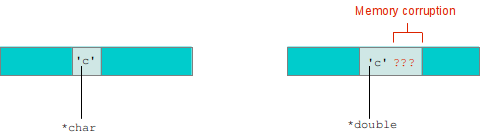
\includegraphics{images/memo_corrupt.png}
\label{memo_corrupt}
\caption{The effect on the memory of the statement: \icansi{(double*) "c"}. Firstly, a pointer to a  character is created. Secondly, the data represented by this pointer is converted into a double precision number. As the binary representation of double precision numbers is bigger than the binary representation of characters, undefined data can be accessed and memory may be corrupted.}
\end{figure}

\paragraph{High level languages} Later on, relevant bug report and safety became a prior concern. Java, which appeared in 1995, is a widely used language that attempts to provide such characteristics. In those languages, only few very little used features are able to produce unsound executable code. But, sophisticated guarding systems are needed to ensure this safety which may significantly slow down the execution. The applications written in those languages may still crash but in a more controlled and elegant way by throwing errors with relevant bug report. In Java for instance, castings are still possible, but they throw an exception when an invalid conversion occurs as in the program below:
\begin{java}
Truck t = (Truck) new Object();
t.drive();                      // undefined behavior
\end{java}
\begin{shell}
java.lang.ClassCastException: java.lang.Object cannot be cast to Truck
\end{shell}

\paragraph{Typing} Typing is the discipline that studies those "sophisticated guarding systems" introduced in the previous paragraph. Typing techniques are characterized by:
\begin{enumerate}
\item \emph{Expressiveness}: the amount of accepted sound executions.
\item \emph{Safety}: the amount of rejected unsound executions.
\item \emph{Error detection}: how early errors are detected and how relevant bug reports are.
\item \emph{Performance}: the performance costs introduced by the guards.
\end{enumerate}
We will see then that the perfect solution does not exist, compromises have to be done between those four criteria. Iterative typing is one of those compromises.

\section{Expressiveness \& Safety}

\paragraph{Language} A language is nothing more than a set, ordinary infinite, of symbol sequences called words or programs. A set of rule, called the syntax, is usually used to define the language boundary. To have any use, a language needs a semantic that associates meaning to its words. One can define multiple semantics for the same language ; for instance,\ijava{"3" + 1} has many reasonable meanings: the evaluation could return \ijava{4}, return \ijava{"31"} or simply fail.

\paragraph{Semantic} One way to define the semantic of a program is to evaluate it inside any given context, in other words to explicit the relation between its input and its output. For instance we can define the semantic of the sentence "It is sunny today." by evaluating its truth value for any kind of weather. Formally, we define the semantic of a language as a function that takes a program and some inputs then returns a value as the result of the evaluation \reffig{sem_inter}. A combination of a program and inputs is called configuration. One particular value is the error tag that indicates the semantic has failed. Notice that we can model side effects considering that the original memory is included in the input and that the transformed memory is included in the output\footnote{In this section we cautiously avoid the halting problem, we suppose that all programs terminate. We could for instance suppose that after $10^{10}$ operations, the error tag is automatically thrown.}.

\begin{figure}
\centering
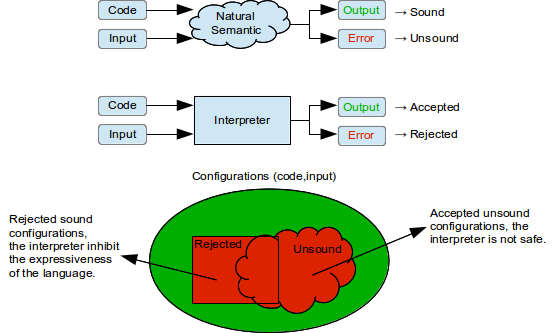
\includegraphics{images/sem_inter.png}
\caption{Given a programming language, we use two semantics: the one defined by the interpreter that is actually used and the natural one that represents an ideal.}
\label{sem_inter}
\end{figure}

\paragraph{Natural semantic} It is a semantic that the language structure naturally suggests. For instance the natural semantic used in this thesis is the standard Scheme interpreter. The natural semantic allows us to define two configuration subsets and two program subsets \reffig{sem_inter}:
\begin{itemize}
\item \emph{Sound configuration}: causes the natural semantic to succeed (not return the error tag).
\item \emph{Unsound configuration}: causes the natural semantic to return the error tag.
\item \emph{Sound input relatively to a program}: causes the natural semantic to succeed (not return the error tag) for a given program.
\item \emph{Unsound input relatively to a program}: causes the natural semantic to return the error tag for a given program.
\item \emph{Sound program}: generates some sound configurations.
\item \emph{Unsound program}: generates only unsound configurations.
\end{itemize}

\paragraph{Interpreter} The interpreter defines the semantic actually used. For practical reasons, interpreters and natural semantics may vary. In this section we focus on failure discordances not differences between successful executions. In other words, we assert that when both semantics succeed, the result is the same. In the next paragraphs, we give examples about how interpreters and natural semantics can be different. Again, we use this semantic to define two configuration subsets \reffig{sem_inter}:
\begin{itemize}
\item \emph{Accepted configuration}: causes the interpreter to succeed (not throw the error tag).
\item \emph{Rejected configuration}: causes the interpreter to throw the error tag.
\end{itemize}

\paragraph{Expressiveness} This paragraph deals with rejected sound programs which restrict the expressive power of the language. Here are some common Java restrictions:
\begin{enumerate}
\item \emph{Variables have a fixed type.} The type of a variable is fixed at the declaration, it is not possible to change it after. Next we propose a Java program with a sound semantic, it creates a new banana and eats it, but it is rejected by standard Java interpreters:
\begin{java}
Car a = new Car(); // a points to a new car
a = new Banana();  // a points to a new banana
a.eat();           // lets eat that banana
\end{java}
\item \emph{Some of the context is ignored.} Generally the execution flow is not used to track errors on Java statements. The following program is globally sound even if separately some statements cause problems:
\begin{java}
Object o = getSomething();
if(o.getClass() == Banana.class) {
	o.eat();                       // statement reached only when sound
}
if (false) {
	(new Banana()).drive();        // unreachable unsound statement
}
\end{java}
\end{enumerate}

\paragraph{Safety} This paragraph deals with accepted unsound programs. Low level languages like C allow developers to execute many unsound programs. When an unsound program is executed, either the OS layer detects an illegal operation and crashes the application, or no error is detected and the result is undefined. To bypass those restrictions introduced in the previous paragraph, high new level languages like Java also provide unsafe features that are loopholes for their safety. Here are two common unsafe features of C:
\begin{enumerate}
\item Unsafe casts:
\begin{cansi}
int a = 1;
int* b = &a;             // get the address where 1 has been stored
double* c = (double*) b; // interpreter believe b points to a double
printf("%f",*c);         // try to print the double value stored in c
\end{cansi}
\item Direct memory management:
\begin{cansi}
int* i = 123456; // erroneously consider i is an address to an integer
printf("%i",*i); // try to print the integer value stored in i
\end{cansi}
\end{enumerate}

\section{Error detection \& Performance}

\paragraph{Development cycle} For a programmer, it is very important that errors are detected early in the development cycle. Indeed the cost to correct a bug right after code writing is negligible, when bugs in a deployed application may have catastrophic consequences. Nowadays, some IDEs like Eclipse constantly analyze the code and a lot of errors are detected as soon as they are written. Further we will see that it is not possible to catch all errors as early and that testing remains an indispensable step for software development.

\paragraph{Abstraction level} Early error detection has an other advantage: it eases the debugging task. When an error is detected early, the error source is not difficult to spot and the fix is easier. Moreover, being close to the error source grants access to informations on the right abstraction level and improves the quality of bug reports.

\begin{figure}
\centering
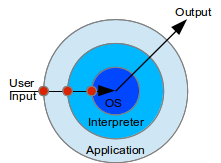
\includegraphics{images/layer.png}
\caption{User inputs may be redundantly tested at each layer.}
\label{layer}
\end{figure}

\paragraph{The agenda sample} To expose different kinds of error detections, we present a sample program that asks the user to access a random agenda:
\begin{java}
import sun.misc.Unsafe;
import java.lang.reflect.Field;

public class Agenda {
	
	static public void main(String[] args) {
		Unsafe unsafe = getUnsafe();
		long[] year = createYear(unsafe);
		System.out.println("Please input a day and a month to consult the agenda...");
		java.util.Scanner scan = new java.util.Scanner(System.in);
		int day = scan.nextInt();
		int month = scan.nextInt();
		// Month guard
		if (month < 1 || month > 12) {
			System.out.println("Month must be between 1 (January) and 12 (December).");
		} else {
			System.out.print("On the " + day + "/" + month + " we have: ");
			System.out.println(unsafe.getByte(year[(month - 1)] + (day - 1)));
		}
	}
	
	// Fill randomly a byte matrix.
	// More precisely, year is a Java array of memory address.
	// Each element of year points to a 31 byte wide memory block.
	static public long[] createYear(Unsafe unsafe) {
		java.util.Random r = new java.util.Random();
		long[] year = new long[12];
		for(int month = 0; month < 12; month++) {
			year[month] = unsafe.allocateMemory(31);
			for (int day = 0; day < 31; day++) {
				unsafe.putByte(year[month] + day, (byte)(r.nextInt() % 125));
			}
		}
		return year;
	}
	
	// Returns an Unsafe instance for direct memory management
	static public Unsafe getUnsafe() {
		Unsafe unsafe = null;
		try {
			Field field = Unsafe.class.getDeclaredField("theUnsafe");
			field.setAccessible(true);
			unsafe = (Unsafe) field.get(null);
		} catch (Exception e) {
			throw new RuntimeException("Unsafe use failed");
		}
		return unsafe;
	}
	
}
\end{java}
\begin{shell}
Please input a day and a month to consult the agenda...
19
8
On the 19/8 we have: -45
\end{shell}
At the execution we can separate those kinds of error detections:
\begin{enumerate}
\item Application detection: the application detected that the user entered a wrong input
\begin{shell}
Please input a day and a month to consult the agenda...
16
13
Wrong user input: month must be between 1 and 12
\end{shell}
\item Interpreter detection: the interpreter detected that the application asked for an illegal execution:
\begin{shell}
Please input a day and a month to consult the agenda...
5
Augustus
Exception in thread "main" java.util.InputMismatchException
	at java.util.Scanner.throwFor(Scanner.java:857)
	at java.util.Scanner.next(Scanner.java:1478)
	at java.util.Scanner.nextInt(Scanner.java:2108)
	at java.util.Scanner.nextInt(Scanner.java:2067)
	at Agenda.main(Agenda.java:12)
\end{shell}
\item OS detection: the machine detected that the Java interpreter attempted to perform an illegal operation:
\begin{shell}
Please input a day and a month to consult the agenda...
1000000000
5
On the 1000000000/5 we have: #
# A fatal error has been detected by the Java Runtime Environment:
#
#  SIGSEGV (0xb) at pc=0xb6f8b6e6, pid=8515, tid=3061922624
#
# JRE version: 6.0_24-b24
# Java VM: OpenJDK Server VM (20.0-b12 mixed mode linux-x86 )
# Derivative: IcedTea6 1.11.3
# Distribution: Ubuntu 12.04 LTS, package 6b24-1.11.3-1ubuntu0.12.04.1
# Problematic frame:
# V  [libjvm.so+0x6486e6]  Unsafe_GetNativeByte+0x66

\end{shell}
\item No detection: the application does not crash but an undefined result is perceived:
\begin{shell}
Please input a day and a month to consult the agenda...
33
5
On the 33/5 we have: 0
\end{shell}
\end{enumerate}
Those executions show how bug reports decline as errors are detected on low abstraction levels. As the abstraction level decreases, the reports have little meaning for the user and even for the programmer. Notice that in Java, as almost all the errors are caught in the two most external layers, we have to exploit very specific unsafe features to make the OS layer detect an error.

\paragraph{The client/server problem} The problematic introduced in this section is well known to software engineers and can be formulated this way: "Should I consider the client knows what he is doing?". Often the answer is NO and the developer must test all the client inputs so it can prevent him to blow up the whole server. But when layered architectures are used, the pairs client/server are multiplied and those tests become redundant \reffig{layer}.

\paragraph{Performance cost} As we saw, early error detection requires many redundant guards that can slow down the execution. If we analyze the programming language history from Assembly to Java, we see that constant efforts have been made to ease the programming task by providing abstraction and safety. At the beginning of the informatics era, performance was crucial and assembly languages proposed very low abstraction and few guards. Then human time became much more expensive than machine time and new languages privileged programming ease over performance.

\section{Introduction to type theory}

\paragraph{Typing} Typing is a strategy to detect a large class of unsound configurations for safety purposes. The concerned configurations are formally defined by the provided guards but generally typing ensures that no operations are performed out of their definition domain. People agree to say typing ensures that executions have a meaning.

\paragraph{Type} Typing techniques use types which enumerate a set of values along with operations that can be performed on them. For instance usual Java interpreters reject: \ijava{1 + "foo";} because \ijava{+} expects two arguments of type number and \ijava{"foo"} is of type string. The used type set is very dependent of the typing technique.

\paragraph{Dynamic typing} Dynamic typing is a very direct typing technique. Each computed value contains a type tag, dynamic typing raises a type error when a primitive is called with arguments containing wrong type tags. Dynamic languages are examples where the semantic defined by the interpreter is very close to the natural one. In other words, dynamic typings usually does not inhibit the language expressiveness. Drawbacks of dynamic typing include late error detection and low performance.

\paragraph{Static typing} Static typing does not have to execute programs to detect errors ; based on a static code analysis, static typings are able to detect many errors. By detecting a lot of errors statically, many guards can be removed at the execution without damaging safety. The static type checker divides the language between the accepted programs and rejected programs \reffig{express_safety}. Statically typed languages are usually characterized by early error detection, high performance but restricted expressiveness.

\paragraph{Type system} The type system is the core of the static type checker ; it formally describes the subset of the accepted programs. To be useful in practice, a type system must be decidable ; that means we must be able to separate the accepted program from the rejected one. It is easy to define undecidable type systems, for instance the type system that accepts exactly the sound programs is not decidable for any useful language in practice.

\paragraph{Static safety} Static safety is related to the amount of unsound programs rejected during static code analysis. Static safety and safety are two different concepts, dynamic languages are statically unsafe because no program is statically rejected and yet they may be safe by catching all the errors at execution time. As type systems that exactly accept sound programs are not decidable, practical type systems either accept unsound programs or reject sound programs. The first option decreases the static safety and the second decreases the expressiveness \reffig{express_safety}. 

\begin{figure}
\centering
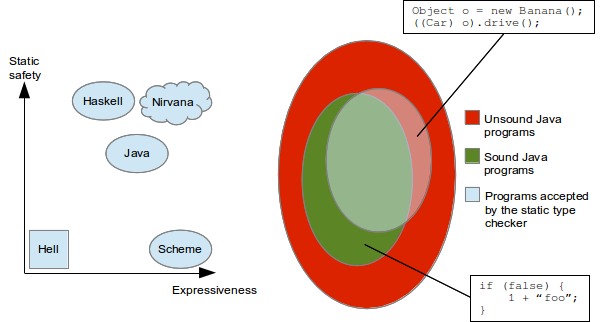
\includegraphics{images/express_safety.png}
\caption{A compromise between expressiveness and static safety must be done. Scheme is a dynamic language, therefore it does not reject statically any program and is very expressive. On the opposite, Haskell is known to be very safe. Java is an interesting example of safe language with loopholes that increase expressiveness at the cost of some safety. Finally, the "Nirvana" would be to accept exactly the sound program which is not decidable for Turing-complete languages.}
\label{express_safety}
\end{figure}

\paragraph{Loopholes} In most widely used type systems, some rules are dedicated to by-pass the other rules. In that case, we say that the type system has loopholes. Those holes aim to place the programmer over the static type checker and grant him the last word. Loopholes decrease static safety and increase expressiveness. Loopholes in high level languages like Java usually produce guards at runtime to ensure safety but other ones like C let the programmer execute unsound programs. Loopholes may be very powerful ; for instance, they can be used to express heterogeneous arrays in Java:
\begin{java}
// Accepted unsound program
Object[] array = new Object[3];
array[0] = new Car();
array[1] = new Banana();
array[2] = new Car();
Car car = (Car) array[1];       //  Casting <=> Loophole
car.drive();                    // Unsound statement
\end{java}

\paragraph{Type annotations} Static typing may need informations from the programmer to avoid ambiguous cases. The programmer may or must provide type indications for variables, parameters and expressions. In Java for instance, the annotations concern variables, parameters and return type:
\begin{java}
public float circumference(Circle c) { // Annotated parameter and return
	float pi = 3.1416;                 // Annotated variable
	return 2 * pi * c.radius();        // Static type checker verify
}                                      // this is indeed a float
\end{java}

\paragraph{Type inference} During static type checking, expressions are associated to types ; this task is called type inference. Early on, the amount of type annotations was so important that this task was trivial. But nowadays, languages tend to let programmers decide where they want to put type annotations ; this freedom complicates the inference task and sometimes type annotations are still required to avoid ambiguities. For instance in C\#, the keyword \icsharp{var} allows to automatically deduce the type of the initializer expression: \icsharp{var x = "Yo";} is equivalent to \icsharp{String x = "Yo";}.

\paragraph{Scripted languages \& compiled languages} Often, dynamically typed languages are directly executed, then they are called scripting languages. On the other hand, as statically typed programs must be analyzed anyway, they are often compiled before being executed. For instance Java programs are compiled into portable byte codes before execution.

\paragraph{Recapitulation} In this section we saw how dynamic and static typing usually catch errors. We also introduced the important concept of static safety which is orthogonal to the expressiveness ; no typing can be entirely statically safe without inhibiting the language expressiveness. Finally some classic concepts in type theory: loopholes, type annotation and type inference.

\section{Comparison between static and dynamic typing}

There is a religious war since decades between the static typing defenders and the supporters of dynamic typing. The first ones appreciate the reliability and the organization of the static programs when the second ones highlight the expressiveness and the flexibility of dynamic languages. Static and dynamic typing have always cohabited \reffig{histo} but before the explosion of Internet applications, only statically typed languages where widely used in practice. Indeed we will see that dynamic typing fits well the needs of web developers. The rest of this section is a succession of comparisons between static and dynamic typing.

\begin{figure}
\centering
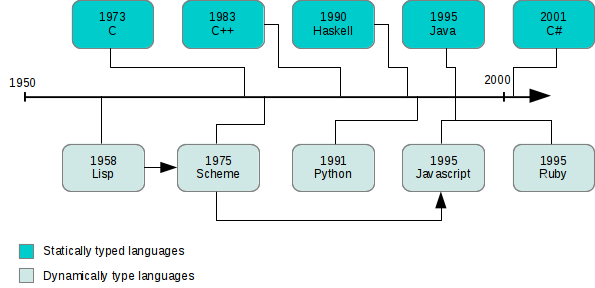
\includegraphics{images/histo.png}
\caption{Apparition of some programming languages. JavaScript is an adaptation of Scheme which is itself an evolution of Lisp.}
\label{histo}
\end{figure}

\paragraph{Safety} In a static typing, type errors are detected very early in the development process (some development platforms like Eclipse detect type errors as soon as the programmers writes it). When in dynamic typing, type errors are detected at the last possible moment ; type errors may occur during the use of a finished product. That is why statically typed languages are reputed more reliable. As a response, dynamic typing supporters may argue that testing can catch much more errors. But testing is a very expensive verification process that never reaches 100\% coverage.  

\paragraph{Blame} In dynamic languages, type errors may be detected very deep inside a library because a call was made with the wrong types. As a result, the programmer gets a very irrelevant bug report like "true is not a number" spotted in some dark place he never saw. Generally, dynamic typing fails to blame the correct piece of code when a type error occurs. A lot of efforts are being made to get more relevant bug reports on those languages \refch{ch_related}.

\paragraph{Expressiveness} As said before, in a Turing-complete language it is impossible to separate the safe programs from the unsafe ones. In practice, no type system accepts all safe programs (the provided guaranties would be too weak) ; so they all have their limitations. Type systems tend to be improved to be able to express more and more concepts. Those refinements are a very difficult task and may easily lead to type systems without enough guards or unusable in practice. An example of such refinement is the genericity introduced in Java in 2004. Indeed before, the Java type system could not express the identity function that just returns its argument and casts had to be used:
\begin{java}
public static Object identity(Object o) {
	return o;
}

public static void main(String[] args) {
	Banana b = (Banana) identity(new Banana()); // pollution cast, never fails
	b.eat();
	Car c = (Car) identity(new Car());          // pollution cast, never fails
	c.drive();
}
\end{java}
As this kind of program has practical interests, the Java type system has been improved with genericity:
\begin{java}
public static T <T> identity(T t) {
   return t;
}

public static void main(String[] args) {
	identity(new Banana()).eat(); // no pollution cast
	identity(new Car()).drive();  // no pollution cast
}
\end{java}

\paragraph{Maintenance} The last point can be analyzed from an other point of view: as static type checker forces the programs to be consistent and very organized they are easier to maintain. On the other hand, dynamic typing is so permissive that programs may quickly become inconsistent as the project grows. When a modification has to be done on a static programs, the static type checkers detect most of the spots where the code has to be updated. 

\paragraph{Flexibility} Again the last point may be turned around and because of type annotations, the purpose of most of those updates is to satisfy the type system without changing the semantics. So type annotation can be a burden when quick fixes must be done. In response of this argument, most statically typed languages develop type inference to let the programmer decide where he put type annotation.

\paragraph{Performance} Because of the assumptions made on the accepted static programs, the static interpreters have to perform less type checks than the interpreters of dynamic languages. Moreover values of a statically typed language can be stored in a more efficient representation (the original motivation to introduce type in C).

\paragraph{Documentation} A lot of things can be deduced from the type signature of a procedure ; while dynamic programs can only provide meaningful names as built-in documentation. This drawback can be countered by very complete documentations like in Perl.

\paragraph{Recapitulation} In \reftab{pc_stat_dyn} we summarize the main advantages and drawbacks of static typing (annotated or not) and dynamic typing. It comes out that static typing is good for large projects with a long life cycle when dynamic typing is good for prototyping. Static typing is used a lot on critical domain when dynamic typing is very used on domains where development speed is a prior concern like Internet applications development. As it appears that neither static typing nor dynamic typing are perfect a lot of investigations are currently performed to mix the best of those two worlds.

\begin{table}
\centering
\begin{tabular}{|p{3.5cm}|p{3.5cm}|p{3.5cm}|p{3.5cm}|}
\hline
& \multicolumn{2}{|c|}{Static typing} & \multicolumn{1}{|c|}{Dynamic typing}\\
& \multicolumn{1}{|c|}{Not much inference} & \multicolumn{1}{|c|}{Hard inference} &\\ 
\hline
\hline
Safety & \multicolumn{2}{|p{7cm}|}{\pro Very early in the development process.}&\cons At the last possible moment.\\
\hline
Blame &\multicolumn{2}{|p{7cm}|}{\pro Relevant bug report.} &\cons Irrelevant bug report spotted on bad places.\\
\hline
Expressiveness &\multicolumn{2}{|p{7cm}|}{\cons Limited by the type system.}&\pro No limitation compared to runtime semantic.\\
\hline
Maintenance (large project) &\multicolumn{2}{|p{7cm}|}{\pro Forces structured and consistent programs.}&\cons Modifications may lead to unsuspected errors.\\
\hline
Flexibility (small \& medium project) & \cons Code updates are very concerned by type system restrictions. & \even Some updates are concerned by types system restrictions. & \pro Code updates only concern the semantic. \\
\hline
Performance &\multicolumn{2}{|p{7cm}|}{\pro Less type check, efficient representation.}&\cons Type checks at each primitive application, representations must carry types.\\
\hline
Documentation &\pro Type signature is a good way to describe a procedure. &\even Programmer dependent. &\cons Only rely on the procedure name.\\
\hline
\end{tabular}
\caption{Pro and cons of dynamic typing and static typing (with a variable type inference presence). Dynamic typing is better for prototyping and static typing is better for large projects with a long life cycle.}
\label{pc_stat_dyn}
\end{table}

\section{Iterative typing as a compromise}

Mixing static and dynamic typing is currently a field heavily investigated. It is about performing as much static type checks as possible and leaving as little runtime checks as possible to ensure safety. By following this direction, we expose here what problem iterative typing attempt to solve. From now on, we suppose the reader is familiar with Scheme ; if not a gentle introduction can be found at \refan{an_scheme}

\paragraph{Dynamic reading} A much used primitive in Scheme is \ischeme{read}, in this thesis we assume \ischeme{read} may either return a boolean, a number or a string\footnote{The read procedure actually return a s-expression but simple constants suffice to expose the problem we attempt to resolve.}. A common problem Scheme programmers encounter is late type error detections in case the return type of \ischeme{read} has not been manually checked:
\begin{scheme}
(define x (read))

;; Many lines later...

(* 2 pi x)
\end{scheme}
In the above code, if the \ischeme{read} call did not return a number, the program raises an error at the last statement. We want to detect this error earlier, ideally right at \ischeme{read} call, without reducing the expressiveness too much.

\paragraph{Dynamic conditional structure} When a conditional structure modifies the type deduction depending on the branch actually executed, we say it is dynamic. Such dynamic behavior may have two aspects:
\begin{enumerate}
\item \emph{Uncertain return}: depending on the executed branch, the evaluation of a \ischeme{if} expression may return values of different types. The below Scheme program returns either an error message or the division result: 
\begin{scheme}
(define (divide x y)
  (if (= y 0)
      "division by zero" ;; a string is returned
      (/ x y)))          ;; a number is returned
\end{scheme}
The first branch returns a string and the second returns a number.
\item \emph{Uncertain use}: depending on the executed branch, the use of variable is modified. The Scheme program below returns a convenient description of a \ischeme{divide} result:
\begin{scheme}
(define (main x)
  (if (string? x)
      (concat "Error: " x)                     ;; x is used as a string
      (concat "Result: " (number->string x)))) ;; x is used as a number
\end{scheme}
The first branch uses the given argument, \ischeme{x} as a string and the second branch uses \ischeme{x} as a number.
\end{enumerate}
What static type systems do concerning conditional structure is assume both branches will be executed and so impose that they are type compatible. As a result static type system systematically reject dynamic conditional structure. We want to support such conditional structures and still be able to detect errors early.

\paragraph{Improve expressiveness} The biggest drawback of static type systems is the expressiveness inhibition. A lot of investigations have been done to increase the expressiveness of statically typed language. Those efforts can be split into two directions:
\begin{enumerate}
\item \emph{Pure static typing}: Complicate type systems to grab as many safe programs as possible. The Haskell type system is a successful result of this direction: it is believed safe and yet very expressive. 
\item \emph{Loopholes}: Intentionally introduce loopholes in the type system. Those loopholes decrease the static safety and require additional guards at runtime to ensure safety. Loopholes are the usual way to mix static and dynamic typing. This direction is currently under high investigation which has led to the creation of new typings like soft and gradual typings \refch{ch_related}.
\end{enumerate}

\paragraph{Iterative typing} The solution presented in this thesis, called iterative typing, follows the loophole direction. Iterative typing recognizes there are dynamic events, like \ischeme{read} calls and dynamic conditional structures, that require runtime information to be analyzed precisely. Those events are accepted thanks to loopholes inside the type system and will generate annotations so that type checking can be fulfilled at runtime when more information are available.

\section{Conclusion}

In this chapter we exposed some of the most important concept of type theory. In particular we saw that it is not possible to design a type system that accepts exactly the sounds programs ; in practice, type systems must do a compromise between static safety and expressiveness. We then highlight the gap between static and dynamic typing and argued that errors in some very dynamic patterns could be detected much earlier than dynamic typed languages usually do.

%%%%%%%%%%%%%%%%%%%%%%%%%%%%%%%%%%%%%%%%
%%%%%%%%%%%%%%%%%%%%%%%%%%%%%%%%%%%%%%%%
%%%%%%%%%%%%%%%%%%%%%%%%%%%%%%%%%%%%%%%%
%%%%%%%%%%%%%%%%%%%%%%%%%%%%%%%%%%%%%%%%
\chapter{Approach \& Implementation\label{ch_approach}}
%%%%%%%%%%%%%%%%%%%%%%%%%%%%%%%%%%%%%%%%
%%%%%%%%%%%%%%%%%%%%%%%%%%%%%%%%%%%%%%%%
%%%%%%%%%%%%%%%%%%%%%%%%%%%%%%%%%%%%%%%%
%%%%%%%%%%%%%%%%%%%%%%%%%%%%%%%%%%%%%%%%

This chapter is a gentle introduction to iterative typing. After this chapter, the reader should know what iterative typing is capable of and have some intuition about how iterative typing is implemented. In the first section we define an ideal iterative typing for Scheme without polymorphism or recursion. On the next section we expose the whole iterative framework as an approximation of the iterative ideal. The third section exposes how the core of iterative typing has been extended to support polymorphism. The next section is a discussion about the implementation of recursions in iterative typing. The chapter ends with the presentation of some features specific to iterative typing.

\section{Iterative typing's ambition}

In this section we reason about a non recursive subset of Scheme. This assumption will allow us to define an ideal algorithm for the iterative typing. This algorithm would never reject a rightful execution and would catch all the unsound combinations of program and input as soon as possible. This ideal motivates the whole iterative type system, it is the core idea of this thesis.

\paragraph{Inputs as a trace} A trace is a sequence that represents all the inputs a program will receive. Without recursion, a Scheme program reads its input incrementally and we can assume the amount of required inputs is finite. As an example we present a simple program, its execution and the associate trace:
\begin{scheme}
(display "What is your name?\n")
(define name (read))
(display "What is your age?\n")
(define age (read))
(display "Where do you live?\n")
(define place (read))
(define majority 18)
(if (< age majority)
    (display "You are too young...\n")
    (display (concat "Hello " name " of " place "!\n"))
;; Normally concat have an arity of 2 but for clarity reasons we use multiple arguments.
\end{scheme}
\begin{shell}
What is your name?
"Laurent"
What is your age?
22
Where do you live?
"Brussels"
Hello Laurent of Brussels!
\end{shell}
The program asks the user some information and then displays a personalized message. In the above execution, the input trace is: \ischeme{("Laurent" 22 "Brussels")} ; \ischeme{"Laurent"} has been stored into the variable \ischeme{name}, \ischeme{22} into \ischeme{age} and \ischeme{"Brussels"} into \ischeme{place}. This example will be used throughout the rest of this section and will be referred as the "name-age-place" program.

\paragraph{Sound/Unsound traces} An input trace is sound relatively to a program when the natural semantic does not return an error if the program is executed with that trace. Here, the natural semantic is given by a standard Scheme interpreter. On the other hand, unsound traces combined with the associated program cause the Scheme interpreter to raise an error. Below we present an unsound and a sound trace relatively to the name-age-place program with their associated execution:
\begin{enumerate}
\item The trace \ischeme{(1234 22 "Brussels")} is unsound because \ischeme{name} is used as a string in that execution:
\begin{shell}
What is your name?
1234
What is your age?
22
Where do you live?
"Brussels"
ERROR: concat: expects type <string> as 2nd argument,
       given: 1234; other arguments were: "Hello "
\end{shell}
\item The trace \ischeme{(1234 17 "Brussels")} is sound because the taken path (the else branch) does not force the name to be a string:
\begin{shell}
What is your name?
1234
What is your age?
17
Where do you live?
"Brussels"
You are too young...
\end{shell}
\end{enumerate}

\paragraph{The iterative ideal} As the execution goes on, the head of the input trace is specified which restricts the number of traces that remain possible \reffig{trace}. If all the remaining traces are unsound, the ideal iterative would throw an error. So by definition, the iterative ideal throws an error as soon as possible, way before illegal operations are actually performed. This is the aim of iterative typing and the core idea of this thesis. The iterative ideal maximizes three of the four main criteria concerning type systems, the only drawback being the performance cost \reftab{ideal_iter_crit}. Indeed the amount of traces to analyze makes the iterative ideal unusable in practice. Lets illustrate this ideal with two examples concerning the "name-age-place" program:
\begin{itemize}
\item There is no sound trace that starts by \ischeme{(1234 22)}. So if \ischeme{1234} is entered for the name and \ischeme{22} for the age, the ideal iterative would immediately throw an error with the following message: "If the first input is not a string then the second input must be a number smaller than 18".
\item Again, the specification \ischeme{("Laurent" "boum")} discriminates any sound trace. The iterative ideal would throw an error with the message: "The second input must be a number."
\end{itemize}

\begin{table}
\centering
\begin{tabular}{|p{5cm}|p{5cm}|}
\hline
Criterion & Iterative ideal\\
\hline
\hline
Safety & All the errors are detected.\\
\hline
Expressiveness & No sound execution is rejected.\\
\hline
Error detection & As soon as possible with relevant bug report.\\
\hline
Peformance & The computation is probably very high due to the amount of trace to analyze.\\
\hline
\end{tabular}
\caption{The iterative ideal maximize three out of four criteria concerning type systems.}
\label{ideal_iter_crit}
\end{table}

\begin{figure}
\centering
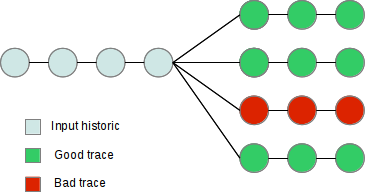
\includegraphics{images/trace.png}
\caption{The available trace during an execution. As soon as no sound trace remains, the ideal iterative typing would throw an error.}
\label{trace}
\end{figure}

\paragraph{Computability of the ideal} We give two direction to implement the iterative ideal:
\begin{itemize}
\item \emph{Exhaustive testing}: The iterative ideal can be achieved by executing the program on each different trace. Obviously, the set of trace to analyze is way to large and this solution is not feasible. 
\item \emph{Constraints on trace}: By performing a static code analysis we can deduce constraints that defines the set of sound traces. For the name-age-place program those constraints for any trace $(name,age,place)$ would be:
$$\left\{\begin{array}{l}
typeOf(age)=Number\\
age > 18 \Rightarrow (typeOf(name) = typeOf(place) = String)\\
\end{array}\right.$$
Demonstrations that mix values and types to prove the safety of programs is the domain of dependent typing. Dependent typing is a very powerful tool but requires the programmer's help to provide those safety proofs which does not fit our problem statement\cite{dep}.
\end{itemize}
So the first option is not feasible and the second is too complicated to use. At that point we, naturally conclude that some errors cannot be detected by iterative typing and reduce the working precision from values to types.

\paragraph{The type approximation} In the type approximation, we work only with types instead of precise values. In consequence, the input traces become lists of types instead of lists of values. The drawback is that we do not have access to all values anymore. This is a problem when types depend on values ; the \icode{if} statement can induce such dependency: for instance, the type of \ischeme{(if x 1 "foo")} can, depending on the value of \ischeme{x}, be either a number or a string. In consequence, we are forced to consider conditional structures as dynamic events just like inputs. For the "name-age-place" program, the trace $(String,Number,String,else)$ is sound and means that: a string was first entered, the second input was a number, the last input was a string and the else branch of the conditional structure was evaluated. We give some other examples in \reftab{approx_trace}.

\begin{table}
\centering
\begin{tabular}{|l|p{5cm}|}
\hline
Trace & Soundness \\
\hline
$(String,Boolean,String,then)$ & Unsound trace: the second input must be a number.\\
\hline
$(String,Number,String,then)$ & Sound trace.\\
\hline
$(Number,Number,String,else)$ & Unsound trace: if the first input is not a string, the "then" branch must be executed.\\
\hline
$(Number,Number,String,then)$ & Sound trace.\\
\hline
\end{tabular}
\caption{Soundness of several traces for the "name-age-place" program.}
\label{approx_trace}
\end{table}

\paragraph{Value errors} The division by zero error is an example of value errors. The division operator is only defined for a subset of the number set, we say that zero is a gap in its definition. Generally value errors arise when an operator has an undefined behavior even when the given arguments have the rightful types. An other common example of value error is the null pointer exception: the Scheme statement \ischeme{(car null)} is type safe but unsound because the \ischeme{car} operation is not defined for the null list. By working with type instead of values we can not detect value errors anymore.

\paragraph{Iterative typing} Even if the type approximation considerably reduces the amount of traces to analyze, their number still exponentially grows with the amount of inputs and conditional structures. Exponential computation time algorithm are not practically acceptable and so iterative typing uses a system of constraint on traces instead of an exhaustive research. For the name-age-place programs, those constraints on the trace $(name,age,place,branch)$ would have been:
$$\left\{\begin{array}{l}
age = Number\\
(branch = else)\Rightarrow (name = place = String)\\
\end{array}\right.$$

\paragraph{Conclusion} Typically, when static typings encounter an uncertainty, they make assumptions to carry on the static analysis. Those assumptions inhibit the expressiveness of the language and iterative typing drops constraints inside the code instead. Those annotation will be used at the execution to fulfill the type checking when more information will be available. By doing this, iterative typing can handle very dynamic code like the name-age-place program and is still able to detect error earlier than dynamic typing on more relevant place. The advantage of iterative typing is highlighted below by two executions of the "name-age-place" program:
\begin{enumerate}
\item Iterative typing accepts more sound executions than static typing:
\begin{itemize}
\item Static execution:
\begin{shell}
Inter >> What is your name?
"Laurent"
What is your age?
17
Where do you live?
1234
TYPE ERROR: expects a string
\end{shell}
\item Iterative execution:
\begin{shell}
Inter >> What is your name?
"Laurent"
What is your age?
17
Where do you live?
1234
You are too young...
\end{shell}
\end{itemize}
\item Iterative typing detects type error sooner than dynamic typing on more relevant places:
\begin{itemize}
\item Dynamic execution:
\begin{shell}
What is your name?
"Laurent"
What is your age?
"boum"
Where do you live?
"Brussels"
TYPE ERROR: > expects two arguments of type number give a string and a number
\end{shell}
\item Iterative execution:
\begin{shell}
What is your name?
"Laurent"
What is your age?
"boum"
TYPE ERROR: expects a number
\end{shell}
\end{itemize}
\end{enumerate}

\section{The iterative framework}
  
Now we know more precisely what iterative typing attempts to achieve, we will present informally how it is implemented. Iterative typing performs a static typing that does not make any assumption when a dynamic event occurs \reffig{iter_comp_inter}. The static type checker performs as many checks as possible and puts annotations inside the code where a dynamic event occurs.

\begin{figure}
\centering
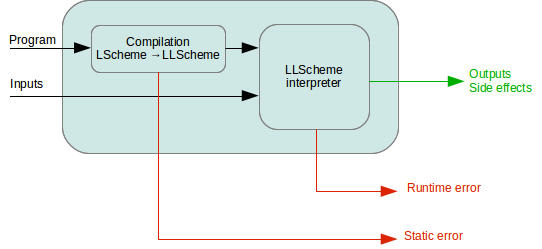
\includegraphics{images/iter_comp_inter.png}
\caption{The atomic Scheme subset is compiled before being executed.}
\label{iter_comp_inter}
\end{figure}

\paragraph{LScheme} LScheme is a Scheme-like language that we will evaluate with an iterative interpreter. Beside continuation, LScheme supports all the Scheme core features. LScheme also includes some special forms specific to iterative typing that we will see further.

\paragraph{LLScheme} LLScheme is the annotated version of LScheme that contains the constraints exposed before. Those constraints have the form \ischeme{a => t} which means the type variable \ischeme{a} is instantiated to \ischeme{t}. The two kind of dynamic events that currently require annotations are:
\begin{enumerate}
\item \emph{Input procedure}: The primitive \ischeme{read} asks the user to enter some data, the returned constant can be of type boolean, number or string. The annotated call to \ischeme{read} has the following form: \ischeme{(sub [in => t] read)} which means that the input is expected to be of type \ischeme{t}. Here is an example:
\begin{scheme}
(define x ((sub [in => a] read)))      ; the input can be any constant
(define y ((sub [in => Number] read))) ; the input must be a number
(+ y 1)
\end{scheme} 
\item \emph{Conditional structure}: Each branch of the \ischeme{if} expression contains an annotation of the form: \ischeme{[cond => t, a1 => t1, ...]} which means that the type variable \ischeme{cond} is instantiated to \ischeme{t}, \ischeme{a1} is instantiated to \ischeme{t1}, etc. Usually, the type variable \ischeme{cond} denotes the type of the whole conditional structure. The \ischeme{if} statement is dynamic in two different ways:
\begin{enumerate}
\item The \ischeme{if} statement can return two different types:
\begin{scheme}
(if x
    [cond => Number] 1      ; the if returns a number
    [cond => String] "foo") ; the if returns a String
\end{scheme}
\item Depending on the taken branch, the type deduction differs:
\begin{scheme}
(define x (({in => a} read)))                           ; x can be anything
(define y (({in => b} read)))
(if y
    [a => String, cond => String] (concat "yo" x) "ok" ; x must be a string
    [a => Number, cond => String] (+ 1 x) "ok")        ; x must be a number
\end{scheme}
\end{enumerate}
\end{enumerate}

\paragraph{Compilation LScheme $\to$ LLScheme} Though it is possible, the programmer is not supposed to write LLScheme annotations himself. Instead the iterative framework embeds a compiler that compiles LScheme to LLScheme by automatically inserting rightful annotations. This compilation is based on type inference and will be detailed in \refch{ch_theory}.

\paragraph{Locus} A locus is nothing more than the union of all the constraints generated during the execution by the previous dynamic events. Loci are used to keep track of the previous dynamic events and detect incompatibilities between constraints. The incorporation of new constraints inside the current locus is done via the unification algorithm \cite{hm2}. We will not describe this algorithm here ; instead, we give some examples at \reftab{compa_constr}.

\begin{table}
\centering
\begin{tabular}{|l|l|}
\hline
\multicolumn{1}{|c|}{Original constraints} & \multicolumn{1}{|c|}{Unified constraints}\\
\hline
\hline
\icode{a => d -> c} & \icode{a => d -> String}\\
\icode{b => [c]} & \icode{b => [String]}\\
\icode{c => String} & \icode{c => String}\\
\hline
\hline
 & \icode{a => String}\\
\icode{a -> b => String -> (c -> Boolean)} & \icode{b => Number -> Boolean}\\
\icode{[d] => c} & \icode{c => [Number]}\\
\icode{e -> c = Number -> [Number]} & \icode{d => Number}\\
 & \icode{e => Number}\\
\hline
\hline
\icode{a => b -> [Boolean]} & Failure: incompatible type\\
\icode{a -> Number => (Number -> [String]) -> Number)} & \icode{Boolean => String}\\
\hline
\hline
\icode{a => b -> Boolean} & Failure: infinite type on\\
\icode{b => [b]} & \icode{a => [a] -> Boolean}\\
\hline
\end{tabular}
\caption{On the left: the original constraints, on the right the resolved ones.}
\label{compa_constr}
\end{table}

\paragraph{Interpretation of LLScheme} The execution always starts with the empty locus which obviously contains no constraint. Then the locus is carried around and affected by dynamic events. This suggests that the locus follows exactly the execution flow and that compound procedures must manipulate the locus present during the application \reffig{mono_proc}. Below we explain how the annotations of \ischeme{read} and \ischeme{if} affect the current locus:
\begin{itemize}
\item \emph{Input procedure}: Given the annotated reading procedure: \ischeme{(sub [in => a] read)}, if the input type was \ischeme{b} the constraint \ischeme{a => b} will be incorporated to the current locus.
\item \emph{Conditional structure}: The constraints added when a \ischeme{if} statement is reached correspond to the constraints stored inside the executed branch. So when \ischeme{(if x [a => String] "foo" [a => Number] 1)} is reached, depending on the value of \ischeme{x}, either \ischeme{a => String} or \ischeme{a => Number} will be incorporated.
\end{itemize}

\begin{figure}
\centering
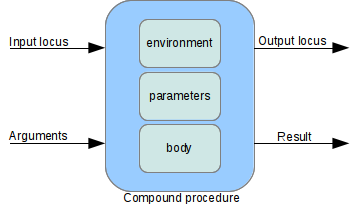
\includegraphics{images/mono_proc.png}
\caption{In iterative typing, procedures not only affect values but also the current locus. Unlike environments, loci are not encapsulated in compound procedures ; instead, it is the locus present at the application that is used.}
\label{mono_proc}
\end{figure}

\paragraph{The "name-age-place" example} It is easy to insert the correct annotations inside the "name-age-place" program. Below we expose the annotated program and on \reffig{constr_name_age_place} we graphically expose a possible execution.
\begin{scheme}
(display "What is your name?\n")
(define name ((sub [in => a] read)))            ; No constraint on the first input
(display "What is your age?\n")
(define age ((sub [in => Number] read)))        ; Second input must be a number
(display "Where do you live?\n")
(define place ((sub [in => b] read)))           ; No constraint on the third input
(define majority 18)
(if (< age majority)
    ; The first and third input must be strings
    [a => String, b => String] (display (concat "Hello " name " of " place "!\n"))
     ; No constraint on the else branch
    [] (display "You are too young...\n"))
       
\end{scheme}

\begin{figure}
\centering
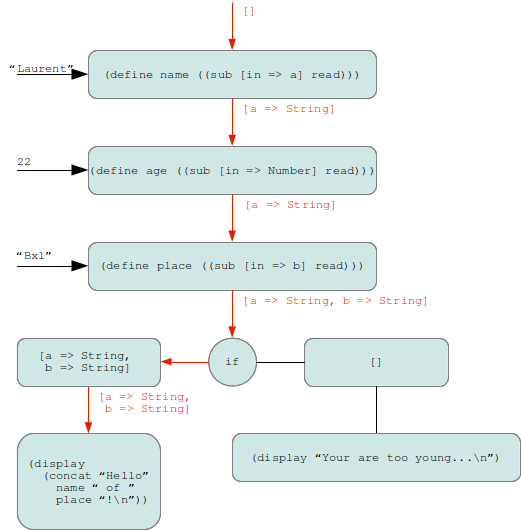
\includegraphics{images/constr_name_age_place.png}
\caption{The evolution of the locus through the execution of the "name-age-place" program with the inputs \ischeme{"Laurent"}, \ischeme{22} and \ischeme{"Bxl".}}
\label{constr_name_age_place}
\end{figure}

\section{LScheme \& polymorphism}

\paragraph{The identity procedure} A procedure is said polymorphic when it can be called with different types. For instance, in Scheme, the primitives that manipulate lists are polymorphic ; both \ischeme{(cons 1 null)} and \ischeme{(cons "foo" null)} are accepted. In dynamic typing, polymorphism support is automatically granted since the arguments of compound procedure are not type checks. On the other hand it is not trivial to support polymorphism in statically typed language. If Scheme did not support polymorphism, the following program would be rejected:
\begin{scheme}
(define identity (lambda (x) x))
(identity 1)
(identity "foo") ; Static type error: Number cannot be converted to String
\end{scheme}
When it has a sound Scheme semantic:
\begin{shell}
1
"foo"
\end{shell}

\paragraph{The map procedure} While Scheme does not enforce it, programmers typically make and use homogeneous lists. Homogeneous lists are lists where each element has the same type. The map function is an example of a procedure that manipulates such lists:
\begin{scheme}
(define map (lambda (f xs)
              (if (null? xs)
                  null
                  (cons (f (car xs)) (map f (cdr xs))))))

(define incr (lambda (x) (+ x 1)))
(define concat-hello (lambda (x) (string-append "hello " x)))

(map incr (cons 1 (cons 2 null)))                 ; map called with a list of number
(map concat-hello (cons "foo" (cons "bar" null))) ; map called with a list of string
\end{scheme}
Again, this program would fail without polymorphic support when it has a sound semantic:
\begin{shell}
(2 3)
("hello foo" "hello bar")
\end{shell}
What comes out of those examples is that Scheme without polymorphism is not Scheme anymore. Polymorphism is a feature in static typing that can not be by-passed nowadays and therefore must be supported by iterative typing.

\paragraph{The polymorphic wrapper} To simulate polymorphism the current iterative prototype uses a wrapper around monomorphic procedures \reffig{poly_proc}. Essentially, this wrapper adds constraints before the monomorphic application and then releases them to allow a further call with different types. Practically polymorphic procedures are defined on \ischeme{define} statement but the wrapper is created at each time the polymorphic procedure is referenced by an identifier.

\begin{figure}
\centering
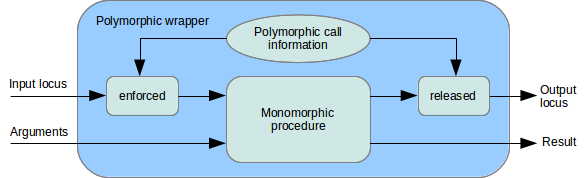
\includegraphics{images/poly_proc.png}
\caption{Polymorphism is simulated by a wrapper that modifies the locus before and after the monomorphic call.}
\label{poly_proc}
\end{figure}

\paragraph{Polymorphic calls} All the information required by the wrapper is stored where the polymorphic procedure is pointed by an identifier. Indeed, each identifier that refers to a polymorphic value is annotated in LScheme. It is important to notice that those polymorphic annotations are safe and cannot transform the current locus into an incompatible set of constraints. So basically, type errors cannot appear at polymorphic calls and therefore polymorphic calls should not be considered as dynamic events. This behavior is in accordance with the iterative philosophy where type errors are spotted only where ambiguities arise.

\paragraph{A polymorphic example} Here is an example that illustrates how the polymorphic wrapper works. 
\begin{scheme}
(define (evil x) 
  (if x
      1
      "fool"))
(+ 1 (evil #t))
(concat "yo " (evil #f))
\end{scheme}
The above program can be annotated into:
\begin{scheme}
(define (evil x) 
  (if x
      [a => Number] 1
      [a => String] "fool"))
(+ 1 ((sub [a => Number] evil) #t))
(concat "yo " ((sub [a => String] evil) #f))
\end{scheme}
So when the statement \ischeme{(+ 1 ((sub [a => Number] evil) #t))} is reached, the current locus is empty and the constraint \ischeme{a => Number} is added. Then we proceed to a monomorphic call of the compound procedure \ischeme{evil}. The \ischeme{then} branch being taken, the constraint \ischeme{a => Number} is added and the current locus is still \ischeme{a => Number}. Then when the monomorphic call returns we release the constraint \ischeme{a => Number} and we get the empty locus again. The current locus being empty, we can evaluate the second call to \ischeme{evil} without restriction.

\paragraph{Read as a polymorphic procedure} Actually \ischeme{(sub \{in => t\} read)} is not a special case but just a call to a polymorphic procedure. The \ischeme{read} polymorphic procedure can indeed be implemented with primitive procedure \ischeme{read-line} that returns the string the user just input:
\begin{scheme}
(define (read)
  (let (input (read-line))
    (cond ([in => String]  (input-string? input)  (input->string input))
          ([in => Number]  (input-number? input)  (input->number input))
          ([in => Boolean] (input-boolean? input) (input->boolean input))
          ([in => void]     else                  (error "unknown type")))))
\end{scheme}

\section{LScheme \& recursion}

\paragraph{Implementation} Scheme provides many ways to create recursive processes ; one of them is based on the \ischeme{define} special form. Indeed, in the definition \ischeme{(define <name> (lambda (<params>) <body>))}, the identifier \ischeme{<name>} can be used inside \ischeme{<body>}. This is the mean we chose to support recursion in LScheme. To achieve recursion we need the environment inside the compound procedure to contain binding of \ischeme{<name>} that points to the whole structure \reffig{mono_rec}. Such implementation is the usual way to implement recursion and is not problematic when combined with iterative typing.

\begin{figure}
\centering
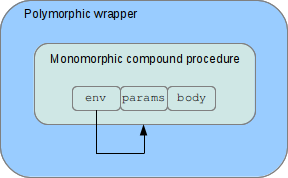
\includegraphics{images/mono_rec.png}
\caption{The environment of a recursive compound procedure contains a binding to itself.}
\label{mono_rec}
\end{figure}

\paragraph{Monomorphic recursion} So the statement \ischeme{(define <name> (lambda (<params>) <body>))} creates a compound procedure that appears monomorphically inside \ischeme{<body>} but polymorphically in the rest of the program. Such recursion is called monomorphic and the types that appear inside the body do not change during the whole recursion. The map function is an example of monomorphic recursion. Monomorphic recursion is powerful enough to fit the programmer's everyday needs and that is why recursion is almost always monomorphic in statically typed languages.

\paragraph{Monomorphic recursion \& iterative typing} However, monomorphic recursion has particular consequence in iterative typing. Because the type that does not affect the outside world is fixed as well, some unfortunate restrictions appear. Lets present a simple loop that asks for an input and then displays it:
\begin{scheme}
(define forever (lambda ()
                   (define x ((sub [in => a] read)))
                   ((sub [out => String] display) "input: ")
                   ((sub [out => a] display) x)
                   ((sub [out => String] display) "\n")
                   (forever)))
(forever)
\end{scheme}
Because the type of the input, \ischeme{a} in the above program, has no consequence at all for the rest of the recursion, we naturally expect that the type of the input can be modified from one recursive call to an other. Well, this is currently not the case in iterative typing ; all the types involved in the recursion are fixed. As a result, the first input fixes the type of all the future inputs ; as soon as the user enters a value of a different type, an error is raised:
\begin{shell}
 1
input: 1
2
input: 2
3
input: 3
"BOUM"
TYPE ERROR
\end{shell}

\section{Iterative special forms}

Until now, LScheme was nothing more than a subset of Scheme. Here we introduce three special forms that are specific to iterative typing. The first two special forms \ischeme{if-static} and \ischeme{unsafe} do not actually increase the Scheme semantic and just concern error detections. However, the last special form, \ischeme{if-viable} is not expressible in Scheme and must be used very carefully.

\paragraph{Static conditional structure} Iterative typing grants the programmer the power to choose whether a conditional structure should be statically checked or dynamically checked, as it was always the case so far. Static conditional structures, denoted by the special form \ischeme{(if-static <pred> <then> <else>)}, are analyzed in the same way as pure static typings usually do. In particular, the branches must be type-compatible and no annotations are inserted during the compilation from LScheme to LLScheme. Programs that contain no dynamic conditional structure are statically type safe and although annotations on polymorphic calls still remain, the constraint system never raises an error. For instance, if we implement the classic conditional structure that returns two different types following the executed branch with \ischeme{if-static}, then an error will be raised at compile time:
\begin{scheme}
(define (evil x)
  (if-static x 1 "foo"))
\end{scheme}
\begin{shell}
Type error: Number is not compatible with String.
\end{shell}

\paragraph{Unsafe execution} By using the special form \ischeme{(unsafe <body>)}, the programmer is able to perform an unsafe executions of the statements contained in \ischeme{<body>}. More specifically, if a constraint incompatibility is detected inside \ischeme{<body>} the iterative constraint systems is shutdown and the execution becomes unsafe.
\begin{scheme}
(unsafe
 (define x ((sub [in => Number] read)))
 ((sub [out => String] display) "Still running...")
 (+ 1 x))
\end{scheme}
\begin{shell}
>> "bar"
Still running...
+: expects type <number> as 2nd argument, given: "bar"; other arguments were: 1
\end{shell}
Without the wrapping inside \ischeme{unsafe}, the above program would predict the error right inside the \ischeme{read} procedure. The unsafe special form allows to execute the program until errors actually happen.

\paragraph{Viability test} The special form \ischeme{(if-viable <attempt> <else>)} allow to test if the executing \ischeme{<attempt>} with the current dynamic information is safe. In other words, \ischeme{<attempt>} is executed only if iterative typing does not predict an error for that execution. As this special form can not be expressed in Scheme it must be used with caution. Below we present a LLScheme program that uses the viability test:
\begin{scheme}
(define x ((sub [in => a] read)))
(if-viable
 [a => Number] (+ x 1)
 [] "I cannot increment that shit...")
\end{scheme}
\begin{shell}
>> "foo"
I cannot increment that shit...
\end{shell}

\section{Recapitulation}

We opened this chapter with the presentation of an algorithm that would produce an ideal behavior for iterative typing. Unfortunately we concluded such algorithm is not feasible and we introduced the real iterative behavior as an approximation of this ideal. We then presented the whole iterative framework and how it delays some static checks for runtime. Such delaying operates this way: annotations are inserted inside the code during a static code analysis ; at the executions those annotations generate constraints that are stored and carried through the computation flow. Afterwards, we exposed how iterative typing supports polymorphism by adding a wrapper around monomorphic procedures. The next section was a discussion about how monomorphic recursion can be restrictive for iterative typing. We closed the chapter by the presentation of some special forms specific to iterative typing.

%%%%%%%%%%%%%%%%%%%%%%%%%%%%%%%%%%%%%%%%
%%%%%%%%%%%%%%%%%%%%%%%%%%%%%%%%%%%%%%%%
%%%%%%%%%%%%%%%%%%%%%%%%%%%%%%%%%%%%%%%%
%%%%%%%%%%%%%%%%%%%%%%%%%%%%%%%%%%%%%%%%
\chapter{Evaluation\label{ch_eval}}
%%%%%%%%%%%%%%%%%%%%%%%%%%%%%%%%%%%%%%%%
%%%%%%%%%%%%%%%%%%%%%%%%%%%%%%%%%%%%%%%%
%%%%%%%%%%%%%%%%%%%%%%%%%%%%%%%%%%%%%%%%
%%%%%%%%%%%%%%%%%%%%%%%%%%%%%%%%%%%%%%%%

In this section we propose three case studies of practical interest that highlight the strengths and limits of iterative typing. The first case concerns reading procedure and deserialization patterns ; this application of iterative typing is the most direct one. The second case concerns exceptions management and how iterative typing could improve it. The last case is a discussion about early error detection and side effects.

\section{Serialization\label{sec_deser}}

\paragraph{Introduction} Serialization is a typical example where types are affected by dynamic information, which is a scenarop iterative typing is good at. Serialization is the process to convert a data structure into a format that can be stored or sent. For instance, serialization is much used on the Internet as a way to exchange informations. In this section we will focus on the reverse process which is called deserialization. Deserialization takes a byte sequence and returns something whose type depends on the input string value. For instance the byte sequence \icode{"12"} will probably be deserialized into the integer \icode{12}.

\paragraph{Element serializations} Serialization may become a complicated process as pointers are used. Those references can be represented by an object graph \reffig{object_graph}. The serialization algorithm must then be processed on the whole graph and must be able to handle cycles and aliases. This complexity explains why most programming languages proposes facilities for serialization. For instance Scheme programmers use the \ischeme{serializable-struct} keyword to define serializable structures when Java programmers use the \ijava{Serializable} interface. Below, we expose a list of students represented by two widely used formats:
\begin{enumerate}
\item XML which stands for "eXtensible Markup Language":
\begin{code}
<students>
	<student>
		<name>Mehdi</name>
		<lastName>Benaissa</lastName>
	</student>
	<student>
		<name>Anna</name>
		<lastName>Smith</lastName>
	</student>
	<student>
		<name>Peter</name>
		<lastName>Jones</lastName>
	</student>
</students>
\end{code}
\item JSON wich stands for "JavaScript Object Notation" is a subset of JavaScript:
\begin{code}
{
"students": [
{ "firstName":"Mehdi" , "lastName":"Benaissa" }, 
{ "firstName":"Anna" , "lastName":"Smith" }, 
{ "firstName":"Peter" , "lastName":"Jones" }
]
}
\end{code} 
\end{enumerate}

\begin{figure}
\centering
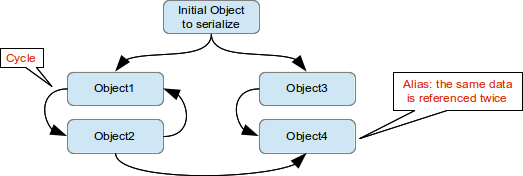
\includegraphics{images/object_graph.png}
\caption{An object graph that contains a cycle and a alias. Cycles must be detected to prevent the serialization algorithm from looping ; aliases must be detected to prevent duplication of the same object.}
\label{object_graph}
\end{figure}

\paragraph{Dynamic reading} Dynamically typed languages do not mandate checks for data integrity before use. Typically, dynamic programmers try to apply methods and are satisfied when the program does not crash ; that is the duck typing philosophy: "When I see a bird that walks like a duck and swims like a duck and quacks like a duck, I call that bird a duck\footnote{James Whitcomb Riley}.". Below we propose a Python code that creates two classes \ipython{Duck} and \ipython{Person} that share some methods in common:
\begin{python}
class Duck:
	def walk(self):
		print "Walk like a duck."
	def swim(self):
		print "Swim like a duck."
	def quack(self):
		print "Quaaaaaack!!!"

class Person:
	def walk(self):
		print "Walk like a baoss!"
	def swim(self):
		print "Swim like a baoss!"

duck = deserialize()
duck.walk()
duck.swim()
duck.quack()
\end{python}
In the case \ipython{deserialize()} returned an instance of the \ipython{Person} class, we get a very late error detection:
\begin{shell}
Walk like a baoss!
Swim like a baoss!
AttributeError: Person instance has no attribute 'quack'
\end{shell}
The drawback of duck typing is the late error detection when data type are confused. For instance, lets say that a biologist reads gigabytes of data and assumes he received back a DNA object when he actually got a RNA object. Because those objects are very similar, he may use the RNA as a DNA for a while in a lot of very expansive computations without crashing the application. So this type error may be detected very late which will result in a great time loss for our biologist. Or even worse, the type error may not be detected at all leading to erroneous results.

\paragraph{Static reading} On the other hand, most static programming patterns force to check data integrity as soon as possible. Those patterns usually catch erroneous input right after the deserialization. Static reading is much safer than dynamic reading but it supposes the programmer is aware of the type system and wants to spend time coding data integrity checks which may not be the case for our stressed biologist. In Java, objects can be serialized when they implement the \ijava{Serializable} interface. In that case, we can serialize and deserialize objects using respectively the methods \ijava{readObject} and \ijava{writeObject} on an \ijava{ObjectInputStream} instance. The result of \ijava{readObject} is an object and it needs to be cast before use. Below, we attempt to deserialize a banana object from a file named \icode{banana.ser} for eating purposes:
\begin{java}
try {
	ObjectInputStream ois = new ObjectInputStream(new FileInputStream("banana.ser"));
	Object o = ois.readObject();
	Banana b = (Banana) o;
	b.eat();
	ois.close();
} catch(Exception e) {
	e.printStackTrace();
}
\end{java}
In case a \ijava{Banana} has not been deserialized, the casts \ijava{(Banana) o} would throw a runtime cast exception. By testing data integrity right after deserialization, we can avoid needless computations.

\paragraph{Context-aware reading} If the reading method is aware of the type the invoker expects, type errors can be detected even during the deserialization. In that case the method can perform a sort of lazy reading where type related information is loaded before the whole parsing. For instance, lets suppose a biologist uses the following Scheme library to work with DNA and RNA objects:
\begin{scheme}
;; DNA constructors
(define (DNA-from-sequence seq) ...)
(define (DNA-from-input in) ...)

;; RNA constructors
(define (RNA-from-sequence seq) ...)
(define (RNA-from-input in) ...)

;; tells if the input represents a DNA or a RNA
(define (read-type input) ...)

;; reads the input ; no guarantee on the result type
(define (unsafe-read input)
  (let ((type read-type))
    (cond ((equal? type DNA) (DNA-from-input input))
          ((equal? type RNA) (RNA-from-input input))
          (else (error "unknown type")))))

;; read the input ; if the call succeeds, the result is of type <expected-type>
(define (safe-read input expected-type)
  (if (equal? (read-type input) expected-type)
      (unsafe-read input)
      (error "the input has the wrong type")))

;; complement makes sens for DNAs and RNAs
(define (complement x) ...)

;; find-sequence makes sens only if x and y are both DNA or bot RNA
(define (contain? x y) ...)
\end{scheme}
Type information inside the serialization format need to be quickly accessible in order to decrease the computation time of \ischeme{read-type}. The following XML sample \ixml{<DNA>AGCTTT...GG</DNA>} is a reasonable format. This library proposes two ways to deserialize DNA/RNA structures:
\begin{enumerate}
\item \emph{Unsafe way}: potential type errors are detected after a lot of unnecesarry computations: 
\begin{scheme}
(define (unsafe-computation input)
  (let ((x (unsafe-read input)))               ;; no guarantee about the type of x
    (complement x)                             ;; expensive computation
    ...                                        ;; expensive computations
    (contain? x (DNA-from-sequence "AAGTTC"))) ;; unsafe call, x may be an RNA
  "end")
\end{scheme}
\item \emph{Context-aware way}: potential type errors are detected as soon as possible inside the reading method:
\begin{scheme}
(define (safe-computation input)
  (let ((x (safe-read input DNA)))             ;; x is guaranteed to be a DNA
    (complement x)                             ;; expensive computation
    ...                                        ;; expensive computations
    (contain? x (DNA-from-sequence "AAGTTC"))) ;; safe call, x is a DNA
  "end")
\end{scheme}
\end{enumerate}

\paragraph{Iterative reading} Using iterative typing, the unsafe use is actually equivalent to the safe use ; guards are automatically inserted. Indeed iterative typing can deduce that the second branch of \ischeme{unsafe-read} is not viable inside the polymorphic call \ischeme{(let ((x (unsafe-read input))) ...)} \reffig{dna_annotated}.
\begin{enumerate}
\item From the body of \ischeme{DNA-from-sequence}, its type is inferred to $String \to DNA$.
\item (1) implies that \ischeme{(DNA-from-sequence "AAGTTC")} is of type $DNA$.
\item From the body of \ischeme{contain?}, its type is inferred to $\forall a . (a,a) \to Boolean$.
\item (2) and (3) imply that the variable \ischeme{x} must also contain a value of type $DNA$.
\item (4) implies that \ischeme{(unsafe-read input)} must be of type $DNA$.
\item From the body of \ischeme{RNA-from-input}, its type is inferred to $String \to RNA$.
\item (5) and (6) implies that the second conditional branch is not viable because it returns a $RNA$ when a $DNA$ is required by the invoker.
\end{enumerate}
As a result, if the input represents a RNA, the application will raise an error right after the predicate evaluation \ischeme{(equal? type "RNA")} and not at the very end of the program. The user of the library does not have to care about types and still can produce applications that catch errors very early. This scenario was the motivating case for the iterative typing development. The attentive reader may try to reproduce the demonstration \reffig{dna_annotated} from the below LScheme code:
\begin{scheme}
;; DNA-from-sequence :: String -> DNA 
(define (DNA-from-sequence seq) ...)
;; DNA-from-input :: String -> DNA
(define (DNA-from-input in) ...)

;; DNA-from-sequence :: String -> RNA
(define (ARN-from-sequence seq) ...)
;; DNA-from-input :: String -> RNA
(define (RNA-from-input in) ...)

;; read-type :: String -> String
(define (read-type input) ...)

;; unsafe-read :: \-/ a . String -> a
(define (unsafe-read input)
  (let ((type read-type))
    (cond ((equal? type "DNA") [a => DNA] (DNA-from-input input))
          ((equal? type "RNA") [a => RNA] (RNA-from-input input))
          (else (error "unknown type")))))

;; complement :: \-/ b . b -> b
(define (complement x)
  ...)

;; find-sequence :: \-/ c . (c,c) -> Boolean 
(define (contain? x y)
  ...)

;; unsafe-computation :: String -> String
;; x :: d
(define (unsafe-computation input)
  (let ((x ((sub [a => d] unsafe-read) input)))
    ((sub [b => d] complement) x)
    ...
    ((sub [c => d, c => DNA] contain?) x (DNA-from-sequence "AAGTTC"))
    "end))"
\end{scheme}

\begin{figure}
\centering
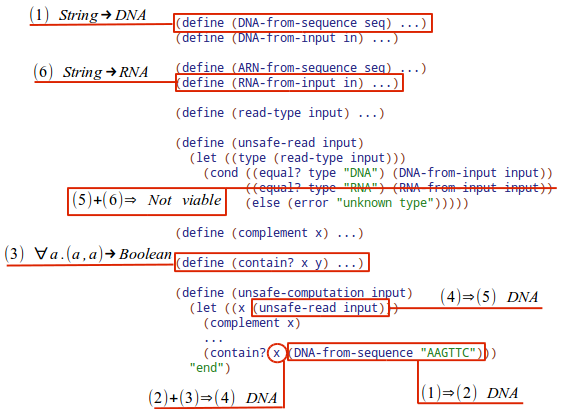
\includegraphics{images/dna_annotated.png}
\caption{Succession of type deductions that demonstrates that the second conditional branch of the polymorphic procedure \ischeme{unsafe-read} is not viable inside the call \ischeme{(let ((x (unsafe-read input)))...)}. That call expects a \ischeme{DNA} as result, not a \ischeme{RNA}.}
\label{dna_annotated}
\end{figure}

\paragraph{A real life example} SBML stands for "Systems Biology Markup Language" it is an XML-like language that is used to encode biologic reactions. SBML provides a real world example of large size objects that are serialized in form where type informations are easily accessible. Indeed SBML documents may be very large and even contain references to biologic data base to load complicated protein structures. Nevertheless very early in the model description, one can define the attribute \icode{id} of the tag \icode{mode} that can be used to predict the kind of model the SBML document describes. Below, we give a cut example of a SBML document exposed inside the official documentation\cite{sbml}:
\begin{code}
<?xml version="1.0" encoding="UTF-8"?>
<sbml xmlns="http://www.sbml.org/sbml/level3/version1/core" level="3" version="1">
	<!-- The model represented by this document is dimerization -->
	<model id="dimerization" substanceUnits="item" timeUnits="second"
	                         volumeUnits="litre" extentUnits="item">
		<listOfUnitDefinitions>
		...
		</listOfUnitDefinitions>
		<listOfCompartments>
		...
		</listOfCompartments>
		<listOfSpecies>
		...
		</listOfSpecies>
		<listOfReactions>
		...
		</listOfReactions>
	</model>
</sbml>
\end{code}
The reading procedure for SBML documents would have the following form in LScheme:
\begin{scheme}
;; readSBML :: \-/ a . string -> a
(define (readSBML docSBML)
  (let (id ((getSBML "model" "id" docSBML)))
    (cond ([a => facilitated_ca_diffusion] (equal? id "facilitated_ca_diffusion") ...)
          ([a => lotkaVolterra_tranport]   (equal? id "lotkaVolterra_tranport")   ...)
          ([a => dimerization]             (equal? id "dimerization")             ...)
          ([a => String]                   else                    "Unknown model"))))
\end{scheme}
As for the DNA-RNA case, type errors would be detected right inside the reading procedure at the case analysis.

\section{Computation context}

\paragraph{Introduction} Sometimes values alone do not suffice to represent the result of a computation. Additional informations, called computation context, may be needed to precisely define how the computation happened. One evident context is the failure context that indicates the computation did not end properly. But other contexts may be useful like confidence indices, relative errors, etc. When those contexts are represented by different types, iterative typing can detect very early the production of a wrong context.

\paragraph{Failure context} When a computation cannot be performed normally, the failure can be handled with different patterns:
\begin{enumerate}
\item \emph{Error marker}: when the procedure detects an illegal configuration it directly returns a marker that must be interpreted as a failure. This is the old-fashion error handling where the invoker must systematically test the result to verify the computation succeed. In case of failure the invoker may either handle it or return an error marker. The following Java code illustrates such pattern with the classic division by zero error:
\begin{java}
// code error for division by zero
static double DIVISION_BY_ZERO = Double.MIN_VALUE;
	
// divide performs an integer division
// It fails when it receives 0 as divisor
public static double integerDivision(int x, int y) {
	if (y == 0) {
		return DIVISION_BY_ZERO;
	} else {
		return x / y;
	}
}

// randomDivision lets the invoker handle the division by zero case
public static double randomDivision() {
	Random r = new Random();
	int x = r.nextInt();
	int y = r.nextInt();
	return integerDivision(x,y);
}

// safeMain handles the potential division by zero
public static void safeMain() {
	double d = randomDivision();
	if (d == DIVISION_BY_ZERO) {
		System.out.println("Unfortunately 0 has been picked as a divisor");
	} else {
		System.out.println(2 * d);
	}
}

// unsafeMain return an inconsistent result in division by zero case
public static void unsafeMain() {
	System.out.println(2 * randomDivision());
}
\end{java}
Lets notice that in statically typed languages there is no clear distinction between the error marker and regular return values since they must share the same type. In consequence, the error marker could be confused with a correct result.
\item \emph{Exceptions}: high level languages usually propose native structures to handle errors. Here, we present the exception handling proposed by Goodenough\cite{exception} which is very common. Semantically, this pattern is mainly equivalent to the error marker one but facilities are provided to separate exceptions generation from exceptions handling. The following Java code performs the same actions as the first one but in a more concise and elegant way:
\begin{java}
// divide fails if it receives 0 as divisor.
public static int integerDivision(int x, int y) throws ArithmeticException {
	if (y == 0) {
		throw new ArithmeticException();
	} else {
		return x / y;
	}
}

// randomDivision lets the invoker handle division by zero cases
public static int randomDivision() throws ArithmeticException {
	Random r = new Random();
	int x = r.nextInt();
	int y = r.nextInt();
	return integerDivision(x,y);
}

// main handle the potential division by zero
public static void safeMain() {
	try {
		System.out.println(2 * (randomDivision()));
	} catch (ArithmeticException e) {
		System.out.println("Unfortunately 0 has been picked as a divisor");
	}
}

// uncaught exception that may cause the application to stop
public static void unsafeMain() throws ArithmeticException {
	System.out.println(2 * (randomDivision()));
}
\end{java}
\item \emph{Persistent computation}: to conserve library use as simple as possible, some languages like Matlab often return usable result in case of failure. For instance \imatlab{1/0} in the Matlab console gives \imatlab{Inf} which can be used as a number.
\end{enumerate}

\paragraph{Iterative marker} Currently iterative typing does not support exceptions. Nevertheless the marker pattern can be implemented very successfully. Thanks to dynamic conditional structures the type of the error marker may be different from the one of the regular values. That way, the use of the marker will produce a type error instead of an inconsistent result. As usual that error will be detected as soon as the failure is detected by the dynamic conditional structure:
\begin{scheme}
;; return null in division by zero case
(define (division x y)
  (if (= y 0)
      "division by zero" ; error detection on unsafe use
      (/ x y)))

;; let the invoker handle the division by zero case
(define (randomDivision)
  (define x (randomNumber))
  (define y (randomNumber))
  (division x y))

;; handle the division by zero case
(define (safe-main)
  (define x (randomDivision))
  (if (null? x)
      (display "Unfortunately 0 has been picked as a divisor")
      (display (* 2 x))))

;; force randomDivision to return a number
(define (unsafe-main)
  (define x (randomDivision))
  (display "dummy string")
  (display (* 2 x)))
\end{scheme}
\begin{enumerate}
\item \emph{Scheme execution}: in case of division by zero, a type error is raised at \ischeme{* 2 x} which is still better than displaying an inconsistent result:
\begin{shell}
dummy string
*: expects type <number> as 2nd argument, given: null; other arguments were: 2
\end{shell}
\item \emph{Iterative execution}: in case of division by zero, a type error is raised right after failure detection at the conditional structure of \ischeme{division} ; we get:
\begin{shell}
Unification failed on [String => Number]
\end{shell}
\end{enumerate}

\paragraph{Marker-Persistent pattern} Iterative typing allows to combine the persistent computation and the error marker pattern through the \ischeme{if-viable} experimental feature. \ischeme{(if-viable <attempt> <alt>)} only executes \ischeme{<attempt>} when it is viable according to iterative typing. 
\begin{scheme}
(if-viable <attempt>
           <alt>)
;; Semantically equivalent ;; 
(if <attempt viable?>
    <attempt>
    <alt>)
\end{scheme}
The procedure that detects an error can, thanks to \ischeme{if-viable}, know if the error marker will be handled or if it will produce a type error later on. Knowing this, it may want to adjust its strategy and return a usable result instead to prevent the whole application to stop:
\begin{scheme}
;; create-matrix :: [[Number]] -> Matrix
(define (create-matrix s) ...)

;; det :: Matrix -> Number 
(define (det m) ...)

;; add-matrix :: (Matrix,Matrix) -> Matrix
(define (add-matrix m1 m2) ...)

;; inv :: \-/ a . Matrix -> a
(define (inv m)
  (if (= (det m) 0)
      (if-viable "zero determinant"
                 infinite-matrix)
      <matrix inversion>))

;; safe :: Matrix -> String
(define (safe m)
  (define inv-m (inv m))
  (if (string? inv-m)
      (display inv-m)
      (display (add-matrix inv-m m)))
  "end")

;; unsafe :: Matrix -> String
(define (unsafe m)
  (display (add-matrix (inv m) m))
  "end")
\end{scheme}
\begin{enumerate}
\item \emph{Safe use}: because \ischeme{safe} tests the result of \ischeme{inv}, the \ischeme{inv} procedure detects that is has been call in a safe context. In the invoker handles the error marker pattern, \ischeme{inv} can safely return the null pointer:
\begin{shell}
> (safe (create-matrix (list (list 1 2 3) (list 1 2 3) (list 4 5 6))))
"m cannot be inversed"
\end{shell}
\item \emph{Unsafe use}: because \ischeme{unsafe} does not test the result of \ischeme{inv} before calling \ischeme{add-matrix}, the \ischeme{inv} procedure detects that it has been called in an unsafe context. In that case, \ischeme{inv} knows that returning \ischeme{null} will produce a type error and that the invoker did not implement the error marker pattern. As a result the persistent computation pattern is used:
\begin{shell}
> (unsafe (create-matrix (list (list 1 2 3) (list 1 2 3) (list 4 5 6))))
[Inf Inf Inf, Inf Inf Inf, Inf Inf Inf]
\end{shell}
\end{enumerate}
We highlight the point that all the consequences of the \ischeme{inspect} special form have not been investigated so far ; a more elaborate presentation of \ischeme{inspect} can be found at \refch{ch_future}.

\section{Side effects}

The leitmotiv of iterative typing is to detect errors earlier without changing the Scheme semantic. This is a praise-worthy goal but detecting errors earlier may actually modify the semantic if we consider side effects.

\paragraph{Side effects} A procedure is said to have side effects when it can interact with the outside world with other means than its result. Below we give an implementation of the map procedure, this procedure is free of side effect ; its result has to be used otherwise the computation is useless:
\begin{scheme}
(define (map f xs)
  (if (null? xs)
      null
      (cons (f x) (map f (cdr xs)))))
      
(begin
  (map (lambda (x) (+ x 1)) (list 1 2 3)) ; useless computation
  "done")
\end{scheme}
Below we give the definition of a procedure that computes the square of its argument and stores the result inside the variable \ischeme{*global*}:
\begin{scheme}
(define *global* null)
(define (side-effect-square x)
  (set! *global* (* x x))
  "done")

(begin
  (side-effect-square 2) ; usable computation result can be retrieved 
  "done")
\end{scheme}
In this section we make a distinction between internal side effects that are cleared when the application exits and external side effects that remain after the application exits. Internal side effects are mainly represented by assignments like \ischeme{set!}. External side effects may involve the file system or the console with \ischeme{display}.

\paragraph{Semantic modification} By detecting errors earlier, iterative typing also stops the program earlier. This may prevent some side effects to happen:  
\begin{scheme}
(define (launch-da-rocket x)
  (if <pred>
      (begin
        ...
        (display "Launch da rocket!!!")
        ...
        (+ x 1))
      <alt>))
(launch-da-rocket "foo")                  
\end{scheme}
\begin{enumerate}
\item \emph{Scheme execution}: when the above program is executed by a standard Scheme interpreter, the rocket is launched then the application raises a type error:
\begin{shell}
Launch da rocket!!!
+: expects type <number> as 1st argument, given: "foo"; other arguments were: 1
\end{shell}
\item \emph{LScheme execution}: when the above program is executed by an iterative Scheme interpreter, the application raises the type error before launching any rocket:
\begin{shell}
Unification failed on [String => Number]
\end{shell}
\end{enumerate}
Notice that internal side effects are not concerned by this discussion since the application will exits anyway. As exposed below, this semantic variation may have good and bad implications.

\paragraph{Positive scenario} Many processes may leave the computer in an undesirable state if not terminated properly. This is the case for resource allocation, a common pattern when several instances want to manipulate the same data:
\begin{enumerate}
\item The instance waits its turn to use the resource.
\item When the instance obtains the permission, it is the only one allowed to manipulate the resource.
\item Once its job on the resource is done, the instance releases the resource to allow another instance to use the resource.
\end{enumerate}
If the resource is not released, other instances may never access it which can be catastrophic. Below we present a Scheme code where iterative early error detections allow to prevent the resource to be locked for ever:
\begin{scheme}
(define (write x)
  (if <pred>
      (begin                             ; LScheme error detection
        (display "lock resource")
        (write resource (concat x "yo")) ; Scheme error detection
        (display "unlock resource"))
      <alt>))
(write 1)
\end{scheme}
\begin{enumerate}
\item \emph{Scheme execution}: the permission has been aquired ; after the application exits, the resource cannot be manipulated anymore:
\begin{shell}
lock resource
concat: expects type <string> as 1st argument, given: 1; other arguments were: "yo"
\end{shell}
\item \emph{LScheme execution}: the permission has not been acquired ; after the application exits, the resource may still be manipulated:
\begin{shell}
Unification failed on [String => Number]
\end{shell}
\end{enumerate}

\paragraph{Negative scenario} Even if it seems natural to decrease the impact of a program that will crash anyway, sometimes we do want to execute the program as far as possible. For instance, programmers typically use log files to debug application. Those files contain information about the program execution and it is bad if some traces are missing. Iterative typing may reduce the amount of provided information: 
\begin{scheme}
(define (write-log x)
  (if <pred>
      (begin                                  ; LScheme error detection
        (write "Log start")
        ...
        (write (concat "x is a" (type-of x)))
        (write (concat x "yo"))               ; Scheme error detection
        ...)
      <alt>))
\end{scheme}

\paragraph{"Unsafe" saves the day} The above scenario demonstrates that it can be useful to grant programmers the ability to shut down iterative typing for a while. This has been achieved with the implementation of the \ischeme{(unsafe <body>)} special form ; if a type error is detected early inside \ischeme{<body>} the iterative prediction is switched off instead of raising an error. As a result, LScheme execution inside the \ischeme{unsafe} special form has the same semantics as the pure Scheme execution:
\begin{scheme}
(define (launch-rocket x y)
  (if x
      (begin (display "Launch rocket!!!")
             (+ x 1))
      (concat x "foo")))
\end{scheme}
\begin{enumerate}
\item \emph{LScheme execution}: the application crashes before launching any rocket:
\begin{scheme}
(launch-rocket #t "bar")
\end{scheme}
\begin{shell}
Unification failed on [String => Number].
\end{shell}
\item \emph{Unsafe execution}: the rocket is launched before the application crashes ; the error is caught by the underlying Scheme instead of the iterative interpreter:
\begin{scheme}
(unsafe (launch-rocket #t "bar"))
\end{scheme}
\begin{shell}
"Launch rocket!!!"
+ expects type <number> of as 1st argument, given: "bar"; other arguments were: 1
\end{shell}
\end{enumerate}

\paragraph{Recapitulation} The combination of early error detection and external side effects cause iterative typing to modify the original Scheme semantic. In some cases, this can be an issue and that is why iterative typing provides the \ischeme{unsafe} special form that allows to shut down early error detection and to execute code with the exact Scheme semantic.

\section{Conclusion}

In this chapter we saw three case studies. The first case study is about early error detection for deserialization patterns. The second case study exhibits how iterative typing can implement a mix of marker and persistent patterns for exceptions management. The last case study is a discussion about early error detection and side effect. The second case study is an application of the \ischeme{if-viable} special form and the third case study is an application of the \ischeme{unsafe} special form. Those case studies highlight the fact that iterative typing completely hides the type complexity from the programmer. As a result, very unskilled programmers can implement relatively safe dynamic programs. A part of the scientific community uses dynamic languages to easily develop applications, those scientists could use iterative typing as a mean to detect errors earlier without changing theirs habits.

%%%%%%%%%%%%%%%%%%%%%%%%%%%%%%%%%%%%%%%%
%%%%%%%%%%%%%%%%%%%%%%%%%%%%%%%%%%%%%%%%
%%%%%%%%%%%%%%%%%%%%%%%%%%%%%%%%%%%%%%%%
%%%%%%%%%%%%%%%%%%%%%%%%%%%%%%%%%%%%%%%%
\chapter{Theoretical basis\label{ch_theory}}
%%%%%%%%%%%%%%%%%%%%%%%%%%%%%%%%%%%%%%%%
%%%%%%%%%%%%%%%%%%%%%%%%%%%%%%%%%%%%%%%%
%%%%%%%%%%%%%%%%%%%%%%%%%%%%%%%%%%%%%%%%
%%%%%%%%%%%%%%%%%%%%%%%%%%%%%%%%%%%%%%%%

At this point, the reader must have a precise idea about what iterative typing is capable of and some intuition about how it is implemented. The first part of this chapter provides a strong base for iterative typing. The second part goes deep down the iterative typing implementation and, according the theoretical base, justify most implementation choices.

\section{Type set}

In this section we introduce very standard concepts \cite{hm1}\cite{grad1}\cite{soft1} that will be used in the entire chapter.

\paragraph{Monotypes} The monotype set is an infinite set based on type variables and type constructors. We use $\tau$, $\xi$, $\gamma$ to respectively range over monotypes, type variables and type constructors. A monotype is either a type variable or a constructed type ; formally the type set is recursively defined as $\tau = \xi\ |\ \gamma\ \tau\ \ldots\ \tau$. A common interpretation of type variable is that they can represent any type. Type constructors accept a fixed number of monotype, this number being the arity of the type constructor, and return a new kind of monotype.

\paragraph{Primitive type} Zero-arity type constructors construct primitive types. Each primitive type represents a set of semantic values whose elements can be represented as constants inside a program. The primitive types we will use are $String$, $Boolean$ and $Number$. We assume the existence of a function $typeOf$ that returns the primitive type of the given constant:
\begin{itemize}
\item $typeOf("foo")=String$
\item $typeOf(123)=Number$
\end{itemize}

\paragraph{Compound type constructors} Those type constructors expect at least one monotype to construct new kind of types. By referencing other monotypes those constructors can be nested without theoretical limit:
\begin{enumerate}
\item \emph{Functional type constructor}: Values of type $\tau\to\tau'$ are procedures that, once they get a value of type $\tau$, returns value of type $\tau'$. For simplicity reasons, in this part of the thesis we will consider that procedures exactly accept one single argument ; so the arity of $\to$ is exactly two. Nevertheless we will see that this restriction does not reduce the expressive power of the language. Here are a bunch of $\lang$ procedure definitions with one of their associated type:
\begin{itemize}
\item $(\lambda\ x\ (if (<\ x\ 0)\ "pos"\ "neg"))\ :\ Number\to String$
\item $(\lambda\ x\ x)\ :\ \xi\to\xi$
\item $(\lambda\ f\ (f\ "foo"))\ :\ (String\to\xi)\to\xi$
\end{itemize}
\item \emph{List type constructor}: values of type $[\tau]$ are lists whom each element is of type $\tau$. Here is some $L$ expressions that return lists:
\begin{itemize}
\item $(list\ 1\ 2\ 3)\ :\ [Number]$
\item $(cons\ "foo"\ (cons\ "bar"\ null))\ :\ [String]$
\end{itemize}
\item \emph{Pair type constructor}: values of type $(\tau_1.\tau_2)$ are pairs whom first element is of type $\tau_1$ and whom second element is of type $\tau_2$. Here is some $L$ expressions that return lists:
\begin{itemize}
\item $(pair\ 1\ "foo")\ :\ (Number.String)$
\item $(pair\ (pair\ 1\ "bar")\ 2)\ :\ ((Number.String).Number)$
\end{itemize}
\end{enumerate}

\paragraph{Polytypes} Polytypes are monotypes whose some type variables have been linked ; we use $\sigma$ to range over the set of polytypes. The formal recursive definition of the polytypes is: $\sigma=\tau\ |\ \forall\xi.\tau$. Polytypes introduce the concept of scoping for type variables ; for instance in the polytype: $\forall \xi.\xi\to Number$, outside $\xi$ are dissociated from the inside $\xi$ that appear in $\xi\to Number$. Below, we give some examples of expressions with their polytype:
\begin{itemize}
\item $(\lambda\ x\ x)\ :\ \forall\xi.\xi\to\xi$
\item $(\lambda\ f\ (f\ 1))\ :\ \forall\xi.(Number\to\xi)\to\xi$
\item $(\lambda\ f\ (\lambda\ x\ (f\ x)))\ :\ \forall\xi_1,\xi_2.((\xi_1\to\xi_2)\to\xi_1)\to\xi_2$
\end{itemize}
$\forall\xi_1,\xi_2,\ldots.\tau$ is an abusive notation to denote $\forall\xi_1.\forall\xi_2.\ldots.\tau$.

\paragraph{Free type variables} Informally, the free type variables of a type represent the type variables that appear inside the type but are not linked to it:
$$\left\{\begin{array}{l}
free(\xi)=\{\xi\}\\
free(\gamma\ \tau_1\ \ldots\ \tau_k)=\bigcup_{i=1}^k{free(\tau_i)}\\
free(\forall\xi.\sigma)=free(\sigma)-\{\xi\}\\
\end{array}\right.$$
Here are the free variable sets of some types:
\begin{itemize}
\item $free(\forall\xi.\xi\to\xi')=\{\xi'\}$
\item $free(\forall\xi.\xi')=\{\xi'\}$
\item $free(\forall\xi.String\to\xi)=\{\}$
\item $free(\xi\to String)=\{\xi\}$
\end{itemize}

\paragraph{Instantiations} Instantiations are mappings from type variables to monotypes written $[\xi_i\mapsto\tau_i]$. The mapping only affects the free type variables of a type. Two examples of instantiation are given below:
\begin{itemize}
\item $\left[\xi\mapsto String\right]\xi\to\xi=String\to String$
\item $\left[\xi_1\mapsto(\xi\to String), \xi_2\mapsto Number\right]\xi_1\to(\xi_2\to Boolean)=(\xi\to String)\to (Number\to Boolean)$
\item $\left[\xi_1\mapsto String,\xi_2\mapsto Number\right]\forall \xi_1.\xi_1\to\xi_2=\forall\xi_1.\xi_1\to Number$
\end{itemize}

\paragraph{Equivalence} The equivalence on monotype is reduced to the syntactical identity. That is: two monotypes are equivalent if and only if their symbolic representation is identical. The equivalence on polytype is a little bit more elaborated. Basically polytype equivalence is similar to the syntactical equivalence up to the name of the linked type variables. Again we skip the formal definition and simply provide some examples:
\begin{itemize}
\item $\xi\to String = \xi\to String$
\item $\xi_1\to String \neq \xi_2\to String$
\item $\forall\xi_1.\xi_1\to String = \forall\xi_2.\xi_2\to String$
\end{itemize}

\paragraph{Subtype partial order} We do not defined any order relation on types ; as a result, given two types we can only say if they are equivalent or not. On the other hand, we do provide a partial order relation for type schemes. Intuitively, the partial order $\sqsubseteq$, named subtype relation\footnote{The reader should not confuse this relation with the concept of subtyping in object oriented paradigm ; here subtyping is used in the sens of \cite{grad3}}, ranks type schemes following their specificity. Formally $\sigma$ is a subtype of $\sigma'$ means that it exists an instantiation on $\sigma'$ linked type variables that unifies the type part of $\sigma$ and $\sigma'$:
$$\left\{\begin{array}{l}
\forall \xi
\sigma\sqsubseteq\forall\xi.\sigma'\Leftrightarrow(\sigma = \forall\xi.\sigma')\vee(\exists[\xi\mapsto\tau].\sigma\sqsubseteq[\xi\mapsto\tau]\sigma')\\
\sigma\sqsubseteq\tau\Leftrightarrow\sigma=\tau\\
\end{array}\right.$$
As $\sqsubseteq$ is not complete partial order, many type scheme pairs like $\forall \xi.\xi\to String$ and $\forall\xi.\xi\to String$ are not comparable. Here are some examples:
\begin{itemize}
\item$\xi\to String \sqsubseteq \xi\to String$
\item$\forall\xi.\xi\to\xi\sqsubseteq Number\to Number$
\item$\forall\xi.\xi\to\xi\sqsubseteq \xi\to\xi$
\end{itemize}

\paragraph{Alpha-renaming} This technique has been took from the lambda calculus. Alpha renaming is about avoiding name collision by renaming linked variables. After alpha-renaming, we can say that two variables denote the same entity if and only if they share the same name. Below, we present some alpha-renaming:
\begin{itemize}
\item $\forall\xi.\forall\xi.\xi\to String\xlongrightarrow{\alpha} \forall\xi_1.\forall\xi_2.\xi_2\to String$
\item $(\forall\xi.\xi\to\xi_1,\forall\xi.\xi_1\to\xi)\xlongrightarrow{\alpha}(\forall\xi_2.\xi_2\to\xi_1,\forall\xi_3.\xi_1\to\xi_3)$
\end{itemize}

\paragraph{Recapitulation} The different type sets are summarized in \reftab{type_recap}. We then saw the following concepts for type schemes:
\begin{itemize}
\item Free variables, $free(\sigma)$: links capture type variables.
\item Instantiation, $\left[\xi_i\mapsto\tau_i\right]\sigma$: mapping of the free type variables contained in $\sigma$.
\item Equivalence, $\sigma_1 = \sigma_2$: syntactic equivalence up to the symbols used for the linked variables.
\item Subtype relation: $\sigma_1\sqsubseteq\sigma_2$: require equivalence after instantiation of some of $\sigma_2$ linked type variables.
\item Alpha renaming: by renaming the linked variables of type schemes we can avoid name collisions.
\end{itemize}

\begin{table}
\centering
\begin{tabular}{cccc}
\begin{tabular}{|r|l|}
\hline
\multicolumn{2}{|c|}{Primitive types ($I$)}\\
\hline
\hline
$\iota$ & $Boolean$\\
& $Number$\\
& $String$\\
\hline
\end{tabular}
&
\begin{tabular}{|r|l|}
\hline
\multicolumn{2}{|c|}{Monotypes ($M$)}\\
\hline
\hline
$\tau$ & $\iota$\\
& $\xi$\\
& $\tau\to\tau$\\
& $[\tau]$\\
& $(\tau.\tau)$\\
\hline
\end{tabular}
&
\begin{tabular}{|r|l|}
\hline
\multicolumn{2}{|c|}{Polytypes ($P$)}\\
\hline
\hline
$\pi$ & $\forall\xi.\tau$\\
& $\forall\xi.\pi$\\
\hline
\end{tabular}
&
\begin{tabular}{|r|l|}
\hline
\multicolumn{2}{|c|}{Types ($T$)}\\
\hline
\hline
$\sigma$ & $\tau$\\
& $\forall\xi.\sigma$\\
\hline
\end{tabular}
\end{tabular}
\caption{Given an infinite set of type variable ($X$, ranged with $\xi$) this table defines recursively the sets: primitive types, monotypes, polytypes, and types. The following relation can be easily verified: $I\subset M\subset P\subset T$. Primitives types are the zero arity type constructors. Monotypes are combinations of type constructors and type variables. Polytypes must contain at least one link before their mono-part. The type set is the union of the monotype set and the polytype set.}
\label{type_recap}
\end{table}

\section{The $\lang$ language}

$\lang$ is a representation of an atomic subset of Scheme which is much more suitable to be expressed in type systems. As argued in this section, despite being atomic $\lang$ has about the same expressive power as Scheme without assignments and continuations. The semantic of Scheme will be skipped since it is exposed at \refan{an_scheme}. Because the transformation from atomic Scheme to $\lang$ is exposed in this section, we skip the semantic of $\lang$ as well.

\begin{table}
\centering
\begin{tabular}{|l||r||l||r||l|}
\hline
\multicolumn{1}{|c||}{Name}&\multicolumn{2}{|c||}{Atomic Scheme} & \multicolumn{2}{|c|}{$\lang$}\\
\hline
\hline
Constant&\ischeme{<EXPR>} & \ischeme{c} & $e$ & $c$\\
Identifier && \ischeme{x}& & $x$\\
Abstraction && \ischeme{(lambda (<PARAM>) <EXPR>)}& & $(\lambda\ x\ e)$\\
Application && \ischeme{(<EXPR> <EXPR>)} & & $(e\ e)$\\
Binding && \ischeme{(let ((x <EXPR>)) <EXPR>)} & & $(let\ x\ e\ e)$\\
Conditional structure && \ischeme{(if <EXPR> <EXPR> <EXPR>)} & & $(if\ e\ e\ e)$\\
\hline
\end{tabular}
\caption{The equivalence of each $\lang$ expression in Scheme.}
\label{lang_gramm}
\end{table}

\paragraph{Statement elimination} To keep type systems as simple as possible, we must eliminate the concept of statement. Statements can be easily replaced by nested \ischeme{let} expression:
\begin{itemize}
\item \emph{Definition statement}: Without assignment, removing definition also allow to remove side effect on the environment.
$$\llbracket\ischeme{(define x <bind>) <rest>}\rrbracket=\ischeme{(let ((x }C\llbracket\ischeme{<bind>}\rrbracket\ischeme{)) }C\llbracket\ischeme{<rest>}\rrbracket\ischeme{)}$$
	\begin{itemize}
	\item $C\llbracket\ischeme{(define pi 3.14) (* 2 pi)}\rrbracket=\ischeme{(let ((pi 3.14)) (* 2 pi))}$
	\item $C\llbracket\ischeme{(define pi 3.14) (define e 2.71) (* pi e)}\rrbracket=\ischeme{(let ((pi 3.14)) (let ((e 2.71)) (*\ pi\ e)))}$
	\end{itemize}
\item \emph{Other statement}: Here a dummy name \ischeme{_} is used ; it should never be referenced.
$$C\llbracket\ischeme{<expr> <rest>}\rrbracket=\ischeme{(let ((_ }C\llbracket\ischeme{<expr>}\rrbracket\ischeme{)) }C\llbracket\ischeme{<rest>}\rrbracket\ischeme{)}$$
	\begin{itemize}
	\item $C\llbracket\ischeme{(display "foo") (+ 1 2)}\rrbracket=\ischeme{(let ((_ (display "foo"))) (+ 1 2))}$
	\item $C\llbracket\ischeme{(define pi 3.14) (display "foo") (* 2 pi)}\rrbracket=\ischeme{(let ((pi 3.14)) (let ((_ (display "foo"))) (+ 1 2)))}$
	\end{itemize}
\end{itemize}

\paragraph{Fixing the arity} The second difficulty we prefer to avoid is the freedom about procedure arity. With the fellowing syntactic transformations we can simulate the behavior of multiple argument procedure with only procedure of one argument:
\begin{itemize}
\item \emph{Constant procedure}: This case correspond to the definition of a procedure that takes no arguments. We introduce an artificial argument whose symbol is \ischeme{_} and whose value is a constant of a specific type \ischeme{#_}:
$$\left\{\begin{array}{l}
C\llbracket\ischeme{(lambda () <body>)}\rrbracket=\ischeme{(lambda (_) }C\llbracket\ischeme{<body>}\rrbracket\ischeme{)}\\
C\llbracket\ischeme{(<abs>)}\rrbracket=\ischeme{(}C\llbracket\ischeme{<body>}\rrbracket\ischeme{ #_)}\\
\end{array}\right.$$
	\begin{itemize}
	\item $C\llbracket\ischeme{(lambda () "foo")}\rrbracket=\ischeme{(lambda (_) "foo")}$
	\item $C\llbracket\ischeme{(f)}\rrbracket=\ischeme{(f #_)}$
	\end{itemize}
\item \emph{Single argument procedure}: No syntactic transformation:
$$\left\{\begin{array}{l}
C\llbracket\ischeme{(lambda (x) <body>)}\rrbracket=\ischeme{(lambda (x) }C\llbracket\ischeme{<body>}\rrbracket\ischeme{)}\\
C\llbracket\ischeme{(<abs> <arg>)}\rrbracket=\ischeme{(}C\llbracket\ischeme{<abs>}\rrbracket\ischeme{ }C\llbracket\ischeme{<arg>}\rrbracket\ischeme{)}\\
\end{array}\right.$$
\item \emph{Multiple argument procedure}: Multiple argument procedures can be transformed into nested mono argument procedure ; such transformation is called curryfication:
$$\left\{\begin{array}{l}
C\llbracket\ischeme{(lambda (x1 <tail>) <body>)}\rrbracket=\ischeme{(lambda (x_1) }C\llbracket\ischeme{(lambda (<tail>) <body>)}\rrbracket\ischeme{)}\\
C\llbracket\ischeme{(<abs> <init> <last>)}=\ischeme{(}C\llbracket\ischeme{(<abs> <init>)}\rrbracket\ischeme{ }C\llbracket\ischeme{<last>}\rrbracket\ischeme{)}\\
\end{array}\right.$$
	\begin{itemize}
	\item $C\llbracket\ischeme{(lambda (x1 x2 x3) x3)}\rrbracket=(\lambda\ x_1\ (\lambda\ x_2\ (\lambda\ x_3\ x_3)))$
	\item $C\llbracket\ischeme{(f 1 2 3)}\rrbracket=(((f\ 1)\ 2)\ 3)$
	\end{itemize}
\end{itemize}

\paragraph{Variable shadowing} We suppose the compilation from the atomic Scheme to $\lang$ alpha-renames all the variables so we do not have to care about variable shadowing in $\lang$. Below we give a program that tests if two numbers are divisible:
\begin{scheme}
(define x 10)
(define (divide? (x y)) (= (modulo x y) 0))
(devide? x 5)
\end{scheme}
After compilation we get:
\begin{scheme}
(let ((x1 10))
  (let ((divide? (lambda (x1) (lambda (y)
                               ((= ((modulo x1) y)) 0)))))
    ((divide? x1) 5)))
\end{scheme}

\paragraph{Recapitulation} What we attempt to do here is to split a difficult problem into easier problems. The original problem was to express a type system for Scheme without assignments nor continuations which is quite hard. The equivalent easier problems are compilation from Scheme to $\lang$ and expression of the type system for $\lang$. The $\lang$ language is free of statements, multiple-argument procedure, variable shadowing and syntactic sugar.

\section{Hindely-Milner type system}

In this section we describe a typical type system rule by rule after introducing assumption set, judgment and derivation

\paragraph{Assumptions set} Assumptions, notated $A$, are sets whose elements have the form: $x:\sigma$. In other words, $A$ associate types to identifiers ; it is basically an environment that carries types instead of values. We extend the concept of free variables to assumptions: the set of the free type variables of an assumption set correspond to the union of all the free variable that appear in those assumptions. Formally we have:
$$free(A)=\bigcup_{x_i:\sigma_i\in A}(free(\sigma_i)$$
Below we give some examples of assumptions instantiation: 
\begin{itemize}
\item $free(\{x:\xi_1\to String,y:\xi_2\})=\{\xi_1,\xi_2\}$
\item $free(\{x:\xi_1\to String, y:\forall \xi_2.\xi_2\to String\})=\{\xi_1\}$
\end{itemize}

\paragraph{Judgment} Judgment have the following form: $A\vdash e:\sigma$ which intuitively means that the assumptions $A$ do not contradict that $e$ is of type $\sigma$. Here are some example of judgments that holds:
\begin{itemize}
\item $\{\}\vdash "foo":String$
\item $\{\}\vdash (\lambda\ x\ x):\xi\to\xi$
\item $\{\}\vdash (\lambda\ x\ x):\forall\xi.\xi\to\xi$
\item $\{x:Number\}\vdash (\lambda\ y\ (+\ x\ y)):Number\to Number$
\end{itemize}
We extend the concept of instantiation to judgments: an instantiation on a judgment corresponds to the instantiation on all its types. Here are some judgment instantiations:
\begin{itemize}
\item $\left[\xi\mapsto Number\right]\{x:\xi\to String,y:\xi\}\vdash y:\xi = \{x:Number\to String,y:Number\}\vdash y:Number$
\item $\left[\xi_1\mapsto\xi,\xi_2\mapsto String\right]\{x:\xi_1,y:[\xi_2],z:\forall\xi_1.\xi_1\to\xi_1\}\vdash x:\xi_1=\{x:\xi_1,y:[String],z:\forall\xi_1.\xi_1\to\xi_1\}\vdash x:\xi$
\end{itemize}
Type instantiation on judgment may seem odd for readers used to type system but it will become very handy to describe the iterative type system. In particular, the rule dedicated to conditional structures make heavy use of this instantiation.

\paragraph{Inference rule \& derivation} An inference rules indicates that given some premise schemes the judgment scheme holds:
$$\ax{premise_1}
\ax{...}
\ax{premise_N}
\tric{conclusion}
\drule$$
In the presented type systems premises are either assertions that must be verified either judgments. Derivations are tree of inference rules in which all the leaves are assertions. A judgment holds if and only if it exists a derivation that ends with that judgment. Inference rules are declarative, that is they do not tell how to construct derivations but given a derivations it is trivial to verify if it respects the inference rules.

\paragraph{Leaves} They are only two rules that does not have to be justified by other rules:
\begin{itemize}
\item ID: the type of an identifier is defined by the current assumption set:
$$\ax{x:\sigma\in A}
\LeftLabel{ID}
\unc{A\vdash x:\sigma}
\drule$$
\item CONST: the type of a constant is supposed to be directly deductible through the previously introduced function $typeOf$:
$$\ax{typeOf(c)=\gamma}
\LeftLabel{CONST}
\unc{A\vdash c:\gamma}
\drule$$
\end{itemize}

\paragraph{Procedure type deductions} Two rules are dedicated to handle type deductions that involve procedures:
\begin{itemize}
\item ABS: Given a procedure $(\lambda\ x\ e)$, if the assumption $x:\tau$ allows to deduce $e:\tau'$ that means the procedure will return a value of type $\tau'$ if it receives a value of type $\tau$. This is the intuitive interpretation of $\tau\to\tau'$:
$$\ax{A\cup\{x:\tau\}\vdash e:\tau'}
\LeftLabel{ABS}
\unc{A\vdash(\lambda\ x\ e):\tau\to\tau'}
\drule$$
\item APP: When we give a value of type $\tau'$ to a procedure of type $\tau'\to\tau$ we expect to receive a value of type $\tau$:
$$\ax{A\vdash e:\tau'\to\tau}
\ax{A\vdash e':\tau'}
\LeftLabel{APP}
\bic{A\vdash (e\ e'):\tau}
\drule$$
\end{itemize}
Here is derivation that justifies the judgment $\{\}\vdash((\lambda\ x\ x)\ 1):Number$ with the four rules introduced so far:
$$\ax{x:Number\in\{x:Number\}}
\LeftLabel{ID}
\unc{\{x:Number\}\vdash x:Number}
\LeftLabel{ABS}
\unc{\{\}\vdash(\lambda\ x\ x):Number\to Number}
\ax{typeOf(1)=Number}
\LeftLabel{CONST}
\unc{\{\}\vdash 1:Number}
\LeftLabel{APP}
\bic{\{\}\vdash ((\lambda\ x\ x)\ 1):Number}
\drule$$

\paragraph{Polymorphism support} From here we move away from the $\lambda$ calculus to support polymorphism:
\begin{itemize}
\item GEN: At any time, if the assumptions does not contain the type variable $\xi$ we can generalize the current deduction $A\vdash e:\sigma$ to $A\vdash e:\forall\xi.\sigma$:
$$\ax{A\vdash e:\forall\xi_{1..i}.\tau}
\ax{\xi\notin free(A)}
\LeftLabel{GEN}
\bic{A\vdash e:\forall\xi,\xi_{1..i}.\tau}
\drule$$
\item SUB: this the inverse rule of GEN: at any time we can make the current deduction more specific:
$$\ax{A\vdash e:\sigma}
\ax{\sigma'\sqsubseteq\sigma}
\LeftLabel{SUB}
\bic{A\vdash e:\sigma'}
\drule$$
\end{itemize}

\paragraph{Polymorphic recursive let} There are many ways to introduce recursion, some use the fix point, others use a dedicated rules. We chose to support both polymorphism and recursion through $let$ expressions. Given $(let\ x\ bind\ body)$ the first think to do is to deduce the type of $bind$ with monomorphic recursion. Monomorphic recursion suppose that both $x$ and $bind$ share the same type which can be expressed by the following judgment: $\{x:\tau\}\vdash bind:\tau$. After that deduction, we should generalize the type of $bind$ to $\sigma$ if we want that $x$ appear polymorphically inside $body$. The overall type is given by type deduction of $body$ knowing that $x$ is of type $\sigma$. So the body of a $let$ allows to enter polymorphically into the binding ; once inside the binding, monomorphic recursion is performed.
$$\ax{A\cup\{x:\tau\}\vdash e:\sigma}
\ax{A\cup\{x:\sigma\}\vdash e':\tau'}
\ax{\tau\sqsubseteq\sigma}
\LeftLabel{LET}
\tric{A\vdash (let\ x\ e\ e'):\tau'}
\drule$$

\paragraph{Conditional structure} Both branches are analyzed the same way and must return the same type ; such modus operandi considerably reduces the expressiveness of $\lang$.
$$\ax{A\vdash e:\tau}
\ax{A\vdash e_1:\tau'}
\ax{A\vdash e_2:\tau'}
\LeftLabel{COND}
\tric{A\vdash (if\ e\ e_1\ e_2):\tau'}
\drule$$

\paragraph{Recapitulation }We first defined the concept of assumptions, judgments and derivations. We also exposed a usual type system based on Hindley-Milner work \reftab{hm_ts}.

\begin{table}
\centering
$$\boxed{\begin{array}{c}\begin{array}{cc}
\\
\ax{\{x:\sigma\}\in A}
\LeftLabel{ID}
\unc{A\vdash x:\sigma}
\drule
&
\ax{typeOf(c)=\gamma}
\LeftLabel{CONST}
\unc{A\vdash c:\gamma}
\drule
\\\\\\
\ax{A\cup\{x:\tau\}\vdash e:\tau'}
\LeftLabel{ABS}
\unc{A\vdash(\lambda\ x\ e):\tau\to\tau'}
\drule
&
\ax{A\vdash e:\tau'\to\tau}
\ax{A\vdash e':\tau'}
\LeftLabel{APP}
\bic{A\vdash (e\ e'):\tau}
\drule
\\\\\\
\ax{A\vdash e:\sigma}
\ax{\xi\notin free(A)}
\LeftLabel{GEN}
\bic{A\vdash e:\forall\xi.\sigma}
\drule
&
\ax{A\vdash e:\sigma}
\ax{\sigma'\sqsubseteq\sigma}
\LeftLabel{SUB}
\bic{A\vdash e:\sigma'}
\drule
\end{array}
\\\\\\
\ax{A\cup\{x:\tau\}\vdash e:\sigma}
\ax{A\cup\{x:\sigma\}\vdash e':\tau'}
\ax{\tau\sqsubseteq\sigma}
\LeftLabel{LET}
\tric{A\vdash (let\ e\ e'):\tau'}
\drule
\\\\\\
\ax{A\vdash e:\tau}
\ax{A\vdash e_1:\tau'}
\ax{A\vdash e_2:\tau'}
\LeftLabel{COND}
\tric{A\vdash (if\ e\ e_1\ e_2):\tau'}
\drule
\\\\
\end{array}
}$$
\caption{A Hindley-Milner based type system.}
\label{hm_ts}
\end{table}

\section{The $\lang$ type system}

The complete type system of $\lang$ is shown at \reftab{l_ts}. Many rules remain intact, this section justifies the modifications done on COND and GEN.
\begin{table}
\centering
$$\boxed{\begin{array}{c}\begin{array}{cc}
\\
\ax{\{x:\sigma\}\in A}
\LeftLabel{ID}
\unc{A\vdash x:\sigma}
\drule
&
\ax{typeOf(c)=\gamma}
\LeftLabel{CONST}
\unc{A\vdash c:\gamma}
\drule
\\\\\\
\ax{A_x\cup\{x:\tau\}\vdash e:\tau'}
\LeftLabel{ABS}
\unc{A\vdash(\lambda\ x\ e):\tau\to\tau'}
\drule
&
\ax{A\vdash e:\tau'\to\tau}
\ax{A\vdash e':\tau'}
\LeftLabel{APP}
\bic{A\vdash (e\ e'):\tau}
\drule
\\\\\\
\ax{A\vdash e:\textcolor{red}{\forall \xi_1,\ldots.\tau\to\tau'}}
\ax{\xi\notin free(A)}
\LeftLabel{\textcolor{red}{LGEN}}
\bic{A\vdash e:\forall\xi,\xi_1,\ldots.\tau\to\tau'}
\drule
&
\ax{A\vdash e:\sigma}
\ax{\sigma'\sqsubseteq\sigma}
\LeftLabel{SUB}
\bic{A\vdash e:\sigma'}
\drule
\end{array}
\\\\\\
\ax{A_x\cup\{x:\tau\}\vdash e:\sigma}
\ax{A_x\cup\{x:\sigma\}\vdash e':\tau'}
\ax{\tau\sqsubseteq\sigma}
\LeftLabel{LET}
\tric{A\vdash (let\ e\ e'):\tau'}
\drule
\\\\\\
\ax{A\vdash e:\tau}
\ax{\textcolor{red}{\left[\xi'\mapsto\tau'\right]}A\vdash e':\tau'''}
\ax{\textcolor{red}{\left[\xi''\mapsto\tau''\right]}A\vdash e'':\tau'''}
\LeftLabel{\textcolor{red}{LCOND}}
\tric{A\vdash (if\ e\ e'\ e''):\tau'''}
\drule
\\\\
\end{array}
}$$
\caption{The $\lang$ type system.}
\label{l_ts}
\end{table}

\paragraph{LCOND rule} The iterative LCOND rule is much more permissive than the static one, it summarizes the essence of iterative typing. LCOND rule makes that the type deduction of each branch does not affect each other and the rest of the deduction. Lets analyze two different conditional structures:
\begin{itemize}
\item Conditional branches can return different types. Here is the proof that the classic evil conditional structure, $(if\ x\ 1\ "foo")$, is accepted by the $\lang$ type system:
$$\begin{array}{c}
\ax{x:B\in\{x:B\}}
\LeftLabel{ID}
\unc{\{x:B\}\vdash x:B\bmarker{*}}
\drule
\\\\\\
\ax{typeOf(1)=N}
\LeftLabel{CONST}
\unc{\left[\xi\to N\right]\{x:B\}\vdash 1:\xi\bmarker{**}}
\drule
\\\\\\
\ax{typeOf("foo")=S}
\LeftLabel{CONST}
\unc{\left[\xi\to S\right]\{x:B\}\vdash "foo":\xi\bmarker{***}}
\drule
\\\\\\
\ax{\textcolor{blue}{*}}
\ax{\textcolor{blue}{**}}
\ax{\textcolor{blue}{***}}
\LeftLabel{LCOND}
\tric{\{x:B\}\vdash (if\ x\ 1\ "foo"):\xi}
\drule
\end{array}$$
\item The identifier use can be encapsulated inside each branch. For instance the $\lang$ code $(if\ x\ (incr\ y)\ (length\ y))$ is accepted by the $\lang$ type system. This code, following the value of $x$, either considers $y$ as a number and increments it or considers $y$ as a string and evaluates its length. Here is the proof that this code is accepted by $\lang$ type system:
$$\begin{array}{c}
\ax{x:B\in\{x:B, y:N, incr:N\to N, length:S\to N\}}
\LeftLabel{ID}
\unc{\{x:B, y:N, incr:N\to N, length:S\to N\}\vdash x:B\bmarker{*}}
\drule
\\\\\\
\ax{y:N\in\{x:B, y:N, incr:N\to N, length:S\to N\}}
\LeftLabel{ID}
\unc{\{x:B, y:N, incr:N\to N, length:S\to N\}\vdash y:N\gmarker{(1)}}
\drule
\\\\\\
\ax{incr:N\to N:\{x:B, y:N, incr:N\to N, length:S\to N\}}
\LeftLabel{ID}
\unc{\{x:B, y:N, incr:N\to N, length:S\to N\}\vdash incr:N\to N\gmarker{(2)}}
\drule
\\\\\\
\ax{\textcolor{green}{(1)}}
\ax{\textcolor{green}{(2)}}
\LeftLabel{APP}
\bic{\left[\xi\to N\right]\{x:B, y:\xi, incr:N\to N, length:S\to N\}\vdash (incr\ y): N\bmarker{**}}
\drule
\\\\\\
\ax{y:S\in\{x:B, y:S, incr:N\to N, length:S\to N\}}
\LeftLabel{ID}
\unc{\{x:B, y:S, incr:N\to N, length:S\to N\}\vdash y:S\gmarker{(3)}}
\drule
\\\\\\
\ax{length:S\to N:\{x:B, y:N, incr:N\to N, length:S\to N\}}
\LeftLabel{ID}
\unc{\{x:B, y:S, incr:N\to N, length:S\to N\}\vdash length:S\to N\gmarker{(4)}}
\drule
\\\\\\
\ax{\textcolor{green}{(3)}}
\ax{\textcolor{green}{(4)}}
\LeftLabel{APP}
\bic{\left[\xi\to S\right]\{x:B, y:\xi, incr:N\to N, length:S\to N\}\vdash (length\ y): N\bmarker{***}}
\drule
\\\\\\
\ax{\textcolor{blue}{*}}
\ax{\textcolor{blue}{**}}
\ax{\textcolor{blue}{***}}
\LeftLabel{LCOND}
\tric{\{x:B, y:\xi, incr:N\to N, length:S\to N\}\vdash (if\ x\ (incr\ y)\ (length\ y)):N}
\drule
\end{array}$$
\end{itemize}

\paragraph{Hindley-Milner type variables} When a Hindley-Milner derivation contains free type variables, each instantiation of those type variables applied on that derivation produces a new valid derivation. Below we give a general derivation for the identity procedure and then instantiate its free type variable $\xi$ to $S$:
$$\begin{array}{ccc}
\ax{x:\xi\in\{x:\xi\}}
\LeftLabel{ID}
\unc{\{x:\xi\}\vdash x:\xi}
\LeftLabel{APP}
\unc{\{\}\vdash(\lambda\ x\ x):\xi\to\xi}
\drule
&
\xlongrightarrow{[\xi\mapsto S]}
&
\ax{x:\xi\in\{x: S\}}
\LeftLabel{ID}
\unc{\{x:S\}\vdash x:S}
\LeftLabel{APP}
\unc{\{\}\vdash(\lambda\ x\ x):S\to S}
\drule
\end{array}$$
We can say that the rules of the Hindley-Milner type system consider type variables as marker that can be replaced by any monotype. This status is verified by the Hindley-Milner type inference where type variables represent unspecified type which wait for an instantiation.

\paragraph{Iterative type variables} In the $\lang$ type system, the status of type variable is damaged. In particular, the rule LCOND produces invalid derivations when instantiations are applied on entire derivations. Below, we illustrate this fact with the traditional $(if\ x\ 1\ "foo")$:
$$\begin{array}{c}
\ax{x:B\in\{x:B\}}
\LeftLabel{ID}
\unc{\{x:B\}\vdash x:B}
\ax{typeOf{1}=N}
\LeftLabel{CONST}
\unc{\left[\xi\mapsto N\right]\{x:B\}\vdash 1:\xi}
\ax{typeOf{"foo"}=S}
\LeftLabel{CONST}
\unc{\left[\xi\mapsto S\right]\{x:B\}\vdash "foo":\xi}
\LeftLabel{LCOND}
\tric{\{x:B\}\vdash (if\ x\ 1\ "foo"):\xi}
\drule
\\\\\\
\xlongrightarrow{[\xi\mapsto S]}
\\\\\\
\ax{x:B\in\{x:B\}}
\LeftLabel{ID}
\unc{\{x:B\}\vdash x:B}
\ax{typeOf{1}=N}
\LeftLabel{CONST}
\unc{\{x:B\}\vdash 1:S}
\ax{typeOf{"foo"}=S}
\LeftLabel{CONST}
\unc{\{x:B\}\vdash "foo":S}
\LeftLabel{LCOND}
\tric{\{x:B\}\vdash (if\ x\ 1\ "foo"):S}
\drule
\end{array}$$
The first instantiation is valid for the $\lang$ type system but its instantiation is not because of the judgment $\{x:B\}\vdash 1:S$. So, inside $\lang$ type system, type variables do not longer represent any monotype. Instead, type variables should be considered as an unknown specific types. Above, the judgment $\{x:B\}\vdash (if\ x\ 1\ "foo"):\xi$ should be understand as: "the derivation did not succeed to find the exact type of $(if\ x\ 1\ "foo")$ ; it can be anything". It is interesting to notice how a small modification of the type system radically affects our comprehension of types.

\paragraph{The generalization rule} Due to the new status of type variables, we want to generalize only functional types. Lets analyze the following Scheme code:
\begin{scheme}
(define x (if <pred> 1 "foo"))
(incr x)   ; x must be a number
(length x) ; x must be a string
\end{scheme}
This code obviously contains a static type error since \ischeme{x} can not be a number and a string at the same time. If we do allow generalization on non functional types the type of the expression \ischeme{(if <pred> 1 "foo")} can be inferred to $\forall \xi.\xi$ and the above code will be accepted with two successive instantiation of \ischeme{x}. Here is the undesirable derivation of $A\vdash (if\ x\ 1\ "foo"):\forall\xi.\xi$:
$$
\ax{x:B\in\{x:B\}}
\LeftLabel{ID}
\unc{\{x:B\}\vdash x:B}
\ax{1 :: N}
\LeftLabel{CONST}
\unc{\left[\xi\to N\right]\{x:B\}\vdash 1:\xi}
\ax{typeOf("foo")=S}
\LeftLabel{CONST}
\unc{\left[\xi\to S\right]\{x:B\}\vdash "foo": \xi}
\LeftLabel{LCOND}
\tric{\{x:B\}\vdash (if\ x\ 1\ "foo"):\xi}
\LeftLabel{GEN}
\unc{\{x:B\}\vdash (if\ x\ 1\ "foo"):\forall\xi.\xi}
\drule
$$

\paragraph{Direct context} We already saw that LCOND rule allows to encapsulate type deduction inside conditional branched. In this paragraph we will see that outside world still continue to affect the type deduction inside the conditional branches. If this statement was not verified, the following $\lang$ code $(incr (if\ x\ 1 "foo"))$\footnote{$incr$ denotes the increment procedure which is of type: $Number\to Number$.} would be accepted which is not desirable since the second branch $"foo"$ will always cause a type error. Below, we give a proof by contradiction that judgments of the form $\{incr:N\to N,A\}\vdash (incr\ (if\ x\ 1\ "foo")):N$ can not be derived in the $\lang$ type system:
\begin{enumerate}
\item As the outmost expression is an application we are forced to use the APP rule:
$$\ax{incr:N\to N\in\{incr:N\to N,A\}}
\LeftLabel{ID}
\unc{\{incr:N\to N,A\}\vdash incr:N\to N}
\ax{\{incr:N\to N,A\}\vdash (if\ x\ 1\ "foo"):N}
\LeftLabel{APP}
\bic{\{incr:N\to N,A\}\vdash (incr\ (if\ x\ 1\ "foo")):N}
\drule$$
\item We then have to justify a judgment of the form: $\{incr:N\to N,A\}\vdash (if\ x\ 1\ "foo"):N$. As the outmost expression is a $if$ we are forced to use the LCOND. This rule requires the justification of the following judgments:
\begin{enumerate}
\item $\{incr:N\to N,A\}\vdash x:\tau$
\item $[\xi_i\to\tau_i]\{incr:N\to N, A\}\vdash 1:N$
\item $[\xi_i'\to\tau_i]\{incr:N\to N,A\}\vdash "foo":N$
\end{enumerate}
Lets focus on the third one: it is a constant so we have to use the CONST rule. That rule requires the verification of the assertion $typeOf("foo")=N$ which is false since $"foo"$ is of type string. By contradiction we can deduce judgments of the form $\{incr:N\to N,A\}\vdash (incr\ (if\ x\ 1\ "foo")):N$ can not be derived in the $\lang$ type system.
\end{enumerate}

\paragraph{Remote context} We will now see that type deductions on different conditional branches are independent. As an illustration, we present a program with two sequential conditional structures and its type derivation:
\begin{scheme}
((lambda (x)
   (if y
       (incr x)
       (length x))) (if z
                        1
                        "foo"))
\end{scheme}
$$\begin{array}{c}
\ax{\mbox{Derived on paragraph LCOND rule.}}
\LeftLabel{...}
\unc{\{x:\xi,y:B,z:B,incr:N\to N,length:S\to N\}\vdash (if\ y\ (incr\ x)\ (length\ x)):N}
\LeftLabel{ABS}
\unc{\{y:B,z:B,incr:N\to N,length:S\to N\}\vdash (\lambda\ x\ (if\ y\ (incr\ x)\ (length\ x))):\xi\to N\bmarker{*}}
\drule
\\\\\\
\ax{\mbox{Derived on paragraph LCOND rule.}}
\LeftLabel{...}
\unc{\{y:B,z:B,incr:N\to N,length:S\to N\}\vdash (if\ z\ 1\ "foo"):\xi\bmarker{**}}
\drule
\\\\\\
\ax{\textcolor{blue}{*}}
\ax{\textcolor{blue}{**}}
\LeftLabel{APP}
\bic{\{y:B,z:B,incr:N\to N,length:S\to N\}\vdash ((\lambda\ x\ (if\ y\ (incr\ x)\ (length\ x)))\ (if\ z\ 1\ "foo")):N}
\drule
\end{array}$$
This derivation show that the type deduction of the conditional branches inside the argument did not affect the type deduction of the conditional branches inside the body of the procedure.

\paragraph{Recapitulation} In this section we introduced the $\lang$ type system. We exposed in detail how the rule LCOND affects derivation and the status of type variables. Because of that new status, we justified the rule LGEN and explained why we want to accept only function as candidate for polymorphism.

\section{The $\lang\lang$ language}

\begin{table}
\centering
\begin{tabular}{|l||r|l||r|l|}
\hline
\multicolumn{1}{|c||}{Name} & \multicolumn{2}{|c||}{$\lang$} & \multicolumn{2}{|c||}{$\lang\lang$}\\
\hline
\hline
Constant & $e$ & $c$ & $e$ & $c$\\
Identifier && $x$ && $x$\\
Abstraction && $(\lambda\ x\ e)$ && $(\lambda\ x\ e)$\\
Application && $(e\ e)$ && $(e\ e)$\\
Binding && $(let\ x\ e\ e)$ && $(let\ x\ e\ e)$\\
Conditional structure && $(if\ e\ e\ e)$ && $(if\ e\ i\ e\ i\ e)$\\
Subtyping &&&& $(sub\ \sigma\ \tau\ e)$\\
\hline
\end{tabular}
\caption{Grammar of the $\lang\lang$ language, $x$ ranges on identifiers, $i$ ranges on instantiations, $\tau$ ranges on monotypes and $\sigma$ ranges on polytypes.}
\end{table}

\begin{table}
\centering
$$\boxed{\begin{array}{c}\begin{array}{cc}
\\
\ax{\{x:\sigma\}\in A}
\LeftLabel{ID}
\unc{A\vdash x:\sigma}
\drule
&
\ax{typeOf(c)=\gamma}
\LeftLabel{CONST}
\unc{A\vdash c:\gamma}
\drule
\\\\\\
\ax{A_x\cup\{x:\tau\}\vdash e:\tau'}
\LeftLabel{ABS}
\unc{A\vdash(\lambda\ x\ e):\tau\to\tau'}
\drule
&
\ax{A\vdash e:\tau'\to\tau}
\ax{A\vdash e':\tau'}
\LeftLabel{APP}
\bic{A\vdash (e\ e'):\tau}
\drule
\\\\\\
\ax{A\vdash e:\textcolor{red}{\forall \xi_1,\ldots.\tau\to\tau'}}
\ax{\xi\notin free(A)}
\LeftLabel{\textcolor{red}{LGEN}}
\bic{A\vdash e:\forall\xi,\xi_1,\ldots.\tau\to\tau'}
\drule
&
\ax{A\vdash e:\sigma}
\ax{\textcolor{red}{\tau}\sqsubseteq\sigma}
\LeftLabel{\textcolor{red}{LLSUB}}
\bic{A\vdash \textcolor{red}{(sub\ \sigma\ \tau}\ e\textcolor{red}{)}:\tau}
\drule
\end{array}
\\\\\\
\ax{A_x\cup\{x:\tau\}\vdash e:\sigma}
\ax{A_x\cup\{x:\sigma\}\vdash e':\tau'}
\ax{\tau\sqsubseteq\sigma}
\LeftLabel{LET}
\tric{A\vdash (let\ e\ e'):\tau'}
\drule
\\\\\\
\ax{A\vdash e:\tau}
\ax{\textcolor{red}{\left[\xi'\mapsto\tau'\right]}A\vdash e':\tau'''}
\ax{\textcolor{red}{\left[\xi''\mapsto\tau''\right]}A\vdash e'':\tau'''}
\LeftLabel{\textcolor{red}{LLCOND}}
\tric{A\vdash (if\ e\ \textcolor{red}{\left[\xi'\mapsto\tau'\right]}\ e'\ \textcolor{red}{\left[\xi''\mapsto\tau''\right]}\ e''):\tau'''}
\drule
\\\\
\end{array}
}$$
\caption{The $\lang\lang$ type system. The modifications done on the $\lang$ type system are just meant to handle code annotations.}
\label{ll_ts}
\end{table}

\paragraph{Conditional structure} The $\lang$ conditional structure should be interpreted exactly the same way of the LLScheme conditional structure. In the $\lang$ expression: $(if\ e_{pred}\ i_{then}\ e_{then}\ i_{else}\ e_{else})$, $e_{pred}$ represents the predicate, $i_{then}$ the locus of the then branch, $e_{then}$ the then branch itself, $i_{else}$ the locus of the else branch and $e_{else}$ the else branch itself.

\paragraph{LLCOND rule} This rule \reftab{ll_ts} has exactly the same behavior the LCOND but it verifies the instantiations made on each branch are present inside the code. Below we present the static checking of the annotated $(if\ x\ 1\ "foo")$:
$$
\ax{x:B\in\{x:B\}}
\LeftLabel{ID}
\unc{\{x:B\}\vdash x:B}
\ax{typeOf(1):N}
\LeftLabel{CONST}
\unc{\{x:B\}\vdash 1:N}
\ax{typeOf("foo"):S}
\LeftLabel{CONST}
\unc{\{x:B\}\vdash "foo":S}
\LeftLabel{LLCOND}
\tric{\{x:B\}\vdash (if\ x\ \left[\xi\mapsto N\right] 1 \left[\xi\mapsto S\right] "foo"}
\drule
$$
We stress the point that the rules presented at \reftab{ll_ts} denote a type system and not the description of an algorithm responsible to insert code annotations.

\paragraph{Subtype expression} In the theoretical part of this thesis, we preferred to put explicitly the polymorphic type and the instantiated monotype instead of the instantiation. But, $(sub\ \sigma\ \tau\ x)$ has exactly the same semantic as \ischeme{(sub <locus> <id>)} ; both those annotation are used to implement polymorphic wrappers around monomorphic procedures.

\paragraph{LLSUB rule} Again, the rule LLSUB has the same behavior as LSUB, it just verifies the code annotations are coherent with the deduced types. Below we present a derivation of the annotated polymorphic call $(id\ 1)$ where $id$ is the identity procedure:
$$
\ax{id:\forall\xi.\xi\to\xi \in \{id:\forall\xi.\xi\to\xi\}}
\LeftLabel{ID}
\unc{\{id:\forall\xi.\xi\to\xi\}\vdash id:\forall\xi.\xi\to\xi}
\ax{N\to N \sqsubseteq \forall\xi.\xi\to\xi}
\LeftLabel{LLSUB}
\bic{\{id:\forall\xi.\xi\to\xi\}\vdash (sub\ (\forall\xi.\xi\to\xi)\ (N\to N)\ id):N\to N}
\ax{typeOf(1)=N}
\LeftLabel{CONST}
\unc{\{id:\forall\xi.\xi\to\xi\}\vdash 1:N}
\LeftLabel{APP}
\bic{\{id:\forall\xi.\xi\to\xi\}\vdash ((sub\ (\forall\xi.\xi\to\xi)\ (N\to N)\ id)\ 1):N}
\drule
$$

\section{Locus}

Loci are nothing more than instantiations that are used in a very particular way. In iterative typing, the importance of that use fully justifies a dedicated name. In this section we provide a locus interface that will be used by the $\lang\lang$ interpreter and the $\lang\to\lang\lang$ compiler exposed in the following sections.

\paragraph{Robinson unification} Unification is a well known algorithm much used in type theory and particularly in Hindley-Milner type deduction. In this paragraph we will expose informally this algorithm, a complete formal presentation can be found at \cite{robin}. Two types are unified by an instantiation if it equalizes those two types. Here are some examples:
\begin{itemize}
\item $\left[\xi\mapsto String\right] unifies (\xi,String)$
\item $\left[\xi_1\mapsto Number, \xi_2\mapsto \xi\right] unifies (\xi_1\to \xi,Number\to\xi_2)$
\end{itemize}
The unification algorithm $U$, given a set of pairs of types, either fails or returns an instantiation that unifies each pair of types. Here are some application of the unification algorithm
\begin{itemize}
\item $U\ \{(\xi,Number),(String\to\xi,String\to Number)\}=\left[\xi\mapsto Number\right]$
\item $U\ \{(\xi,Number),(String\to\xi,String\to Boolean)\}=fail$
\item $U\ \{(\xi_1,Number),(String\to\xi_2,String\to Boolean)\}=\left[\xi_1\mapsto Number,\xi_2\to Boolean\right]$
\end{itemize}

\paragraph{Locus unification} Loci are instantiations, as such they can be seen as a set of pairs of type. The unification of two loci, notated $\odot$, is given by applying Robinson algorithm on the union of all the locus pair; formally we have:
$$l_1  \odot l_2 = U\ (l_1\cup l_2)$$

\paragraph{Locus enforcement} We first define the operator $\rhd$ that returns an instantiation on linked variables that unifies monotype parts of two types:
$$\left.\begin{array}{r}
U(\tau,\tau')=[\xi_i\mapsto\tau_i]
\{\xi_i\} \subset \{\xi_i'\}\\
\end{array}\right\}\Rightarrow\tau\rhd\forall\{\xi_i'\}.\tau=[\xi_i\mapsto\tau_i]$$
Then we define the locus enforcement, notated $\oplus$, as the unification of the locus pairs and instantiation pairs:
$$l\oplus(\sigma,\tau)=l\odot(\tau\rhd\sigma)$$

\paragraph{Closure} The closure of a set of type variable $A$ relatively to a locus $l$ is the maximal subset of $A$ such that the constraints inside the locus do not contain type variable out of the closure or do not contain type variable in the closure. Formally we have:
$$\left.\begin{array}{l}
A_i\subseteq A\\
\forall p\in l . (free(p) \subseteq A_i)\vee(free(p)\cap A_i=\varphi)\\
\end{array}\right\}\Rightarrow l \obar A = \max_i{A_i}$$
The empty set and the set that contain all the type variables are closures for any locus.

\paragraph{Locus releasing} When releasing a locus we must care to not remove constraints that contain not linked type variables. The releasing operator, notated $\ominus$ is characterized by the following relations:
$$\left\{\begin{array}{l}
p\in l \wedge (free(p)\subseteq A)\Rightarrow p\notin (l\ominus A)\\
p\in l \wedge (free(p) \nsubseteq A) \Rightarrow p \in (l\ominus A)\\
p\notin l \Rightarrow p\notin (l\ominus A)\\
\end{array}\right.$$

\section{$\lang\lang$ evaluator}

In this section we present a $\lang\lang$ evaluator written in Scheme. The evaluator is not completely implemented and we assume we have access to an interface to manipulate loci and dictionary.

\paragraph{Interfaces} The presented evaluator is not totally implemented and we suppose the below interfaces are provided:
\begin{enumerate}
\item \emph{Locus interface}: We suppose the locus operator defined in the previous are implemented:
\begin{itemize}
\item \ischeme{(define (locus:union locus1 locus2) ...)}: unification of two locus, implements the $\odot$ locus operator.
\item \ischeme{(define (locus:enforce locus polytype monotype) ...)}: locus enforcement, implements the $\oplus$ locus operator.
\item \ischeme{(define (locus:release locus polytype) ...)}: locus release, implements the $\ominus$ locus operator.
\end{itemize}
\item \emph{Environment interface}: We supposed we implemented environments as well. As $\lang\lang$ is free of side effect, we can model environments as simple non mutable dictionaries:
\begin{itemize}
\item \ischeme{(define (dico:add env id value) ...)}: returns a new environment with an updated \ischeme{id} binding.
\item \ischeme{(define (dico:lookup env id) ...)}: returns the value associated with \ischeme{id} inside \ischeme{env}.
\end{itemize}
\end{enumerate}

\paragraph{Values} The values manipulated by the evaluator are:
\begin{itemize}
\item \emph{Constants}: either Scheme strings, Scheme numbers or Scheme booleans.
\item \emph{Primitive procedures}: a Scheme procedures that manipulate constants.
\item \emph{Monomorphic procedures}: classical structures to represent compound procedures:
\begin{scheme}
(struct monoproc (env param body) #:mutable)
\end{scheme}
This structure must be mutable so it can refer to itself through the environment to support recursion.
\item \emph{Polymorphic procedure}: a monomorphic procedure wrapped during the evaluation of a subtype expression:
\begin{scheme}
(struct polyproc (polytype monotype monoproc))
\end{scheme}
\ischeme{polytype} corresponds to the general type scheme of the polymorphic procedure like $\forall\xi.\xi\to\xi$ for the identity function. \ischeme{monotype} corresponds to the instantiated monotype inside a \ischeme{let} body. \ischeme{monoproc} is the normal compound procedure this polymorphic procedure wraps.
\end{itemize}

\paragraph{Structures} Evaluation procedures return a combination of value and locus. To improve readability we define a dedicated structure for those return values:
\begin{scheme}
(struct lval (locus value))
\end{scheme}

\paragraph{Utility} The only utility procedure used is \ischeme{tagged-list} that tells if the given expression is a list that starts with the given tag:
\begin{scheme}
(define (tagged-list? expr tag)
  (and (list? expr) (not (null? expr)) (eq? (car expr) tag)))
\end{scheme}

\paragraph{Overall evaluation} Expression evaluations start with a case analysis that dispatches the evaluation to specific procedures like \ischeme{eval-const}:
\begin{scheme}
(define (eval expr env locus)
  (cond ((tagged-list? expr 'lambda) (eval-abs expr env locus))
        ((tagged-list? expr 'let)    (eval-let expr env locus))
        ((tagged-list? expr 'if)     (eval-if expr env locus))
        ((tagged-list? expr 'sub)    (eval-sub expr env locus))
        ((symbol? expr)              (eval-id expr env locus))
        ((not (list? expr))          (eval-const expr env locus))
        (else                        (eval-app expr env locus))))
\end{scheme}
Evaluation procedures takes an expression, an environment and a locus ; they returns a modified locus and a value.

\paragraph{Simple evaluations} In this paragraph we expose the specific evaluations that are very simple and do not affect the locus:
\begin{itemize}
\item \emph{Constant evaluation}
\begin{scheme}
(define (eval-const expr env locus)
  (lval locus expr))
\end{scheme}
\item \emph{Identifier evaluation}: the binding inside the environment is returned:
\begin{scheme}
(define (eval-id expr env locus)
  (lval locus (dico:lookup env expr)))
\end{scheme}
\item \emph{Abstraction evaluation}: unlike the environment, the locus is not stored inside the compound procedure representation. That suggests the application will be performed with a future locus not the current one. This is expected since we want the locus to follow exactly the computation flow.
\begin{scheme}
;; (lambda <param> <body>)
(define (eval-abs expr env locus)
  (let ((param (car (cdr expr)))
        (body  (car (cdr (cdr expr)))))
    (lval locus (monoproc env param body))))
\end{scheme}
\end{itemize}

\paragraph{Conditional evaluation} Although being the core of iterative typing, the evaluation of conditional structures is actually fairly simple. First we extract all the informations contained inside the expression. Then we evaluate the predicate and get back both a modified locus and a value. Following that value, we unify the predicate locus with the then locus or the locus and evaluate the then or the else branch with the unified locus \reffig{eval_if_let}:
\begin{scheme}
;; (if <pred> <then-locus> <then> <else-locus> <else>)
(define (eval-if expr env locus)
  (let* ((pred       (car (cdr expr)))
         (then-locus (car (cdr (cdr expr))))
         (then       (car (cdr (cdr (cdr expr)))))
         (else-locus (car (cdr (cdr (cdr (cdr expr))))))
         (else       (car (cdr (cdr (cdr (cdr (cdr expr)))))))
         (pred-lval  (eval pred env locus))
         (pred-locus (lval-locus pred-lval))
         (pred-value (lval-value pred-lval)))
    (if (eq? pred-value #f)
        (eval else env (locus:union locus else-locus))
        (eval then env (locus:union locus then-locus)))))
\end{scheme}

\begin{figure}
\centering
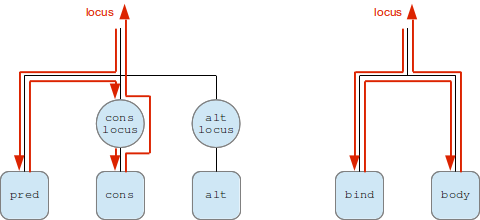
\includegraphics{images/eval_if_let.png}
\caption{On the left, the locus flow inside an evaluation of a conditional structure whom predicate has not been evaluated to \ischeme{\#f}. On the right, the locus flow inside an evaluation of a binding.}
\label{eval_if_let}
\end{figure}

\paragraph{Let evaluation} First we extract all the information contained inside the expression. Then we evaluate the binding and get back both a modified locus and a value. Now we have the binding value we can extend the environment. In case the binding is a procedure definition, we must support recursion and update the environment of the returned monomorphic procedure. The body of the let can now be evaluated with the extended environment and the modified locus:
\begin{scheme}
;; (let <param> <bind> <body>)
(define (eval-let expr env locus)
  (let* ((param      (car (cdr expr)))
         (bind       (car (cdr (cdr expr))))
         (body       (car (cdr (cdr (cdr expr)))))
         (bind-lval  (eval bind env locus))
         (bind-value (lval-value bind-lval))
         (bind-locus (lval-locus bind-lval))
         (ext-env    (dico:add env param bind-value)))
    (when (tagged-list? (car (cdr (cdr expr))) 'lambda)
      (set-monoproc-env! bind-value ext-env))
    (eval body ext-env bind-locus)))
\end{scheme}

\paragraph{Subtyping evaluation} This rule allows to instantiate polymorphic procedures. After evaluating the supposed polymorphic procedure it returns a \ischeme{poly} structure made of information contained inside the given expression:
\begin{scheme}
;; (sub <polytype> <monotype> <proc>)
(define (eval-sub expr env locus)
  (let* ((polytype (car (cdr expr)))
         (monotype (car (cdr (cdr expr))))
         (proc (car (cdr (cdr (cdr expr)))))
         (proc-lval (eval proc env locus))
         (proc-locus (lval-locus proc-lval))
         (proc-value (lval-value proc-lval)))
    (lval proc-locus (polyproc polytype monotype proc-value))))
\end{scheme}

\paragraph{Application evaluation} First the argument is evaluated then a case analysis on the procedure is performed:
\begin{scheme}
;; (<proc> <arg>)
(define (eval-app expr env locus)
  (define (apply-prim proc-value arg-value locus) ...)
  (define (apply-mono proc-value arg-value locus) ...)
  (define (apply-poly proc-value arg-value locus) ...)
  (let* ((proc       (car expr))
         (arg        (car (cdr expr)))
         (proc-lval  (eval proc env locus))
         (proc-locus (lval-locus proc-lval))
         (proc-value  (lval-value proc-lval))
         (arg-lval   (eval arg env proc-locus))
         (arg-locus  (lval-locus arg-lval))
         (arg-value  (lval-value arg-lval)))
    (cond ((procedure? proc-value) (apply-prim proc-value arg-value arg-locus))
          ((monoproc? proc-value) (apply-mono proc-value arg-value arg-locus))
          ((polyproc? proc-value) (apply-poly proc-value arg-value arg-locus))
          (else (error "cannot apply")))))
\end{scheme}
\begin{enumerate}
\item \emph{Primitive}: Primitive procedure does not modify the locus \reffig{mono_poly_prim}, we simply wrap the result of the primitive application inside a \ischeme{lval} structure:
\begin{scheme}
(define (apply-prim proc-value arg-value locus)
  (lval locus (proc-value arg-value)))
\end{scheme}
\item \emph{Monomorphic}: This application is very similar to the application of standard Scheme compound procedure \reffig{mono_poly_prim}, we only have to give the current locus to perform the body evaluation:
\begin{scheme}
(define (apply-mono proc-value arg-value locus)
  (eval (monoproc-body proc-value)
        (dico:add env (monoproc-param proc-value) (arg-value))
        locus))
\end{scheme}
\item \emph{Polymorphic}: This application actually implements the polymorphic wrapper of monomorphic procedure \reffig{mono_poly_prim}, we must enforce the locus before the monomorphic application and release it after:
\begin{scheme}
(define (apply-poly proc-value arg-value locus)
  (let* ((monoproc       (polyproc-monoproc proc-value))
         (polytype       (polyproc-polytype proc-value))
         (monotype       (polyproc-monotype proc-value))
         (enforced-locus (locus:enforce locus polytype monotype))
         (lval-mono      (apply-mono monoproc arg-value enforced-locus)))
    (lval (locus:release (lval-locus lval-mono) polytype)
          (lval-value lval-mono))))
\end{scheme}
\end{enumerate}

\begin{figure}
\centering
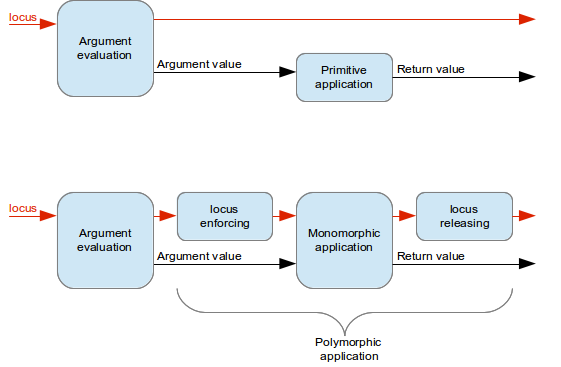
\includegraphics{images/mono_poly_prim.png}
\caption{The evolution of the locus and the value during the three different kind of applications: primitive, monomorphic and polymorphic.}
\label{mono_poly_prim}
\end{figure}

\section{Compilation $\lang\to\lang\lang$}

\emph{Objectives} The compiler $\lang\to\lang\lang$ has been developed following those two main objectives:
\begin{enumerate}
\item The type deduction inside a conditional branch should never affect the type deduction out of that branch.
\item The type generalization of a procedure should concern all the type variables introduced during the body compilation that does not affect the external type variables.
\end{enumerate}
The first objective is a translation of the iterative leitmotiv which is to avoid making restrictive assumptions during the static code analysis. The second objective maximize the constraints releasing after a polymorphic call. Lets analyze the following $\lang\lang$ pseudo code that did not generalized \ischeme{b} for the polymorphic procedure \ischeme{useless-read}:
\begin{scheme}
(define (useless-read x)
  (sub (\-/in.()->in) (()->b) read)
  x)

((sub (\-/a.a->a) (Num->Num) useless-read) 1)
((sub (\-/a.a->a) (Str->Str) useless-read) "foo")
\end{scheme}
The type of \ischeme{useless} has been inferred to \ischeme{\-/a.a->a}. As a result, the constraint on \ischeme{b} is not released after the first polymorphic call and the second input must have the same type as the first one. This is not a correct behavior for polymorphic procedures. The problem is avoided if the type of \ischeme{useless} is inferred to \ischeme{\-/a,b.a->a}. This example highlights the necessity to link all the type variables introduced inside the body of a polymorphic procedure that does not affect the external type variables.

\paragraph{Markers} The second objective could be fulfilled by storing the generated variables during the compilation. However, this solution does not scale well with the delayed compilation of conditional structure. Instead of using explicit lists we preferred to use markers to define sets of linked variables. In consequence, the polytype $\forall a_1,\ldots,a_N.\tau$ is now represented by: $\forall a.\tau$ which means that all the type variables marked with $a$ are linked. In other words, when two type variables share the same marker that means they are linked into the same polytype.

\paragraph{Interfaces}
\begin{itemize}
\item \emph{Type interface}: Beside markers this type interface implements very standard concepts concerning types:
\begin{enumerate}
\item \ischeme{(define (type:type-of constant) ...)}: implementation of $typeOf$ function.
\item \ischeme{(define (type:make-poly marker monotype) ...)}: creates a polytype from a marker and a monotype.
\item \ischeme{(define (type:poly? type) ...)}: tells if the given argument is a polytype.
\item \ischeme{(define (type:sub polytype) ...)}: returns a generic instance of the given polytype.
\item \ischeme{(define (type:make-abs arg-type res-type) ...)}: the functional type constructor: $\to$.
\item \ischeme{(define (type:abs-arg type) ...)}: returns the argument type of a function type.
\item \ischeme{(define (type:abs-res type) ...)}: returns the result type of a function type.
\item \ischeme{(define (type:make-marker!) ...)}: returns a never-used marker.
\item \ischeme{(define (type:make-var! marker) ...)}: returns a never-used type variable containing the given marker.
\end{enumerate}
\item \emph{Locus interface}:
\begin{enumerate}
\item \ischeme{(define (locus:make-empty) ...)}: returns a locus without any constraint.
\item \ischeme{(define (locus:union locus1 locus2) ...)}: classic locus unification
\item \ischeme{(define (locus:add locus type1 type2) ...)}: unification of a locus and the new constraint \ischeme{[type1 => type2]}.
\item \ischeme{(define (locus:close! locus marker) ...)}: create a closure inside the given locus for the given marker. The marker of some variable may be mutated in the process. 
$$\ischeme{[a1 => b2, b3 => String]}\xlongrightarrow{\ischeme{close! a}}\ischeme{[a1 => a2, b3 => String]}$$
\item \ischeme{(define (locus:project locus ass) ...)}: instantiate all the free variables contained in the assumptions following the given locus.
\end{enumerate}
\item \emph{Dictionary interface}: Same interface as for the environment in the $\lang\lang$ evaluator.
\end{itemize}

\paragraph{Structures} To improve readability, we dedicate a structure for the return values of the compilers:
\begin{scheme}
(struct idiom (type expr locus))
\end{scheme}

\paragraph{Overall compilation} As for the interpretation, the overall compilation start with a case analysis that dispatches the compilation to specific procedures like \ischeme{compile-const}:
\begin{scheme}
(define (compile expr ass marker)
  (cond ((tagged-list? expr 'lambda) (compile-abs expr ass marker))
        ((tagged-list? expr 'let)    (compile-let expr ass marker))
        ((tagged-list? expr 'if)     (compile-if expr ass marker))
        ((symbol? expr)              (compile-id expr ass marker))
        ((not (list? expr))          (compile-const expr ass marker))
        (else                        (compile-app expr ass marker))))
\end{scheme}

\paragraph{Constant compilation} No constraints are generated and so the empty locus is returned. The constant remains intact and its type is given by \ischeme{type:type-of} which implements the $typeOf$ function:
\begin{scheme}
;; CONST => CONST
(define (compile-const expr ass marker)
  (idiom (type:type-of expr)
         expr
         (locus:make-empty)))
\end{scheme}

\paragraph{Abstraction evaluation} We assume that the type of the argument is an arbitrary type variable which produces the assumption: \ischeme{param:arg-var}. \ischeme{ext-ass} is the union of this new assumption with the old ones. The body is then compiled with \ischeme{ext-ass} and \ischeme{marker}:
\begin{scheme}
;; (lambda <param> <body>) => (lambda <param> <compiled-body>)
(define (compile-abs expr ass marker)
  (let* ((param ((car (cdr expr))))
         (body ((car (cdr (cdr expr)))))
         (arg-var (type:make-var! marker))
         (ext-ass (dico:add ass param arg-var))
         (body-idiom (compile body ext-ass marker)))
    (idiom (type:make-abs arg-var (idiom-type body-idiom))
           (list 'lambda param (idiom-expr body-idiom))
           (idiom-locus body-idiom))))
\end{scheme}

\paragraph{Application compilation} We compile separately the procedure and the argument. The overall type is given by the return type of the procedure. The overall locus is given by the unification of the procedure locus, the argument locus and the constraint that links the expected argument with the actual argument:
\begin{scheme}
;; (<proc> <arg>) => (<compiled-proc> <compiled-arg>)
(define (compile-app expr ass marker)
  (let* ((abs (car (expr)))
         (arg (car (cdr expr)))
         (abs-idiom (compile abs ass marker))
         (arg-idiom (compile arg ass marker)))
    (idiom (type:abs-res (idiom-type abs-idiom))
           (list (idiom-expr abs-idiom) (idiom-expr arg-idiom))
           (locus:add (locus:union (idiom-locus abs-idiom) (idiom-locus arg-idiom))
                      (type:abs-arg (idiom-type abs-idiom)) (idiom-type arg-idiom)))))
\end{scheme}

\paragraph{Identifier compilation} We first lookup for type associated to the identifier inside the assumption set. Then we differentiate the case when the binding is a monotype or polytype:
\begin{scheme}
;; SYMBOL => SYMBOL
;;        => (<polytype> <monotype> SYMBOL)
(define (compile-id expr ass marker)
  (define (compile-poly-id polytype) ...)
  (define (compile-mono-id monotype) ...)
  (let ((bind (dico:lookup ass expr)))
    (if (type:poly? bind)
        (compile-poly-id bind)
        (compile-mono-id bind))))
\end{scheme}
\begin{itemize}
\item \emph{Monotype binding}: An idiom is returned containing the monotype, the symbol and an empty locus (no constraints are generated):
\begin{scheme}
(define (compile-mono-id monotype)
  (idiom monotype
         expr
         (locus:make-empty)))
\end{scheme}
\item \emph{Polytype binding}: Again, no constraints are generated ; both the polytype and a generic instance the polytype are stored inside a $sub$ expression:  
\begin{scheme}
(define (compile-poly-id polytype)
  (let ((monotype (type:sub polytype marker)))
    (idiom monotype
           (list 'sub polytype monotype expr)
           (locus:make-empty))))
\end{scheme}
\end{itemize}

\paragraph{Binding compilation} We first extract the different parts of the let expression and then perform a case analysis on whether the binding is an abstraction or not:
\begin{scheme}
;; (let <param> <bind> <body>) => (let <param> <compiled-bind> <compiled-body>)
(define (compile-let expr ass marker)
  (define (compile-let-abs param bind body) ...)
  (define (compile-let-rest param bind body) ...)
  (let ((param (car (cdr expr)))
        (bind  (car (cdr (cdr expr))))
        (body  (car (cdr (cdr (cdr expr))))))
    (if (tagged-list? bind 'lambda)
        (compile-let-abs param bind body)
        (compile-let-rest param bind body))))
\end{scheme}
\begin{enumerate}
\item \emph{Other binding}: The binding is not a procedure definition, the expression $(let\ x\ bind\ body)$ is equivalent to $((lambda\ x\ body)\ bind)$:
\begin{scheme}
(define (compile-let-rest param bind body)
  (let* ((bind-idiom (compile bind ass))
         (ext-ass (dico:add ass param (idiom-type bind-idiom)))
         (body-idiom (compile body ext-ass)))
    (idiom (idiom-type body-idiom)
           (list 'let param (idiom-expr bind-idiom) (idiom-expr body-idiom))
           (locus:union (idiom-locus bind-idiom) (idiom-locus body-idiom)))))
\end{scheme}
\item \emph{Procedure binding}: The binding is a procedure and the we must handle recursion and polymorphism.
\begin{itemize}
\item \ischeme{bind-marker}: a never-use marker to create type variables inside the binding.
\item \ischeme{bind-var}: the type the binding perceive from itself. Since the binding perceive itself as a monomorphic type, the recursion is monomorphic.
\item \ischeme{mono-ext-ass}: the assumption set inside which the binding will be compiled.
\item \ischeme{bind-idiom}: the result of the binding compilation with the extended assumptions \ischeme{mono-ext-ass} and the new marker \ischeme{bind-marker}.
\item \ischeme{bind-monotype}: the type of the binding returned by the compilation.
\item \ischeme{bind-polytype}: the generalization of \ischeme{bind-monotype}.
\item \ischeme{bind-locus}: the locus generated by the binding compilation with the additional constraint \ischeme{bind-var => bind-monotype}.
\item \ischeme{poly-ext-ass}: the assumption set inside which the body will be compiled.
\item \ischeme{body-idiom}: the result of the body compilation with the extended assumption \ischeme{poly-ext-ass} and the old marker \ischeme{marker}.
\end{itemize}
The general type of the expression is monotype returned by the body compilation. The compiled expression is: \ischeme{(let <param> <compiled-bind> <compiled-body>)}. The total locus is the union of  \ischeme{bind-locus} and the locus returned by the body compilation:
\begin{scheme}
(define (compile-let-abs param bind body)
  (let* ((bind-marker (type:make-marker!))
         (bind-var (type:make-var! bind-marker))
         (mono-ext-ass (dico:add ass param bind-var))
         (bind-idiom (compile bind mono-ext-ass bind-marker))
         (bind-monotype (idiom-type bind-idiom))
         (bind-polytype (type:make-poly marker bind-monotype))
         (bind-locus (locus:add (idiom-locus bind-idiom) bind-var bind-monotype))
         (poly-ext-ass (dico:add ass param bind-polytype))
         (body-idiom (compile body poly-ext-ass marker)))
    (locus:close! bind-locus marker)
    (idiom (idiom-type body-idiom)
           (list 'let param (idiom-expr bind-idiom) (idiom-expr body-idiom))
           (locus:union bind-locus (idiom-locus body-idiom)))))
\end{scheme}
\end{enumerate}

\paragraph{Conditional structure compilation} The compilation of conditional structure is first delayed inside a structure that contains useful information like the current marker and the current environment:
\begin{scheme}
;; (if <pred> <then> <else>)
;;   => (delay <type-var> <marker> <ass> <compiled-pred> <then> <else>)
(define (compile-if expr ass marker)
  (let* ((pred (car (cdr expr)))
         (then (car (cdr (cdr expr))))
         (else (car (cdr (cdr expr))))
         (pred-idiom (compile pred ass))
         (var (type:make-var! marker)))
    (idiom var
           (list 'delay var marker ass (idiom-expr pred-idiom) then else)
           (idiom-locus pred-idiom))))
\end{scheme}
The idea that lurks behind that delayed compilation is simple: the direct context must be completely analyzed before we can analyze each branch separately \reffig{synt_tree}. By doing this we can ensure both branch are compatible with the direct context. This would not be the case if the syntax tree was constructed purely depth first. 

\begin{figure}
\centering
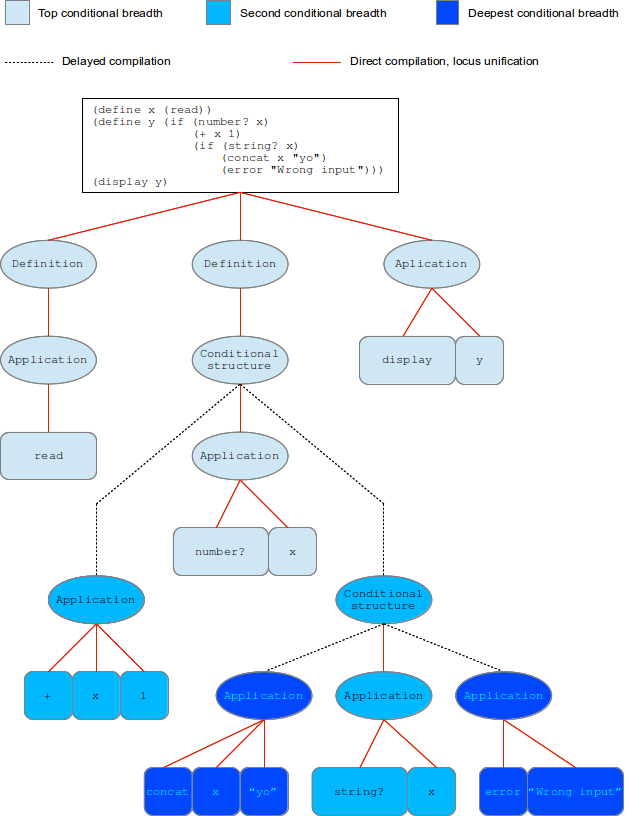
\includegraphics{images/synt_tree.png}
\caption{The syntax tree as constructed by the compiler $\lang\to\lang\lang$ for the upper program. Each color represents a different conditional breadth. The current breadth is totally compiled before jumping to deeper breadth. Inside a breadth, all the generated loci are unified.}
\label{synt_tree}
\end{figure}

\paragraph{Delay compilation} This is the actual compilation of the conditional structure. Given the locus that characterizes the direct context we search for delayed conditional structures:
\begin{scheme}
(define (finalize tree locus)
  (cond ((tagged-list? tree 'delay) (finalize-delay tree locus))
        ((list? tree) (map (lambda (tree) (finalize tree locus)) tree))
        (else tree)))
\end{scheme}
Once a delayed conditional structure has been found we first extract all the information. Then we incorporate the given locus, that represents the direct context, inside the stored assumption set. We then evaluate and finalize separately each branch:
\begin{scheme}
;; (delay <var> <marker> <ass> <compiled-pred> <then> <else>)
;; => (if <compiled-pred> <then-locus> <compiled-then> <else-locus> <compiled-else>)
(define (finalize-delay delay locus)
  (let* ((var           (car (cdr delay)))
         (marker        (car (cdr (cdr delay))))
         (ass           (car (cdr (cdr (cdr delay)))))
         (compiled-pred (car (cdr (cdr (cdr (cdr delay))))))
         (then          (car (cdr (cdr (cdr (cdr (cdr delay)))))))
         (else          (car (cdr (cdr (cdr (cdr (cdr (cdr delay))))))))
         (projected-ass (locus:project locus ass))
         (then-idiom    (compile then projected-ass marker))
         (then-locus    (locus:add (idiom-locus then-idiom) var (idiom-type then-idiom)))
         (then-expr     (finalize (idiom-expr then-idiom) then-locus))
         (else-idiom    (compile else projected-ass marker))
         (else-locus    (locus:add (idiom-locus else-idiom) var (idiom-type else-idiom)))
         (else-expr     (finalize (idiom-expr else-idiom) else-locus)))
    (list 'if compiled-pred then-locus then-expr else-locus else-expr)))
\end{scheme}

\section{Conclusion}

We opened this chapter with some very common concepts in type theory. We then introduced a classic language to deal with type system ; we called it $\lang$. We also demonstrated that $\lang$, beside assignments, has the same expressiveness as LScheme. Afterwards, an Hindley-Milner type system was introduced as a strong theoretical base for iterative type system. The next section exposed the $\lang$ type system as a slightly modified Hindley-Milner type system. Then the $\lang\lang$ language, which is the annotated version of $\lang$, and its type system were presented. The following section defined some operations on loci. Finally we had everything in hands to expose the compilation $\lang\to\lang\lang$ and the evaluation of $\lang\lang$ expressions.

%%%%%%%%%%%%%%%%%%%%%%%%%%%%%%%%%%%%%%%%
%%%%%%%%%%%%%%%%%%%%%%%%%%%%%%%%%%%%%%%%
%%%%%%%%%%%%%%%%%%%%%%%%%%%%%%%%%%%%%%%%
%%%%%%%%%%%%%%%%%%%%%%%%%%%%%%%%%%%%%%%%
\chapter{Related Works\label{ch_related}}
%%%%%%%%%%%%%%%%%%%%%%%%%%%%%%%%%%%%%%%%
%%%%%%%%%%%%%%%%%%%%%%%%%%%%%%%%%%%%%%%%
%%%%%%%%%%%%%%%%%%%%%%%%%%%%%%%%%%%%%%%%
%%%%%%%%%%%%%%%%%%%%%%%%%%%%%%%%%%%%%%%%

In this chapter, we will introduce soft and gradual typing, two newly created typings that attempt to mix static and dynamic typings. We then compare iterative typing with those researches.

\section{Soft Typing}

\paragraph{Introduction} This section is strongly inspired from \cite{soft1} and \cite{soft3}. Soft typing is an attempt to increase the static safety of dynamic programs. Soft typing first performs a static type inference. When an primitive application can not be proven safe, a runtime check is inserted. Soft typing can be seen as a dynamic typing that statically performs as many type checks as possible.

\paragraph{Soft type system} Soft typing uses an elaborate type system based on union types, a typing discipline that can express that a variable can have multiple types at the execution. For instance $Number|Null$ is the type of an expression that may either be of type number or be the null constant. This expressive power allows soft typing to handle many common Scheme patterns. The specificity of the soft type system is encapsulate by two rules about applications \reffig{soft_ts}. The first application rule, labeled APP, concerns the applications that have been proven safe. The second application rule, labeled CHECK-APP, concerns unsafe applications that must be checked at runtime. When CHECK-APP is not used at all, the program is statically type safe.

\begin{table}
\begin{tabular}{cc}
$$
\LeftLabel{[APP]}
\ax{A\vdash e_1:(\tau_2\to\tau_1)\cup\varphi}
\ax{A\vdash e_2:\tau_2}
\bic{A\vdash (app\ e_1\ e_2):\tau_1}
\drule
$$
&
$$
\LeftLabel{[CHECK-APP]}
\ax{A\vdash e_1:(\tau_2\to\tau_1)\cup\tau_3}
\ax{A\vdash e_2:\tau_2}
\bic{A\vdash (check-app\ e_1\ e_2):\tau_1}
\drule
$$
\end{tabular}
\caption{The two application rules of the soft type system. The left one concerns safe applications, the right one concerns unsafe applications that must be checked at the execution.}
\label{soft_ts}
\end{table}

\paragraph{Example} Here is the the \ischeme{flatten} function, it takes a tree and return list of all the leaves:
\begin{scheme}
(define (flatten xs)
  (cond ((null? xs) null)
        ((pair? xs) (append (flatten (car xs)) (flatten (cdr xs))))
        (else (list xs))))
(flatten '(1 (2 3) 4))
\end{scheme}
\begin{shell}
'(1 2 3 4)
\end{shell}
The authors of \cite{soft3} present the above program as a success story because it is statically type safe for soft typing. In comparison, iterative typing cannot support such program because it uses heterogeneous lists.

\paragraph{Criticisms} Although able to remove many runtime checks from Gabriel benchmarks, which standard benchmarks to validate a lisp implementation, soft typing suffer from severe criticisms:
\begin{enumerate}
\item \emph{Unnecessary runtime checks}: The proposed type system does not succeed to infer the precise type of some much used procedures like \ischeme{map}. As a result every \ischeme{map} call will generate runtime checks even those who are trivially safe like \ischeme{(map (lambda (x) (+ x 1)) (list 1 2 3))}.
\item \emph{Expressiveness restriction}: Though very permissive, the soft type system still rejects some well typed programs. In particular, the \ischeme{if} expressions are statically analyzed ; the two branches must be type compatible.
\end{enumerate}

\section{Gradual Typing}

\paragraph{Introduction} This section is strongly inspired from\cite{grad3}. Gradual typing is meant to perform a smooth transition from scripts to static programs. So, as soft typing, gradual typing also combines static and dynamic typing. But their approach are radically different. When soft typing provides unsafe primitive application, gradual typing provides a so called dynamic type that always pass static checks. This type is annotated $?$ and represents values that can be anything at the execution. Variables annotated with such tag will generate casts and as many runtime checks.

\paragraph{Consistency relation} The consistency relation, notated $\sim$, replaces the subtyping relation usually used in type systems. Saying that a type must never fail a static checks is equivalent to say it must be compatible with any other type. This justifies the following axioms:
$$\begin{array}{ccccccc}
?\sim\tau
&&
\tau\sim ?
&&
\tau\sim\tau
&&
\ax{\tau_1\sim\tau_2}
\ax{\tau_1'\sim\tau_2'}
\bic{\tau_1\to\tau_1'\sim\tau_2\to\tau_2'}
\drule\\
\end{array}$$

\paragraph{Gradual type system} Gradual typing is based on the simply typed lambda calculus \cite{typedlambda}. But type annotations are not mandatory ; the dynamic type is inserted every where annotations are missing. In other word: "$(\lambda\ x\ e)$" is a syntactic sugar for "$(\lambda \ (x:?) e$". As explain before, the gradual type system use the consistency relation instead of the classic subtype relation. In \reffig{grad_ts} are exposed the most representative rules of gradual typing.

\begin{figure}
\centering
$$\begin{array}{cc}
\ax{A\vdash e_1:?}
\ax{A\vdash e_2:\tau_2}
\bic{A\vdash (e_1\ e_2):?}
\drule
&
\ax{A\vdash e_1:\tau\to\tau'}
\ax{A\vdash e_2:\tau_2}
\ax{A\vdash\tau\sim\tau_2}
\tric{A\vdash (e_1\ e_2):\tau}
\drule
\end{array}$$
\caption{Two gradual rules about applications that show how dynamic type is handled.}
\label{grad_ts}
\end{figure}

\paragraph{Cast insertion} Everywhere applications statically involve the dynamic type, casts are inserted. For instance the wrapping of the increment procedure:
$$(\lambda\ (x)\ (increment\ x))\xlongrightarrow{compilation}(\lambda\ (x:?)\ (increment\ \langle Number\rangle x))$$
The annotation $(x:Number)$ would have prevented the insertion of the cast $\langle Number\rangle x$.

\paragraph{Compilation} Gradual typing provide an algorithm that automatically insert type annotations so the programmer does not have to manually sort the variables that should be statically checked and the variable that should be dynamically checked.

\paragraph{Result}
\begin{enumerate}
\item The execution of compiled program (with inserted casts) can not lead to an uncaught type error.
\item If a program free of the dynamic type is entirely statically checked. In other words, if such program pass the static then it is type safe.
\item After a simple wrapping manipulation, all the programs are accepted. The gradual typing can be as expressive as a pure dynamically typed language based on the lambda calculus.
\end{enumerate}

\section{Comparison with iterative typing}

\paragraph{Runtime checks} Lets consider a simple Scheme code, that asks the user a radius the compute the circumference and the surface of the associated circle:
\begin{scheme}
(define radius        (read))
(define pi            3.14)
(define circumference (* 2 (* pi radius)))
(define surface       (* pi (* radius radius)))
\end{scheme}
Each exposed typing techniques insert runtime checks in its own way:
\begin{enumerate}
\item \emph{Soft typing compilation} The return type of \ischeme{read} is an union of string, number, etc. Therefor any primitive call that involves \ischeme{radius} must be checked at runtime:
\begin{scheme}
(define radius        (read))
(define pi            3.14)
(define circumference (* 2 (CHECK-MULT pi radius)))
(define surface       (pi (CHECK-MULT radius radius)))
\end{scheme}
The uncertainty on \ischeme{radius} led to two unsafe primitive applications. If the user entered a wrong input, the error is detected at the \ischeme{circumference} definition.
\item \emph{Gradual typing compilation} The return type of \ischeme{read} is the dynamic type. Therefor any applications, that involves \ischeme{radius} and requires non dynamic types as argument, generates runtime cast on \ischeme{radius}:
\begin{scheme}
(define radius:?             (read))
(define pi:Number            3.14)
(define circumference:Number (* 2 (pi <Number>radius)))
(define surface:Number       (* pi (<Number>radius <Number>radius)))
\end{scheme}
The checks that ensure \ischeme{radius} is a number is performed thrice. If the user did not enter a number, the error is detected at the first use, at the \ischeme{circumference} definition.
\item \emph{Iterative typing compilation} Iterative typing detect \ischeme{read} should return a number, only one check is required at the \ischeme{read} call:
\begin{scheme}
(define radius        ((in => Number) read))
(define pi            3.14)
(define circumference (* 2 (* pi radius)))
(define surface       (* pi (* radius radius)))
\end{scheme}
The type of \ischeme{radius} is only checked once right at the read primitive call. 
\end{enumerate}
As we can see, Iterative typing have the ability to summarize and move upward the checks inserted by soft and gradual typing. As a result, less runtime checks are performed and they are performed earlier on more relevant places.

\paragraph{Expressiveness} The cost of having less runtime checks on better places is a restricted expressiveness. Here are examples of valid Scheme programs that are not currently accepted by iterative typing:
\begin{itemize}
\item \emph{Polymorphism}: polymorphic use of argument inside a procedure:
\begin{scheme}
(define (use-poly f)
  (f 1)
  (f "foo"))
(use-poly (lambda (x) x))
\end{scheme}
\begin{shell}
"foo"
\end{shell}
\item \emph{Heterogeneous lists}: manipulation of heterogeneous lists:
\begin{scheme}
(define (use-hetero xs)
  (cond ((null? xs) null)
        ((string? (car xs)) (cons (concat "yo " (car xs)) (use-hetero (cdr xs))))
        ((number? (car xs)) (cons (* 2 (car xs))) (use-hetero (cdr xs)))
        (else (error "non handeled type"))))
\end{scheme}
\begin{shell}
'("yo foo" 2 "yo bar" 4 6)
\end{shell}
\end{itemize}

\paragraph{Type tag} Gradual and soft typing can both be seen as dynamic typing which perform as many checks as possible during a static code analysis. Iterative typing goes the other way around, it is a static typing that delays as few checks as possible at runtime. Soft and gradual typings both use type tags to perform runtime checks during the interpretation while the iterative interpreter don't need them to ensure safety. The only places where the schemes primitives like \ischeme{number?} and \ischeme{string?} occur are inside the implementation of LLScheme primitives. For instance the LLScheme primitive \ischeme{string?} calls the Scheme primitive \ischeme{string?}.

\section{Conclusion}

Soft and gradual typings both propose an interesting mix between static and dynamic typings. Iterative typing succeed to summarize soft and gradual runtime checks and move them on an upper level. The cost having a earlier error detection is a diminished expressiveness.

%%%%%%%%%%%%%%%%%%%%%%%%%%%%%%%%%%%%%%%%
%%%%%%%%%%%%%%%%%%%%%%%%%%%%%%%%%%%%%%%%
%%%%%%%%%%%%%%%%%%%%%%%%%%%%%%%%%%%%%%%%
%%%%%%%%%%%%%%%%%%%%%%%%%%%%%%%%%%%%%%%%
\chapter{Future Works\label{ch_future}}
%%%%%%%%%%%%%%%%%%%%%%%%%%%%%%%%%%%%%%%%
%%%%%%%%%%%%%%%%%%%%%%%%%%%%%%%%%%%%%%%%
%%%%%%%%%%%%%%%%%%%%%%%%%%%%%%%%%%%%%%%%
%%%%%%%%%%%%%%%%%%%%%%%%%%%%%%%%%%%%%%%%

\section{Overloading}

This section is about how simulate overloading behavior with the \ischeme{if-viable} iterative special form. A lot of investigations are needed to understand all the consequences of \ischeme{if-viable} special form. One consequence that makes the \ischeme{if-viable} very dangerous is that it introduces a new semantic that does not exist in Scheme, so this extended iterative typing is not only about detecting errors earlier but also express new concepts.

\paragraph{Overloading} Overloading is a very important feature of most modern programming languages that allows creating several methods with the same name which differ from each other in the type of inputs and the output of the function. That is, the concrete body is defined by the calling context at compile time. In the following Java program, the rectangle constructor is overloaded which allows creating rectangles from two points or with two integers:
\begin{java}
class Rectangle () {
	private Point a;
	private Point b;
	// Construct a rectangle defined by the given points.
	Rectangle(Point a, Point b) {
		this.a = a;
		this.b = b;
	}
	// Construct a rectangle with one of its vertices located on the origin.
	Rectangle(int width, int height) {
		a = new Point(0,0);
		b = new Point(width, height);
	}
}
\end{java}
When overloading on inputs is present on most mainstream languages, output overloading is less common because it produces ambiguities. One notable exception being Haskell that does support output overloading trough type classes\cite{haskell}. Lets suppose Java supports output overloading and we want to simplify the use of the \ijava{Random} class, we would then write the following code:
\begin{java}
int random() {
	(new Random()).nextInt();
}

float random() {
	(new Random()).nextFloat();
}

long random() {
	(new Random()).nextLong();
}

void test() {
	System.out.println(random()); // which random body???
}
\end{java}
Indeed, the use of \ijava{random} inside \ijava{test} is ambiguous and that is why output overloading, although handy, is often avoided.

\paragraph{Viability tests} The iterative \ischeme{if-viable} must not be confused with the standard \icode{try} constructions. The \ischeme{try} construction performs code until an exceptions is raised and call the exception handler. On the other hand, iterative typing does not execute any code, it just tests if the first branch is viable inside the current context. In other words, \ischeme{if-viable} is semantically equivalent to an iterative \ischeme{if} containing a test about the viability of the first branch as a predicate:
\begin{scheme}
(if-viable <attempt>
           <alternative>)
\end{scheme}
Is equivalent to:
\begin{scheme}
(if <attempt viable?>
    <attempt>
    <alternative>)
\end{scheme}

\paragraph{Iterative typing} With early error detection, iterative typing is able to grab some information about the calling context. This is achieved be proposing several bodies inside a \ischeme{try} structure, iterative typing will loop through those proposition until it find one that is viable:
\begin{scheme}
(define (<name> <args>)
  (if-viable <body1>
             ...
             <bodyN>))
\end{scheme}
If iterative typing reaches the last proposition, it will be executed even if not viable. Notice that this naturally resolves the ambiguities usually introduced by output overloading.

\paragraph{Knowing your arguments} For input overloading, the iterative \ischeme{if-viable} structure is close to regular \icode{try} structures. That is, the viability of the proposition itself is tested not its future consequences:
\begin{scheme}
(define pimp-my-arg (lambda (x)
                      (if-viable (concat x "bunta")
                                 (+ x 3))))
(pimp-my-arg 1)
(pimp-my-arg "gama ")
\end{scheme}
\begin{shell}
4
"gama bunta"
\end{shell}

\paragraph{Knowing your result} For output overloading, the iterative \ischeme{if-viable} has a different behavior than regular \icode{try} structures. That is, the future consequences of the proposition is tested:
\begin{scheme}
(define pimp-my-result (lambda ()
                (if-viable "party"
                           1)))
(+ (pimp-my-result) 2)
(concat (pimp-my-result) " rocking")
\end{scheme}
\begin{shell}
3
"party rocking"
\end{shell}

\section{Polymorphic recursion}

\paragraph{Monomorphic recursion} For now, iterative typing implements monomorphic recursion. Inside a monomorphic recursive computation, types are not allowed to change: each recursive call accepts the same argument and result type. The factorial mathematic function is a typical example of monomorphic recursion ; the recursive procedure always takes a number as argument and return a number as well:
\begin{scheme}
;; fac :: Number -> Number
(define (fac n)
  (if (= n 0)
      1                     ; return a number
      (* n (fac (- n 1))))) ; return a number
\end{scheme}
It is also possible to produce polymorphic procedure that use monomorphic recursion. Below we propose a Scheme program that defines a procedure which creates a list containing \ischeme{n} times the data \ischeme{x}:
\begin{scheme}
;; several :: \-/ a . a Number -> [a]
(define (several x n)
  (if (= n 0)
      null                           ; return a polymorphic constant
                                     ; that is interpreted as [a]
      (cons x (several x (- n 1))))) ; return [a]
\end{scheme}
This procedure is polymorphic because it accepts the call \ischeme{(several 0 10)} but also the call \ischeme{(several "foo" 10)}. Nevertheless, the type variable $a$ is defined only once at the top level call and never change during the recursive computation. If \ischeme{(several "foo" 3)} is invoked, the procedure \ischeme{several} will always have the type $String ~ Number \to [String]$ \reffig{rec_stack}.

\begin{figure}
\centering
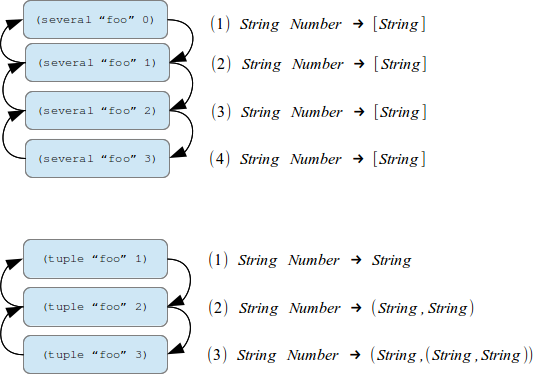
\includegraphics{images/rec_stack.png}
\caption{In a monomorphic recursion, the recursive call are always perform on the same type. In a polymorphic recursion the type may vary from one recursive call to an other.}
\label{rec_stack}
\end{figure}

\paragraph{Polymorphic recursion} On the opposite way, polymorphic recursion does allow types to change inside the recursive computation. Generally, type inference for polymorphic recursion is undecidable\cite{poly_rec}. So it is not possible to statically decide whether a polymorphic recursion is type safe or not. Below, we define the \ischeme{tuple} procedure which is somehow similar to the \ischeme{several} procedure but create a tuple instead of a list:
\begin{scheme}
;; tuple :: \-/ a . a Number -> ???
(define (tuple x n)
  (if (= n 1)
      x                            ; return a
      (pair x (tuple x (- n 1))))) ; return (a,???)
\end{scheme}
Through this polymorphic recursion a nested pair is created. To known the nesting depth and the precise type return by a \ischeme{tuple} call, we actually need to execute the code. As Scheme is Turing complete this execution may never return, as is the case for the call \ischeme{(tuple "foo" 0)}.

\paragraph{Heterogeneous list} We can interpret heterogeneous lists as nested pairs that end with the \ischeme{null} value. Below we give a small Scheme program that manipulate heterogeneous lists that way:
\begin{scheme}
;; evil-list :: \-/ a . Number -> a
(define (evil-list n)
  (cond ((<= n 0) null)
        ((prime? n) (cons "prime" (evil-list (- n 1))))
        (else (cons n (evil-list (- n 1))))))

;; evil-use :: \-/ a . a -> String
(define (evil-use xs)
  (display "\n")
  (cond ((null? xs) (display "TOUCH DOWN!!!"))
        ((prime? (length xs)) (begin (display (string-append (car xs) " length"))
                                     (evil-use (cdr xs))))
        (else (begin (display (* 2 (car xs)))
                     (evil-use (cdr xs)))))
  "end")

(evil-use (evil-list 6))
\end{scheme}
\begin{shell}
12
prime length
8
prime length
prime length
prime length
TOUCH DOWN !!!
\end{shell}
For instance the call \ischeme{(evil-list 4)} return a value of type \ischeme{(Number,(String,(String,(String,Null))))} which is very hard to compute statically. By staying at the first depth level of the polymorphic recursion iterative typing can deduce useful information without executing the code. Below we present the compilation into LScheme of the above program ; as we can see all the informations are present to perform a recursive type deduction at runtime:
\begin{scheme}
;; evil-list :: \-/ a . Number -> a
(define (evil-list n)
  (cond ([a => NULL] (<= n 0) null)
        ([a => (String,b)] (prime? n)
                           (cons "prime" ((sub [b => <next-a>] evil-list) (- n 1))))
        ([a => (Number,b)] else
                           (cons n ((sub [b => <next-a>] evil-list) (- n 1))))))

;; evil-use :: \-/ a . a -> String
(define (evil-use xs)
  (display "\n")
  (cond ([a => Void] (null? xs) (display "TOUCH DOWN!!!"))
        ([a => (String,b)] (prime? (length xs))
                           (begin (display (concat "yo " (car xs)))
                             ((sub [b => <next-a>] evil-use) (cdr xs))))
        ([a => (Number,b)] else
                           (begin (display (+ 1 (car xs)))
                           ((sub [b => <next-a>] evil-use) (cdr xs)))))
  "end")

((sub [a => c] evil-use) ((sub [a => c] evil-list) 4))
\end{scheme}

\paragraph{Recursive type serialization} Many types are naturally recursive. For instance the elements of a list can themselves be lists. In fact every generic types like list $[a]$, pairs $(a,b)$, function $a\to b$ etc are recursive in the sens they can include each other without theoretical depth limitation. The deserialization of such type have not been exposed in \refsec{sec_deser} because it require a recursive polymorphic parser which iterative typing does not currently support. Lets say we use a XML format that serializes the value \ischeme{(("abc",123),"ABC")} into:
\begin{xml}
<pair>
	<fst>
		<pair>
			<fst>
				<string>abc</string>
			</fst>
			<scd>
				<number>123</number>
			</scd>
		</pair>
	</fst>
	<scd>
		<string>ABC</string>
	</scd>
<pair>
\end{xml}
The LScheme recursive polymorphic parser would be:
\begin{scheme}
;; rec-read :: \-/ a . String -> a 
(define (rec-read input)
  (define (type (get-top-level-tag input)))
  (cond ([a => (b,c)] (equal? type "pair") (cons ((sub [b => <next-a>] rec-read)
                                                   (get "fst" input))
                                                 ((sub [c => <next-a>] rec-read)
                                                   (get "scd" input))))
        ([a => String] (equal? type "string" (get "string" input)))
        ([a => Number] (equal? type "number") (string->number (get "number" input)))
        (else (error "unknwon type"))))
\end{scheme}
As usual, LScheme polymorphic call carries the contextual type information:
\begin{scheme}
(define x ({String -> ((a,Number),b)} rec-read xml-string))
(+ 1 (cdr (car x)))
\end{scheme}
Those information will make the application crash as soon a type mismatch is detected during the recursive parsing.

\paragraph{Iterative monomorphic recursion} Because even types that do not affect the outside world are fixed as well, iterative monomorphic recursion produces undesirable constraints. Lets consider the following code that defines the factorial function with an input request at each call:
\begin{scheme}
(define (input-fac n)
  (read)
  (if (= n 0)
      1
      (* n (fac (- n 1)))))
(input-fac 6)
\end{scheme}
The return type of \ischeme{read} can only be set once. Which is very disturbing since this input does not affect the execution at all.
\begin{enumerate}
\item The user has first entered a boolean, he must continue to enter booleans to avoid dummy unification failure:
\begin{shell}
>> #t
>> #f
>> 3
Unification failed on [Boolean => Number]
\end{shell}
\item The user has first entered a string, he must continue to enter strings to avoid dummy unification failure:
\begin{shell}
>> "iter 1"
>> "iter 2"
>> "iter 3"
>> "iter 4"
6
\end{shell}
\end{enumerate}

\paragraph{Iterative polymorphic recursion} Iterative typing is well suited to support polymorphic recursion since it considers conditional branch as dynamic event which return a type variable. Therefore the code analysis stops at the recursion top level, and code execution is not required for type inference. At the execution, the locus would store information to deduce the precise type returned by the polymorphic recursion will return. Nevertheless implementation of polymorphic recursion poses a technical challenge and so far, two approaches have been investigated:
\begin{enumerate}
\item \emph{Modification of the locus structure}: for now, loci are just unordered sets of type constraint ; mirroring the recursion stack could be a solution.
\item \emph{Put version on type variables}: by introducing a version system for type variable, we could differentiate the type variables located on the same place but inside a different recursive call.
\end{enumerate}

\section{Refinement of type deduction}

\paragraph{Introduction} For now, dynamic events totally encapsulate type constraints when some deduction could be applied outside the event. Effectively there are many scenarios where some constraints of two conditional branches can be merged and moved on a upper level. Below we give two examples that show the current limit of iterative type inference:
\begin{enumerate}
\item \emph{Output deduction}: the type of conditional structure is always inferred to a type variable. Below we expose a conditional structure that always returns a string, particularity that iterative typing does not exploit for the moment:
\begin{scheme}
(define (output-gross)
  (if <pred>
      "foo"
      "bar"))
(+ (output-gross) 1)
\end{scheme}
The type of \ischeme{output-gross} is currently inferred to $\forall a . () \to a$ when $()\to String$ would have been more accurate. Such vagueness causes iterative typing to miss a static error at \ischeme{(+ (output-gross) 1}.
\item \emph{Input deduction}: type constraints generated inside a conditional branch stay inside that branch. Below we expose a conditional structure that always threat \ischeme{x} as a number:
\begin{scheme}
(define (input-gross x)
  (if <pred>
      (+ x 1)
      (+ x 2))
  "end")
(input-gross "foo")
\end{scheme}
The type of \ischeme{input-gross} is currently inferred to $\forall a . a \to String$ when $Number \to String$ would have been more accurate. Such vagueness causes iterative typing to miss a static error at \ischeme{(input-gross "foo")}.
\end{enumerate}

\paragraph{Compromise} As more and more information are exploited, the complexity of the algorithm increase. In general, a compromise has to be done between accuracy and computation cost \reffig{info_comp}. For now, iterative typing only guarantees the branches of a computation structure are all viable inside the direct context.

\begin{figure}
\centering
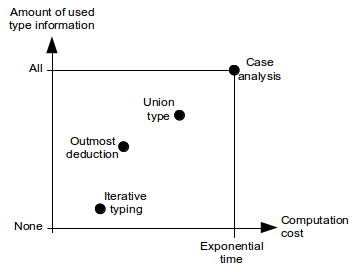
\includegraphics{images/info_comp.png}
\caption{A compromise must be done between type information given by conditional structures and computation cost. Iterative typing propose very few guarantees. Outmost deduction is a must have as it does not complicate the execution algorithm. Union typing \cite{soft3} could have a great potential but we did not investigated viability of such refinement. A complete case analysis is not practically feasible as its computation time grows exponentially with the amount of conditional structures.}
\label{info_comp}
\end{figure}

\paragraph{Outmost deduction} Without changing the type system we could detect when types share a common outmost part. Lets consider the following Scheme code and its iterative type deduction:
\begin{scheme}
;; concat-all :: [String] -> String
(define (concat-all xs)
  (if (null? xs)
      ""
      (string-append (car xs) (concat-all (cdr xs)))))

;; add-all :: [Number] -> Number
(define (add-all xs)
  (if (null? xs)
      0
      (+ (car xs) (add-all (cdr xs)))))

;; yo :: \-/ a . a -> [String]
(define (yo x)
  (if <pred>
      (concat-all x)
      (add-all x)
   "end"))
\end{scheme}
The type of \ischeme{yo} has been inferred to $\forall a . a \to String$ when $\forall a . [a] \to String$ would have been more accurate. Indeed in any case, \ischeme{x} is used as a list and a call like \ischeme{(yo #t)} would have no chance to succeed. This type errors would have been detected by a more precise type deduction. As outmost deduction would not affect the type system, only the compilation algorithm would be complicated by such improvement which makes us believe outmost deduction is a must have on iterative typing.

\paragraph{Union typing} As exposed below, union type could describes very well the semantic of dynamic conditional structures even if some static errors remain uncaught:.
\begin{enumerate}
\item \emph{Mono-union}: When only one type is affected by the conditional structure, union type is a great success:
\begin{scheme}
(define (yo)
  (if <pred>
      "foo"
      1))
(+ (yo) 1)      ; accepted
(concat (yo) 2) ; accepted
(and (yo) #f)   ; rejected
\end{scheme}
Iterative-union typing would infer the type of \ischeme{yo} to $() \to String|Number$ and so static errors like \ischeme{(and (yo) #f)} would be detected.
\item \emph{Poly-union}: when multiple types are affected through the conditional structure, some static errors are not detected:
\begin{scheme}
(define (evil x y)
  (if <pred>
      (begin (+ x 1)
             (concat y "bar"))
      (begin (+ y 1)
             (concat x "bar")))
  #t)
;; All calls are accepted
(evil 1 2)         ; static error
(evil "foo" "bar") ; static error
(evil 1 "bar")
(evil "foo" 2)
\end{scheme}
Iterative-union typing would infer the type of \ischeme{evil} to: $(String|Number,String|Number)\to Boolean$ when argument types cannot actually be the same ; calls like \ischeme{(evil 1 2)} would be erroneously accepted.
\end{enumerate}
Union typing could significantly complicate the algorithm at the execution. The viability of such improvement needs further investigations.

\paragraph{Case analysis} As presented in \refch{ch_approach}, we could detect all static type errors by performing a complete case analysis. Such an algorithm is easy to implement through a recursive procedure that calls itself twice each time a conditional structure is encountered. That way, we could investigate all possible execution traces. Nevertheless the computation time of such an algorithm grows exponentially with the amount of conditional structure which is not practically acceptable. Furthermore, in case of polymorphic recursion, such computation never ends.

\paragraph{Predicative information} So far we only discussed how informations contained in conditional branches can filter to external type deductions. But predicates give type information as well. For instance the following procedure is obviously free of type error:
\begin{scheme}
(define (guarded-operation x)
  (cond ((number? x) (+ x 1))
        ((string? x) (concat "yo" x))
        (else "errhh, dunno what to do...")))
\end{scheme}
For now, iterative does not use guard at all and some checks are redundant:
\begin{scheme}
;; guarded-operation :: \-/ a,b . a -> b
(define (guarded-operation x)
  (cond ([a => Number, b => Number] (number? x) (+ x 1))
        ([a => String, b => String] (string? x) (concat "yo" x))
        ([b => String]              else        "errhh, dunno what to do...")))
\end{scheme}
For instance, the guard \ischeme{a => Number} of the first branch is useless since that branch can only be executed if \ischeme{x} is effectively a $Number$.

%%%%%%%%%%%%%%%%%%%%%%%%%%%%%%%%%%%%%%%%
%%%%%%%%%%%%%%%%%%%%%%%%%%%%%%%%%%%%%%%%
%%%%%%%%%%%%%%%%%%%%%%%%%%%%%%%%%%%%%%%%
%%%%%%%%%%%%%%%%%%%%%%%%%%%%%%%%%%%%%%%%
\chapter{Conclusion\label{ch_concl}}
%%%%%%%%%%%%%%%%%%%%%%%%%%%%%%%%%%%%%%%%
%%%%%%%%%%%%%%%%%%%%%%%%%%%%%%%%%%%%%%%%
%%%%%%%%%%%%%%%%%%%%%%%%%%%%%%%%%%%%%%%%
%%%%%%%%%%%%%%%%%%%%%%%%%%%%%%%%%%%%%%%%

\section{Summary}

\paragraph{Context} Traditionally, languages are separated in two classes. The first class is called "dynamically typed languages". Usually those languages are very expressive but they detect errors as they happen. Scheme and JavaScript are both dynamically typed. The second class is called "statically typed languages" ; Java belongs to that class. Programs in those languages are statically analyzed which allows detecting many errors early on. Nevertheless their expressiveness is restricted and they can not denote concepts like heterogeneous lists. It is agreed that dynamic typing is handy to quickly develop prototypes while statically typed languages are well suited to develop large and robust applications. In this thesis, we developed a typing technique called iterative typing that aims to combine the best of those two worlds. In other words, iterative typing is meant to provide high expressiveness and still be able to detect errors early on.

\paragraph{Implication} On a very atomic language, earliest error detection could be obtained by performing a case analysis on dynamic events. This analysis would allow to detect errors as soon as possible when the current succession of dynamic events will, in any case, lead to an error later on. Nevertheless such algorithm is not compatible with recursion and grows exponentially with the number of dynamic events which is not theoretically and practically acceptable. Iterative typing tries to approach the case analysis behavior by dropping constraints wherever dynamic events occur. The input language is called LScheme and is very close to Scheme ; the output language is called LLScheme which is the annotated version of LScheme. As the execution goes on, dynamic uncertainties are resolved and new constraints are generated. Iterative typing carries around all the previously generated constraints and verifies the type compatibility at each new constraint generation.

\paragraph{Validation} As validation we present in this thesis three case studies of practical interest.

The most direct application of iterative typing is deserialization, that is the use of a byte sequence to instantiate a data structure whose type depends on the byte sequence value. Iterative typing allows to detect a type mismatch right inside the reading procedure. Statically typed languages can detect errors that but require heavy use of type systems. On the other hand, iterative typing completely masks the type complexity involved in the pattern.

Iterative typing can also be used to propose an alternative of the common exception handling. In the presented alternative, the exception thrower knows whether throwing an exception will cause the application to stop or if the exception will be properly handled. On the first case, the exception thrower may decide it is preferable to return an usable result instead of stopping the whole application.

The last case study is a discussion about the interaction of iterative typing and side effects. On many cases, stopping the application when iterative typing predicts an error is just fine. But, sometimes it is preferable to perform side effects until normal Scheme applications would raise an error. This justifies the unsafe execution feature that allows the programmer to shut down iterative predictions for a while.

\paragraph{Theory} A new language $\lang$ was introduced as a representation of an atomic subset of LScheme. To keep the theoretical part of this thesis as simple as possible many features were bypassed in that part. In particular, the discussed atomic subset of LScheme is free of assignments. Even simplified, LScheme is still not well suited to be described in type systems. In consequence, two new languages: $\lang$ and $\lang\lang$ were developed to mirror LScheme and LLScheme. This approach is validated by exhibiting the syntactical transformations that allows to compile LScheme to $\lang$. The theoretical presentation of iterative typing is articulated around three points. First, type systems for $\lang$ and $\lang\lang$ are both exposed and justified. Then we present a Scheme interpreter of $\lang\lang$. Finally we present a Scheme compiler from $\lang$ to $\lang\lang$ which is based on Hindley-Milner type inference\cite{hm1}.

\paragraph{Related work} Blurring the line between dynamic typing and static typing is not a recent topic. Many investigations have been performed in that sense which has led to the appearance of soft typing and gradual typing. Soft typing allows to specify whether an application should be checked during static code analysis or during the execution\cite{soft1}. Gradual typing allows to define dynamic variables that always pass static type checks but require further checks at runtime\cite{grad3}. We can say that those typings are dynamic typings that are partially statically type checked, while iterative typing is a static typing that is partially dynamically type checked. In other words, gradual and soft typing start with the status of dynamic typing and move as many type checks as possible to static code analysis. When iterative typing starts with the status of static typing and delays as little type checks as possible for the execution.

\section{Contributions} 

In this thesis, we developed a new typing technique called iterative typing. Iterative typing can be seen as a static typing that delays as little type checks as possible to the execution. This approach is new, usually the efforts made to combine static and dynamic advantages go the other way around: it is about dynamic typing that performs as many checks as possible during an additional static code analysis phase. As an illustration of that difference, soft and gradual typing explicitly use type tags to ensure safety while iterative typing does not. To apply our typing, we created two new languages called LScheme which is very close to Scheme and LLScheme which is the annotated version of LScheme. We also implemented in Scheme a compiler from LScheme to LLScheme and an interpreter of LLScheme. Iterative typing does not accept as many programs as most dynamically typed languages but it is still able to implement very dynamic patterns as exhibited in \refch{ch_eval}. The main advantage of iterative typing is the early error detection ; as shown in \refch{ch_approach} iterative typing is not remote from earliest error detection.

\section{Future work}

\paragraph{Viability testing} The \ischeme{if-viable} LScheme special form is very powerful and allows the programmer to have an insight inside iterative predictions. \ischeme{(if-viable <prop> <alt>)} can be understood as: if the execution of \ischeme{<prop>} will not produce type errors then execute \ischeme{<prop>} otherwise execute \ischeme{<alt>}. For instance, this special form can be used to simulate overloading on both inputs and output types. Nevertheless, this feature is highly experimental and increases the Scheme semantic. So far, no investigations have been performed to evaluated the consequences of such feature. 

\paragraph{Polymorphic recursion} We argue that it is possible to support polymorphic recursion inside an iterative framework. This would greatly increase the expressive power of iterative typing. For instance heterogeneous lists could be simulated by tuples manipulated by polymorphically recursive functions. Polymorphic reading procedures would allow to instantiate value of nested types like $\left[(String,[Number])\right]$ and would be a great application for iterative typing as well. The expected nested type would be deconstructed at each polymorphic recursive call and type errors would be detected at the earliest possible moment, even before the whole type would be known.

\paragraph{Type deduction refinement} The presented LScheme to LLScheme compiler is still a prototype. Some effort should be done to clean the inserted constraints and refine the type deduction. In particular, when the branches of a conditional structure are partially compatible, some checks could be moved on a upper level which is not currently performed.

\paragraph{Algorithm correctness}  Finally although the presented $\lang$ and $\lang\lang$ type systems are a strong theoretical basis, the validations of the compilation and the evaluation algorithm are still missing. In particular we would like to demonstrate that iterative typing never call primitives with erroneous types, and that when both iterative evaluation and normal evaluation succeed the results are the same.

\begin{appendices}

%%%%%%%%%%%%%%%%%%%%%%%%%%%%%%%%%%%%%%%%
%%%%%%%%%%%%%%%%%%%%%%%%%%%%%%%%%%%%%%%%
%%%%%%%%%%%%%%%%%%%%%%%%%%%%%%%%%%%%%%%%
%%%%%%%%%%%%%%%%%%%%%%%%%%%%%%%%%%%%%%%%
\chapter{Scheme\label{an_scheme}}
%%%%%%%%%%%%%%%%%%%%%%%%%%%%%%%%%%%%%%%%
%%%%%%%%%%%%%%%%%%%%%%%%%%%%%%%%%%%%%%%%
%%%%%%%%%%%%%%%%%%%%%%%%%%%%%%%%%%%%%%%%
%%%%%%%%%%%%%%%%%%%%%%%%%%%%%%%%%%%%%%%%

\paragraph{Introduction} Scheme is a minimalist yet extremely powerful language which can develop most of the concepts and paradigms supported by the actual programming languages. Those characteristics make Scheme a very suitable language for teaching and experimenting ; that is why we choose Scheme as the working language of this thesis. Scheme is an evolution of Lisp and, as Lisp, is dynamically typed. As the language evolve, revised report on Scheme (abbreviated RnRS) are published to standardize the language specifications. The working language of this thesis is Racket which is based on the most recent released: R6RS. Nevertheless we will only expose in this section an atomic subset of Racket and explain the most important concepts of Scheme. This section is important for three reasons:
\begin{enumerate}
\item The iterative typing is implemented for a Scheme subset.
\item The language used for this implementation is Scheme itself (more precisely Racket).
\item The semantic of the Scheme syntax will be widely used in the technical part of this document. 
\end{enumerate}

\paragraph{Grammar} A Scheme program is nothing more than a S-Expression. A S-Expression is either an atom or a list of S-Expression surrounded by parenthesizes. To attach a specific semantic to a S-Expression keywords are used in front of it, those S-Expressions are called special forms. Here is the explained syntax of the presented Scheme subset of (the formal grammar is presented at \reftab{scheme_grammar}):
\begin{enumerate}
\item \emph{Constant}: either a boolean, a number, a character, a string, or a symbol (see the paragraph "Atomic data" for more insight).
\item \emph{Identifier}: a symbol that is interpreted as its associated value inside the current environment.
\item \emph{Procedure declaration} \ischeme{(lambda (<PARAMETERS>) <BODY>)}: the keyword \ischeme{lambda} is used to produce a data structure that can be used as a procedure (see the paragraph "Procedure representation" for more insight). For instance, the increment function is declared like this: \ischeme{(lambda (x) (+ x 1))}.
\item \emph{Application} \ischeme{(<PROCEDURE> <ARGUMENTS>)}: In Scheme, applications are represented by by S-Expressions in prefix notation (see the paragraph "Application" for more insight). Here is an arithmetic example: \ischeme{(+ 1 (* 2 3))} is evaluated to \ischeme{7}.
\item \emph{Global binding} \ischeme{(define <PARAMETER> <EXPRESSION>)}: extends the current environment by the binding: \ischeme{[<PARAMETER>,<EVALUATED-EXPRESSION>]}, the rest of the expression in this level will be evaluated with that new environment.
\begin{scheme}
(define pi 3.14)
(define radius 5)
(define circumference (* 2 pi radius))
\end{scheme}
\item \emph{Local binding} \ischeme{(let (<BINDINGS>) <BODY>)}: extends the current environment with the provided bindings then evaluate the body with the new environment.
\begin{scheme}
(let ((pi 3.14)
      (identity (lambda (x) x)))
  (identity pi))
\end{scheme}
\begin{shell}
3.14
\end{shell}
\item \emph{Data structure declaration} \ischeme{(struct <NAME>  [<PARENT-NAME>] (<FIELDS>))}: provides a constructor and accessors for the specified fields ; the accessors of the parent data structure can be used on it:
\begin{scheme}
(struct hero (name health))
(struct wizard hero (mana))
(define gandalf (wizard "Gandalf" 10 100))

(hero-health gandalf)
(wizard-mana gandalf)
\end{scheme}
\begin{shell}
10
100
\end{shell}
\item \emph{Assignment} \ischeme{(set! <IDENTIFIER> <EXPRESSION>)}: updates, inside the current environment, the binding of \ischeme{<IDENTIFIER>}. The old value and the new value must not have necessary the same type as in static languages.
\item \emph{Conditional structure} \ischeme{(if <PREDICATE> <CONSEQUENT> <ALTERNATIVE>)}: if the predicate is evaluated to false then the evaluation of alternative is returned ; otherwise the evaluation of the consequent is returned (every that is not false is considered as true). For instance \ischeme{(if #t (+ 1 2) "foo")} is evaluated to \ischeme{3}.
\item \emph{Conjunction} \ischeme{(and <ARGUMENTS>)}: the arguments are evaluated until one of them is not true then the result is false. True is returned when all argument are true. This special evaluation rule allows to use guards like: \ischeme{(and (pair? x) (equal? (car x) 0))} so the second predicate which requires that \ischeme{x} is a pair is only evaluated when \ischeme{x} is indeed a pair.
\item \emph{Disjunction} \ischeme{(or <ARGUMENTS>)}: the arguments are evaluated until one of them is true then the result is true. False is returned when no arguments are true. Again this special form can be used as a guard and \ischeme{(or #t (error "boum"))} will not produce an error.
\end{enumerate}

\begin{sidewaystable}
\centering
\begin{tabular}{|r|l|l|l|}
\hline
Variable & Substitution & Explanation & Example\\
\hline
\icode{<EXPR>} & $boolean$ & Boolean constant& \icode{#t},\icode{#f}\\
& $numeral$ & Numeral constant & \icode{1}\\
& $character$ & Character constant & \icode{#\\A}\\
& $string$ & String constant & \icode{"foo"}\\
& $symbol$ & Identifier&\icode{x}\\
& \icode{(lambda (<PARAMS>) <EXPRS>)} & Procedure declaration&\icode{(lambda (x) (+ x 1))}\\
& \icode{(<EXPR> <EXPRS>)} & Application & \icode{(+ 1 2)}\\
& \icode{(define <PARAM> <EXPRS>)} & Global binding & \icode{(define identity (lambda (x) x))}\\
& \icode{(let (<BINDS>) <BODY>)} & Local bindings & \icode{(let ((pi 3.14)) (* 2 pi 5))}\\
& \icode{(struct <PARAM> <[PARAM]> (<PARAMS>))} & Data structure declaration &\icode{(struct rect (width height))}\\
& \icode{(set! <PARAM> <EXPR>)} & Assignment & \icode{(set! pi 3.1416)}\\ 
& \icode{(if <EXPR> <EXPR> <EXPR>)} & Conditional structure&\icode{(if (< x 0) "neg" "pos")}\\ 
& \icode{(and <EXPRS>)} & Logical conjunction & \icode{(and (pair? x) (car x))} \\
& \icode{(or <EXPRS>)} & Logical disjunction & \icode{(or #t (error "boum"))}\\
\hline
\icode{<EXPRS>} & \icode{<EXPR> <EXPRS>}&Expression sequence&\\
& $\epsilon$&&\\
\hline
\icode{<PARAM>} & $symbol$ &Formal parameter&\\
\hline
\icode{<[PARAM]>} & \icode{PARAM} & Optional parameter &\\
& $\epsilon$&&\\
\hline
\icode{<PARAMS>} & \icode{<PARAM> <PARAMS>}&Parameter sequence&\\
& $\epsilon$&&\\
\hline
\icode{<BINDS>} & \icode{(<PARAM> <EXPR>) <BINDS>)}&Binding sequence&\\
& $\epsilon$&&\\
\hline
\end{tabular}
\caption{Grammar of the presented Scheme subset.}
\label{scheme_grammar}
\end{sidewaystable}

\paragraph{Atomic data} Although some of those data can be split (for instance a string can is an array of character), we will threat them as atom in the rest of this document. Here is the most used primitive data in Scheme:
\begin{itemize}
\item Boolean: The true constant is written \ischeme{#t} and the false constant: \ischeme{#f}. Scheme provide many tests but the ones most generals are: \ischeme{eq?} that compares pointers and \ischeme{equal?} that compares values.
\item Number: We do not need to work with specific number representation so we only introduce the generic type number instead of the traditional integer, float, etc. Scheme is high level enough to automatically use the suitable representation.
\item Character: a simple unicode character, for instance the constant 'A' is written: \ischeme{#x0041} or simply \ischeme{#\\A}.
\item String: a fixed-length array of characters. As usual a string can constructed with double quote like this: \ischeme{"foo"}.
\item Symbol: symbols are declared with a single quote like \ischeme{'foo} ; the quote procedure has many other complex uses but we will not see them here. In substance, symbols are nothing more than immutable string. But they are implemented in such a way than two symbols with the same character content share the same pointer. So the result of \ischeme{(eq? 'foo 'foo)} is \ischeme{#t} when the result of \ischeme{(eq? "foo" "foo")} is \ischeme{#f}.
\item Procedure of aridity $n$: Scheme does not precisely type a procedure but it still makes a distinction between two procedures of different aridity. This allows to throw an error when the number of argument inside an application does not match the aridity of the procedure. It is possible to defines procedure for an undefined number of argument but we will not expose it.
\end{itemize}

\paragraph{Compound data} With the keyword \ischeme{struct}, the programmer can create its own compound data structures. Nevertheless Scheme provide a primitive compound data structure that is powerful enough to represent any other compound data structure. That structure is the pair ; a pair is a couple of values "glued" together. Pairs are manipulated with the following primitives:
\begin{itemize}
\item \ischeme{cons <first> <second>}: returns a pair compound with \ischeme{<first>} and \ischeme{<second>}.
\item \ischeme{car <pair>}: returns the first element of \ischeme{<pair>}.
\item \ischeme{cdr <pair>}: returns the second element of \ischeme{<pair>}.
\item \ischeme{set-car! <pair> <new-value>}: updates the first element of \ischeme{<pair>} without changing the pointer of the whole pair.
\item \ischeme{set-cdr! <pair> <new-value>}: updates the second element of \ischeme{<pair>} without changing the pointer of the whole pair.
\end{itemize}
Pairs are said mutable ; that is: without changing the pointer of the whole pair, we can either modify the pointer toward the first element or the pointer toward the second element.

\paragraph{Simply linked list} As said before: pairs can represent any data structure, including simply linked list. Indeed in Scheme, lists are represented as nested pairs ending by the null constant written \ischeme{null}\footnote{Usually, this constant is represent through the quotation procedure: \ischeme{'()}, but as iterative typing does not support quotations we will use the identifier \ischeme{null}}. Here is an example that constructs a simply linked list and access to a it:
\begin{scheme}
(define list (cons 1 (cons #\A (cons #f (cons "foo" null)))))
\end{scheme}
\begin{shell}
> list
'(1 #\A #f "foo")
> (car list)
1
> (cdr list)
'(#\A #f "foo")
> (car (cdr list))
#\A
\end{shell}
To ease the list processing, Scheme provides utility procedures:
\begin{itemize}
\item \ischeme{list <elem1> <elem2> ...}: constructs a linked list from the given objects.
\item \ischeme{list? <object>}: tests if the given object is nested pair ending by \ischeme{null}.
\item \ischeme{null? <object>}: tests if the given object is the null constant \ischeme{null}.
\end{itemize}
Here is a program that computes the length of a list using those facilities:
\begin{scheme}
(define (length xs)
  (if (null? xs)
      0
      (+ 1 (length (cdr xs))))) 
\end{scheme}
\begin{shell}
> (length (list 1 2 3))
3
\end{shell}

\paragraph{Procedure status} We already know that the keyword \ischeme{lambda} is used to create a data structure representing a compound procedure. But Scheme goes further and grants the full status of first citizen to procedure. That means:
\begin{itemize}
\item Procedures may be named by variables.
\begin{scheme}
(define incr (lambda (x) (+ x 1)))
\end{scheme}
\item Procedures may be passed as arguments to procedures.
\begin{scheme}
(define double-apply (lambda (f x) (f (f x))))
\end{scheme}
\begin{shell}
> (double-apply incr 3)
5
\end{shell}
\item Procedures may be returned as the results of procedures.
\begin{scheme}
(define incr (lambda (x) (+ x 1)))
(define double (lambda (x) (* 2 x)))
(define compose (lambda (f g)
                  (lambda (x)
                    (g (f x)))))
\end{scheme}
\begin{shell}
> ((compose double incr) 3)
7
\end{shell}
\item Procedures may be included in data structures:
\begin{scheme}
(define fs (list (lambda (x) (+ x 1))
                 (lambda (x) (+ x 2))
                 (lambda (x) (+ x 3))))
\end{scheme}
\begin{shell}
> ((car (cdr fs)) 3)
5
\end{shell}
\end{itemize}
Function that manipulates other procedures are called higher order function and they are pretty much used every where in Scheme. One very famous higher order procedure is the map function which applies a procedure to each member of a list ; here is its implementation:
\begin{scheme}
(define map (lambda (f xs)
              (if (null? xs)
                  null
                  (cons (f (car xs)) (map f (cdr xs))))))
\end{scheme}
\begin{shell}
> (map (lambda (x) (* 2 x)) (list 1 2 3))
'(2 4 6)
\end{shell}

\paragraph{Procedure representation} We must here make a difference between two kinds of procedure: the primitive ones defined in the Scheme implementation and the compound ones defined with the help of the \ischeme{lambda} keyword. As it depend on the implementation, there is little to say about the first ones ; the second ones are more interesting. When the \ischeme{lambda} special form is invoked, no further evaluation is performed, instead a data structure containing the parameters, the body and the current environment is returned.

\begin{table}
\centering
\begin{tabular}{|c|p{7cm}|p{7cm}|}
\hline
&General case & \ischeme{(cons "foo" (+ 1 2))} \\
\hline
1& All the argument are evaluated & The list \ischeme{("foo" 3)} is received \\
\hline
2& Checks are performed concerning the number of arguments and their type. & As \ischeme{cons} expects two arguments of any type the computation continue. \\
\hline
3& Depending on the called primitive, works is done on the representations. & A pointer containing the pair \ischeme{("foo" . 3)} is returned.\\
\hline
\end{tabular}
\caption{Description of primitive procedure application: the general case and an example.}
\label{prim_apply}
\end{table}

\begin{table}
\centering
\begin{tabular}{|c|p{7cm}|p{7cm}|}
\hline
&General case & \ischeme{define pi 3.14}\\
&&\ischeme{(define circ (lambda (rad) (* 2 pi rad)))}\\
&&\ischeme{(circ (+ 1 2))}\\
\hline
1& The compound procedure is evaluated returning a list of symbols (the formal parameters), an environment (here represented as a list of pair) and a list of expression (the body). & 
\begin{itemize}
\item Parameters: \ischeme{(rad)}.
\item Environment: \ischeme{((pi . 3.14))}.
\item Body: \ischeme{((* 2 pi rad))}
\end{itemize}\\
\hline
2& All the arguments are evaluated.& The list \ischeme{(3)} is received.\\
\hline
3& Checks are performed concerning the number of argument but NOT concerning their type.& The procedure \ischeme{circ} specify one parameter and one argument was given, the computation can continue.\\
\hline
4& The environment carried by the procedure is extended for each couple "parameter", "evaluated-environment".& The extended environment is: \ischeme{((pi . 3.14) (rad 3))}.\\
\hline
5& All the expression of the body are evaluated ; the evaluation of the last expression is the result of the application. & \ischeme{(2 * pi * rad)} is evaluated with the environment \ischeme{((pi . 3.14) (rad 3))}. \ischeme{18.84} is the result of the application.\\
\hline
\end{tabular}
\caption{Description of compound procedure application: the general case and an example.}
\label{comp_apply}
\end{table}

\paragraph{Procedure application} The evaluation of an application and the primitive case and in the compound case is detailed in respectively \reftab{prim_apply} and \reftab{comp_apply}. Concerning application, two points must be highlighted:
\begin{enumerate}
\item Body is evaluated with environment where the procedure is defined NOT in the current environment where the application occurred.
\item The applicative order is used which means thats argument are all evaluated once before computing the result. This example shows that the arguments are only evaluated once even when they are used multiple times inside the body:
\begin{scheme}
(define *counter* 0)
(define incr! (lambda () (set! *counter* (+ *counter* 1))))
((lambda (x) x x) (incr!)) ;; only evaluated once, used twice
*counter*
\end{scheme}
\begin{shell}
1
\end{shell}
\end{enumerate}

\paragraph{IO actions} In this thesis we will only be interested by two IO actions:
\begin{enumerate}
\item \ischeme{display}: print on screen the string representation of the given object.
\item \ischeme{read}: ask the user to input something. The input can be any "pure" data like number, string, tree, etc but not procedure.
\end{enumerate}

\paragraph{Tail recursion} In Scheme there is no built-in control flow like the traditional \icode{for} and \icode{while} ; instead Scheme emulate them with recursion.  For most other languages, recursion is synonym with inefficiency because the frame stack increases at each recursive call. This is not necessary the case with Scheme. When the recursion call is the last statement of the body, Scheme destroys the current frame\footnote{Indeed no useful informations are stored in this frame instead all the informations must be stored in the recursive arguments.} before performing the recursion. Such optimization is called tail recursion and allows to keep the stack frame constant. We illustrate this with the factorial function:
\begin{enumerate}
\item Recursive definition of the factorial function:
\begin{scheme}
;; Very close to the mathematic definition.
(define fac-rec (lambda (n)
                  (if (equal? n 0)
                      1
                      (* n (fac-rec (- n 1)))))) ; Recursion not in tail position,
                                                 ; the frame still contains useful
                                                 ; informations.
\end{scheme}
\begin{shell}
> (fac-rec 6)
720
\end{shell}
\item Iterative definition of the factorial function:
\begin{scheme}
;; Less elegant than the recursive definition.What is your name?
1234
What is your age?
17
You are too young...
(define fac-iter (lambda (n i)                       ; (n,i) are state variables.
                   (if (equal? n 0)
                       i
                       (fac-iter (- n 1) (* n i))))) ; Recursion in tail position,
                                                     ; the frame does not contain
                                                     ; any useful information.
\end{scheme}
\begin{shell}
> (fac-iter 6 1)
720
\end{shell}
\end{enumerate}

\paragraph{Continuations} The most specific characteristic of Scheme is the full support of continuations. Continuations are the mothers of all the modern control flow mechanisms, as the rest of scheme it is a very elegant and minimalist way to express a lot of concepts. In Scheme, any expression has a future that wait for the result of the expression ; this future is called continuation. Essentially, continuations are lambdas that wait for the result of an expression to produce the rest of the computation. The continuation of an expression is accessible with the primitive \ischeme{call/cc}\footnote{The original name of this procedure is \ischeme{call-with-current-continuation}.} ; this procedure expects a lambda and will execute it giving the current continuation:
\begin{enumerate}
\item The future is invoked, the given lambda never returns:
\begin{scheme}
;; The future of the call/cc special
;; form is to be displayed on screen
(display (call/cc (lambda (cont)
           (cont 1)          ; future invocation
           (error "boum")))) ; never reached
\end{scheme}
\begin{shell}
1
\end{shell}
\item The future is not invoked, the continuation is implicitly called with result of the given lambda:
\begin{scheme}
(display (call/cc (lambda (cont)
           0))) ; equivalent to (cont 0)
\end{scheme}
\begin{shell}
0
\end{shell}
\end{enumerate}

\end{appendices}
\nocite{*}
\bibliographystyle{plain}
\bibliography{bibli}

\end{document}
